\chapter{Analysis}\label{chapter:analysis}

This chapter embarks on a thorough and incisive exploration of the results obtained, elucidating the significance of the observed scores and probing into the reasons behind their variation. This analysis examines the CoNLL scores, semantic accuracy scores, annotation costs, annotation duration, extent of paper annotation by the LLMs, and the variance in scores due to the stochastic nature of LLMs. While specific observations, such as the superior performance of models with more parameters, might appear intuitive, the analysis also uncovers less apparent insights.

\section{GPT}
The analysis commenced with examining the annotations generated by three variations of the GPT model: GPT-3.5, GPT-3.5-16k, and GPT-4. The ground truth was derived from 40 papers penned by \citet{asakura2022building}, and these were utilised as templates for GPT-generated dictionaries and annotations. An emerging pattern in these results showcased GPT-4 as a starkly superior model compared to GPT-3.5-16k and GPT-3.5. 

\subsection{CoNLL Score}
The CoNLL score measures the quality of coreference clusters, employing a weighted average to keep the vast number of annotations in check. The CoNLL Scores of all three models are presented illustratively in Figure \ref{fig:violin-conll}, with GPT-4 demonstrating visibly superior and more consistent results than its counterparts.

\begin{figure}[htpb]
  \centering
  \begin{tabular}{c}
  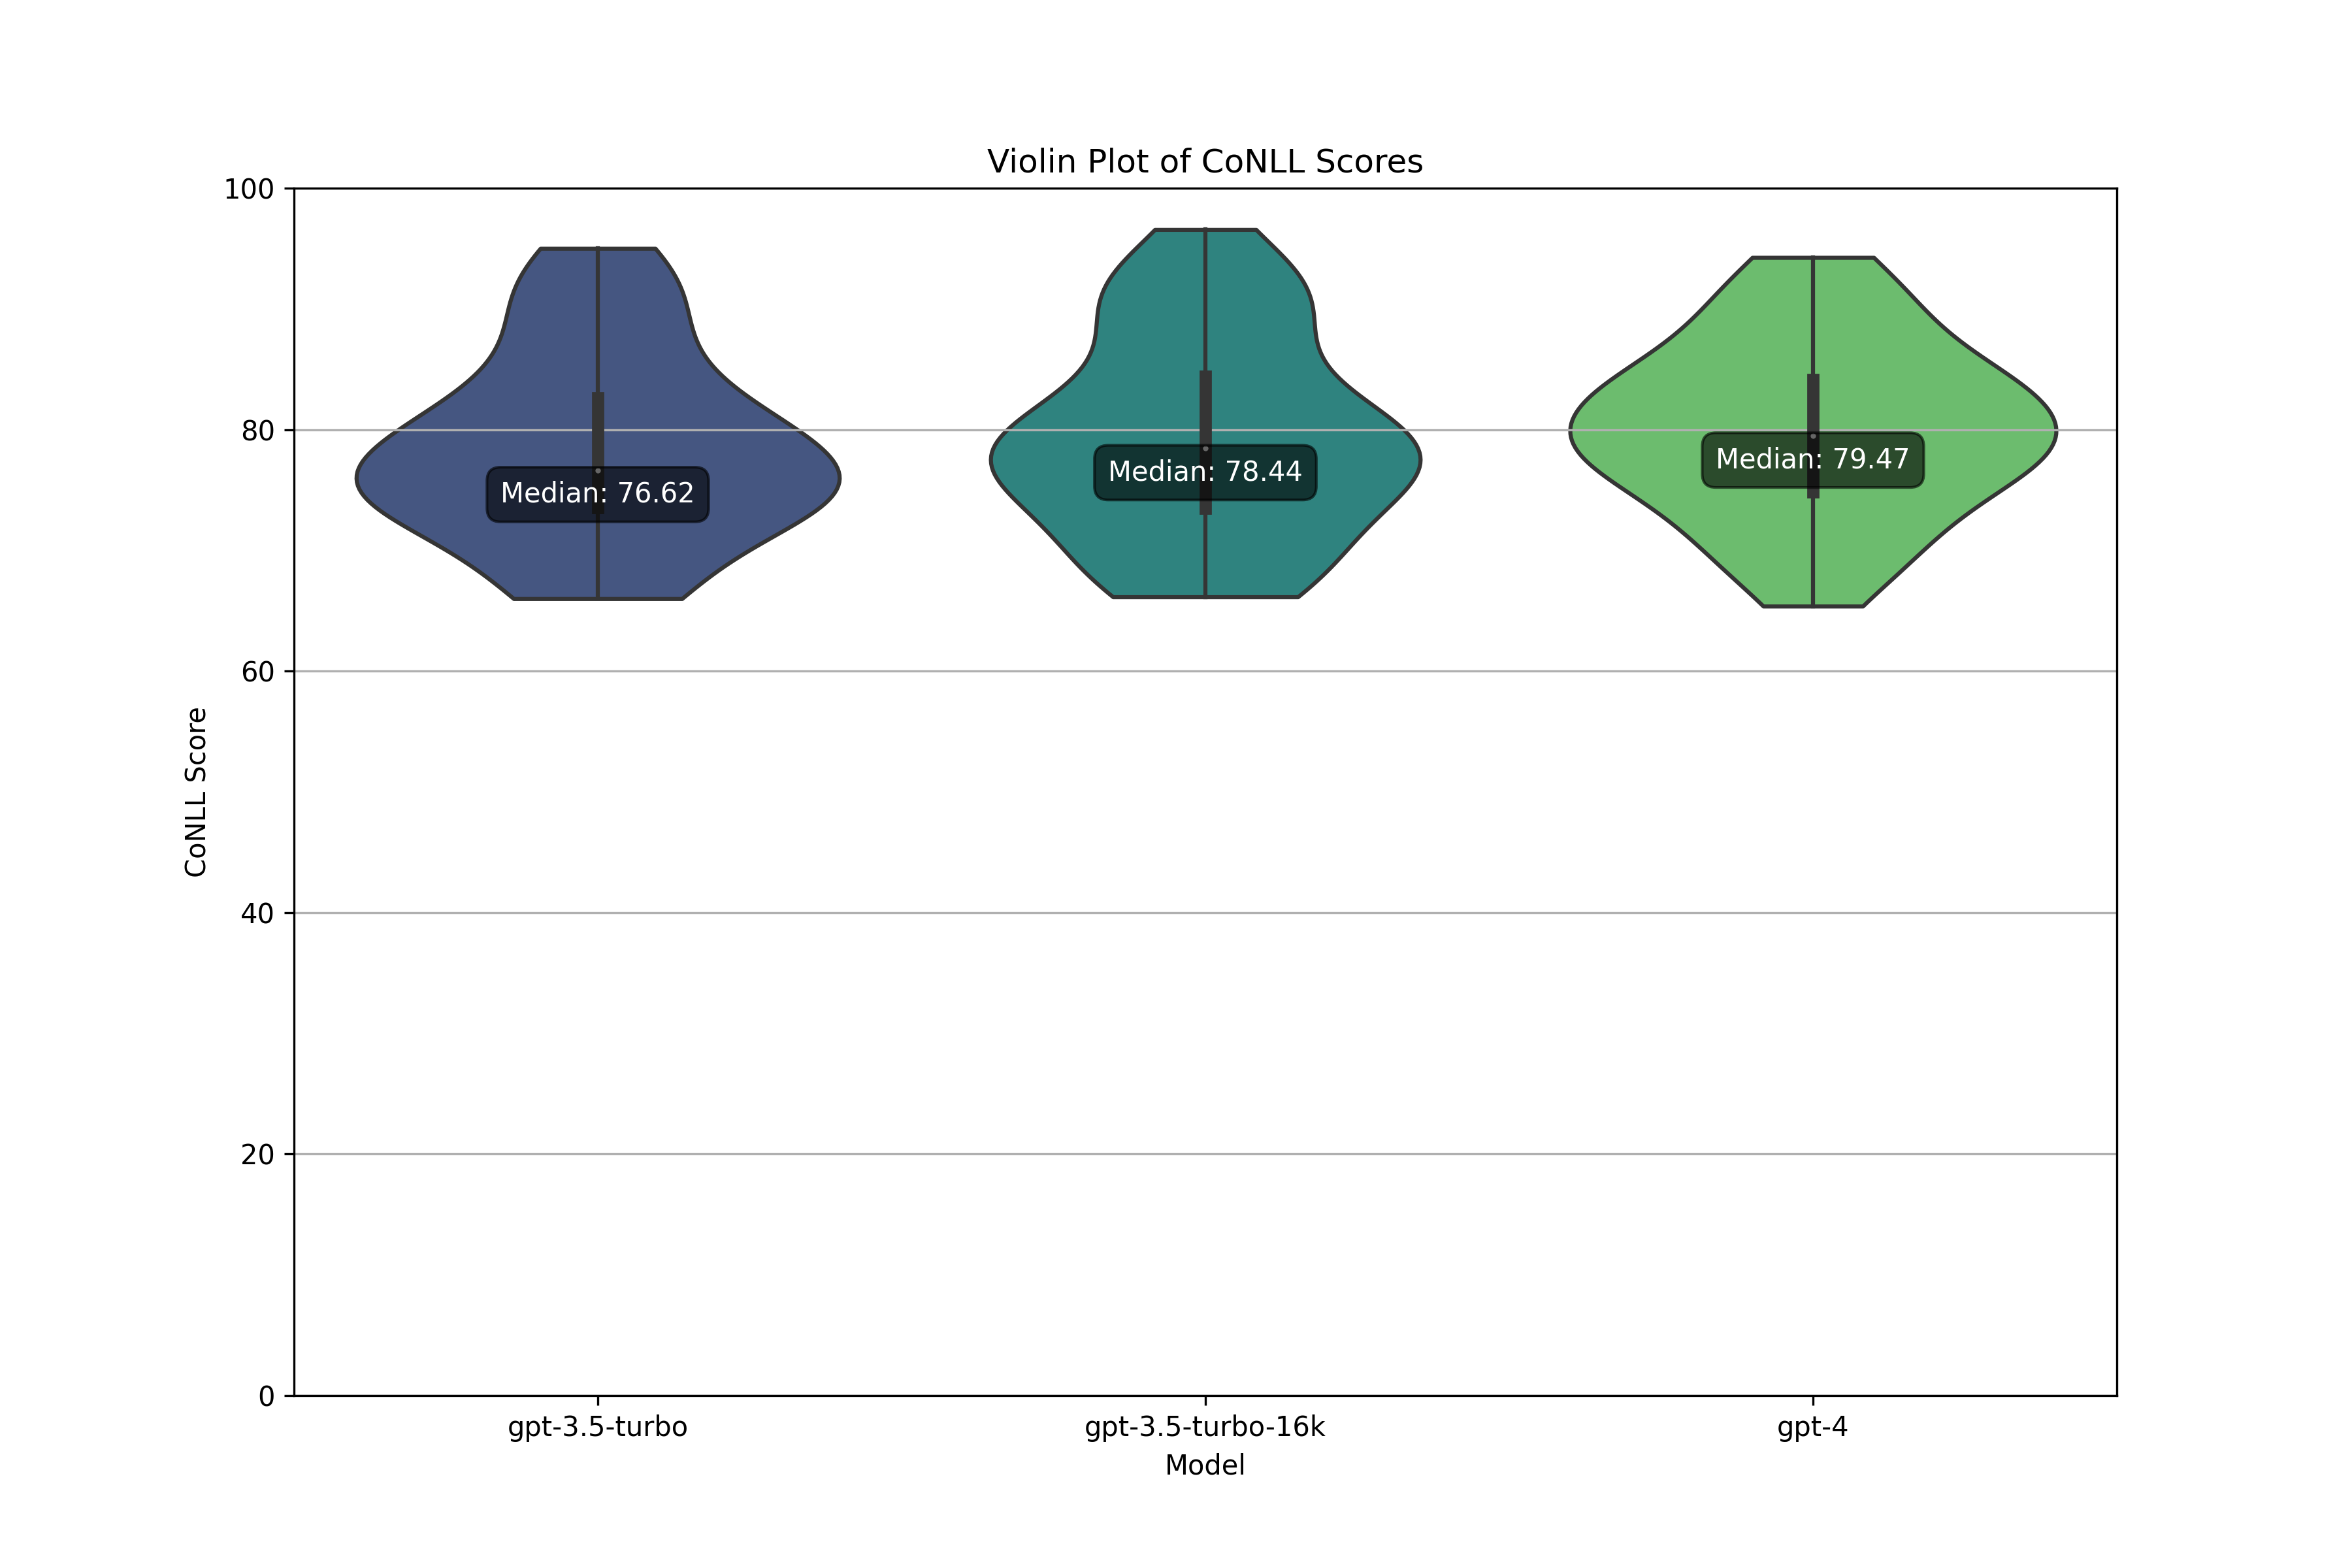
\includegraphics[width=14cm]{images/conll-score.png}
  \end{tabular}
  \caption[Distribution of CoNLL Score]{Violin Plot of CoNLL Score of all three different models}\label{fig:violin-conll}
\end{figure}

\subsection{Estimation of CoNLL Score}
Our deductions present that the computation of the CoNLL score is contingent upon four primary factors: 
    \begin{enumerate}
        \item Model: The hierarchy is clear — GPT4 outshines GPT-3.5-16k, which in turn surpasses GPT-3.5. 
        \item Topic: Our experiments revealed that papers from specific disciplines performed better — Logic outpaced NLP, which was further ahead of Astronomy, with Mathematics trailing them all. The underlying reason for this is perhaps the training data. Due to the open nature of OpenAI, it is impossible to verify this claim. Moreover, the inherent nature of Language Models struggling with Mathematics is perhaps another reason GPT suffered in Mathematics papers.
        \item Ambiguity pertains to the total number of discrete identifiers in the given paper. It goes without saying that the lower the number of identifiers, the better a model typically performs, as there are fewer distinctions to make. For example, in the formula $x = \frac{-b \pm \sqrt{b^2 - 4ac}}{2a}$ there are 4 identifiers, $x$, $a$, $b$, and $c$.
        \item Obscurity: This is estimated using the interquartile range of a given identifier's occurrences, focusing solely on the middle quartile and disregarding the outliers. From the same example of the quadratic equation of $x = \frac{-b \pm \sqrt{b^2 - 4ac}}{2a}$, $x$ and $c$ are repeated once but $a$ and $b$ are repeated twice. The rationale for focusing on the middle 40th percentile range is twofold. First, due to their limited occurrences, identifiers that appear infrequently (in the bottom 30th percentile) are generally easier for GPT to disambiguate. Second, persistent identifiers (in the top 30th percentile) may challenge annotation. However, our annotation approach results in a cascading effect that minimises its impact on the CoNLL score. Therefore, the identifiers falling within the middle 40th percentile truly contribute to the level of Obscurity. This subset is the primary focus when estimating the CoNLL score for annotation accuracy.
    \end{enumerate}

These four variables help devise a robust mathematical formula to estimate the CoNLL score, with the computation process detailed in Figure \ref{fig:conll-estimation}. Despite the limited sample size, preliminary results in Table \ref{tab:mse-r2} demonstrate the potential of this predictive model.

\clearpage

\begin{figure}[htpb]
  \begin{equation}
      \text{estimated\_conll\_score} \simeq \frac{-2}{5} \times \text{total\_concepts} + \frac{-1}{5} \times \text{occur\_iqr} + \text{intercept}
  \end{equation}
  \caption[CoNLL Estimation]{Estimate the CoNLL Score for NLP Papers}
  \label{fig:conll-estimation}
\end{figure}

In the equation above, the variables are defined as follows:
\begin{itemize}
  \item \textbf{estimated\_conll\_score} is the estimated CoNLL score.
  \item \textbf{total\_concepts} is the total number of concepts in the paper (Ambiguity).
  \item \textbf{occur\_iqr} represents (Obscurity).
  \item \textbf{intercept} is the y-intercept which depends on the model. gpt-3.5 = 93, gpt-3.5-16k = 95, gpt-4 = 97.
\end{itemize}

Figure \ref{fig:esimated-conll} shows the visualisation of our novel formula on a 3D plane.

\begin{figure}[htpb]
  \centering
  \subfloat[Angled View]{
    \begin{tabular}{c}
  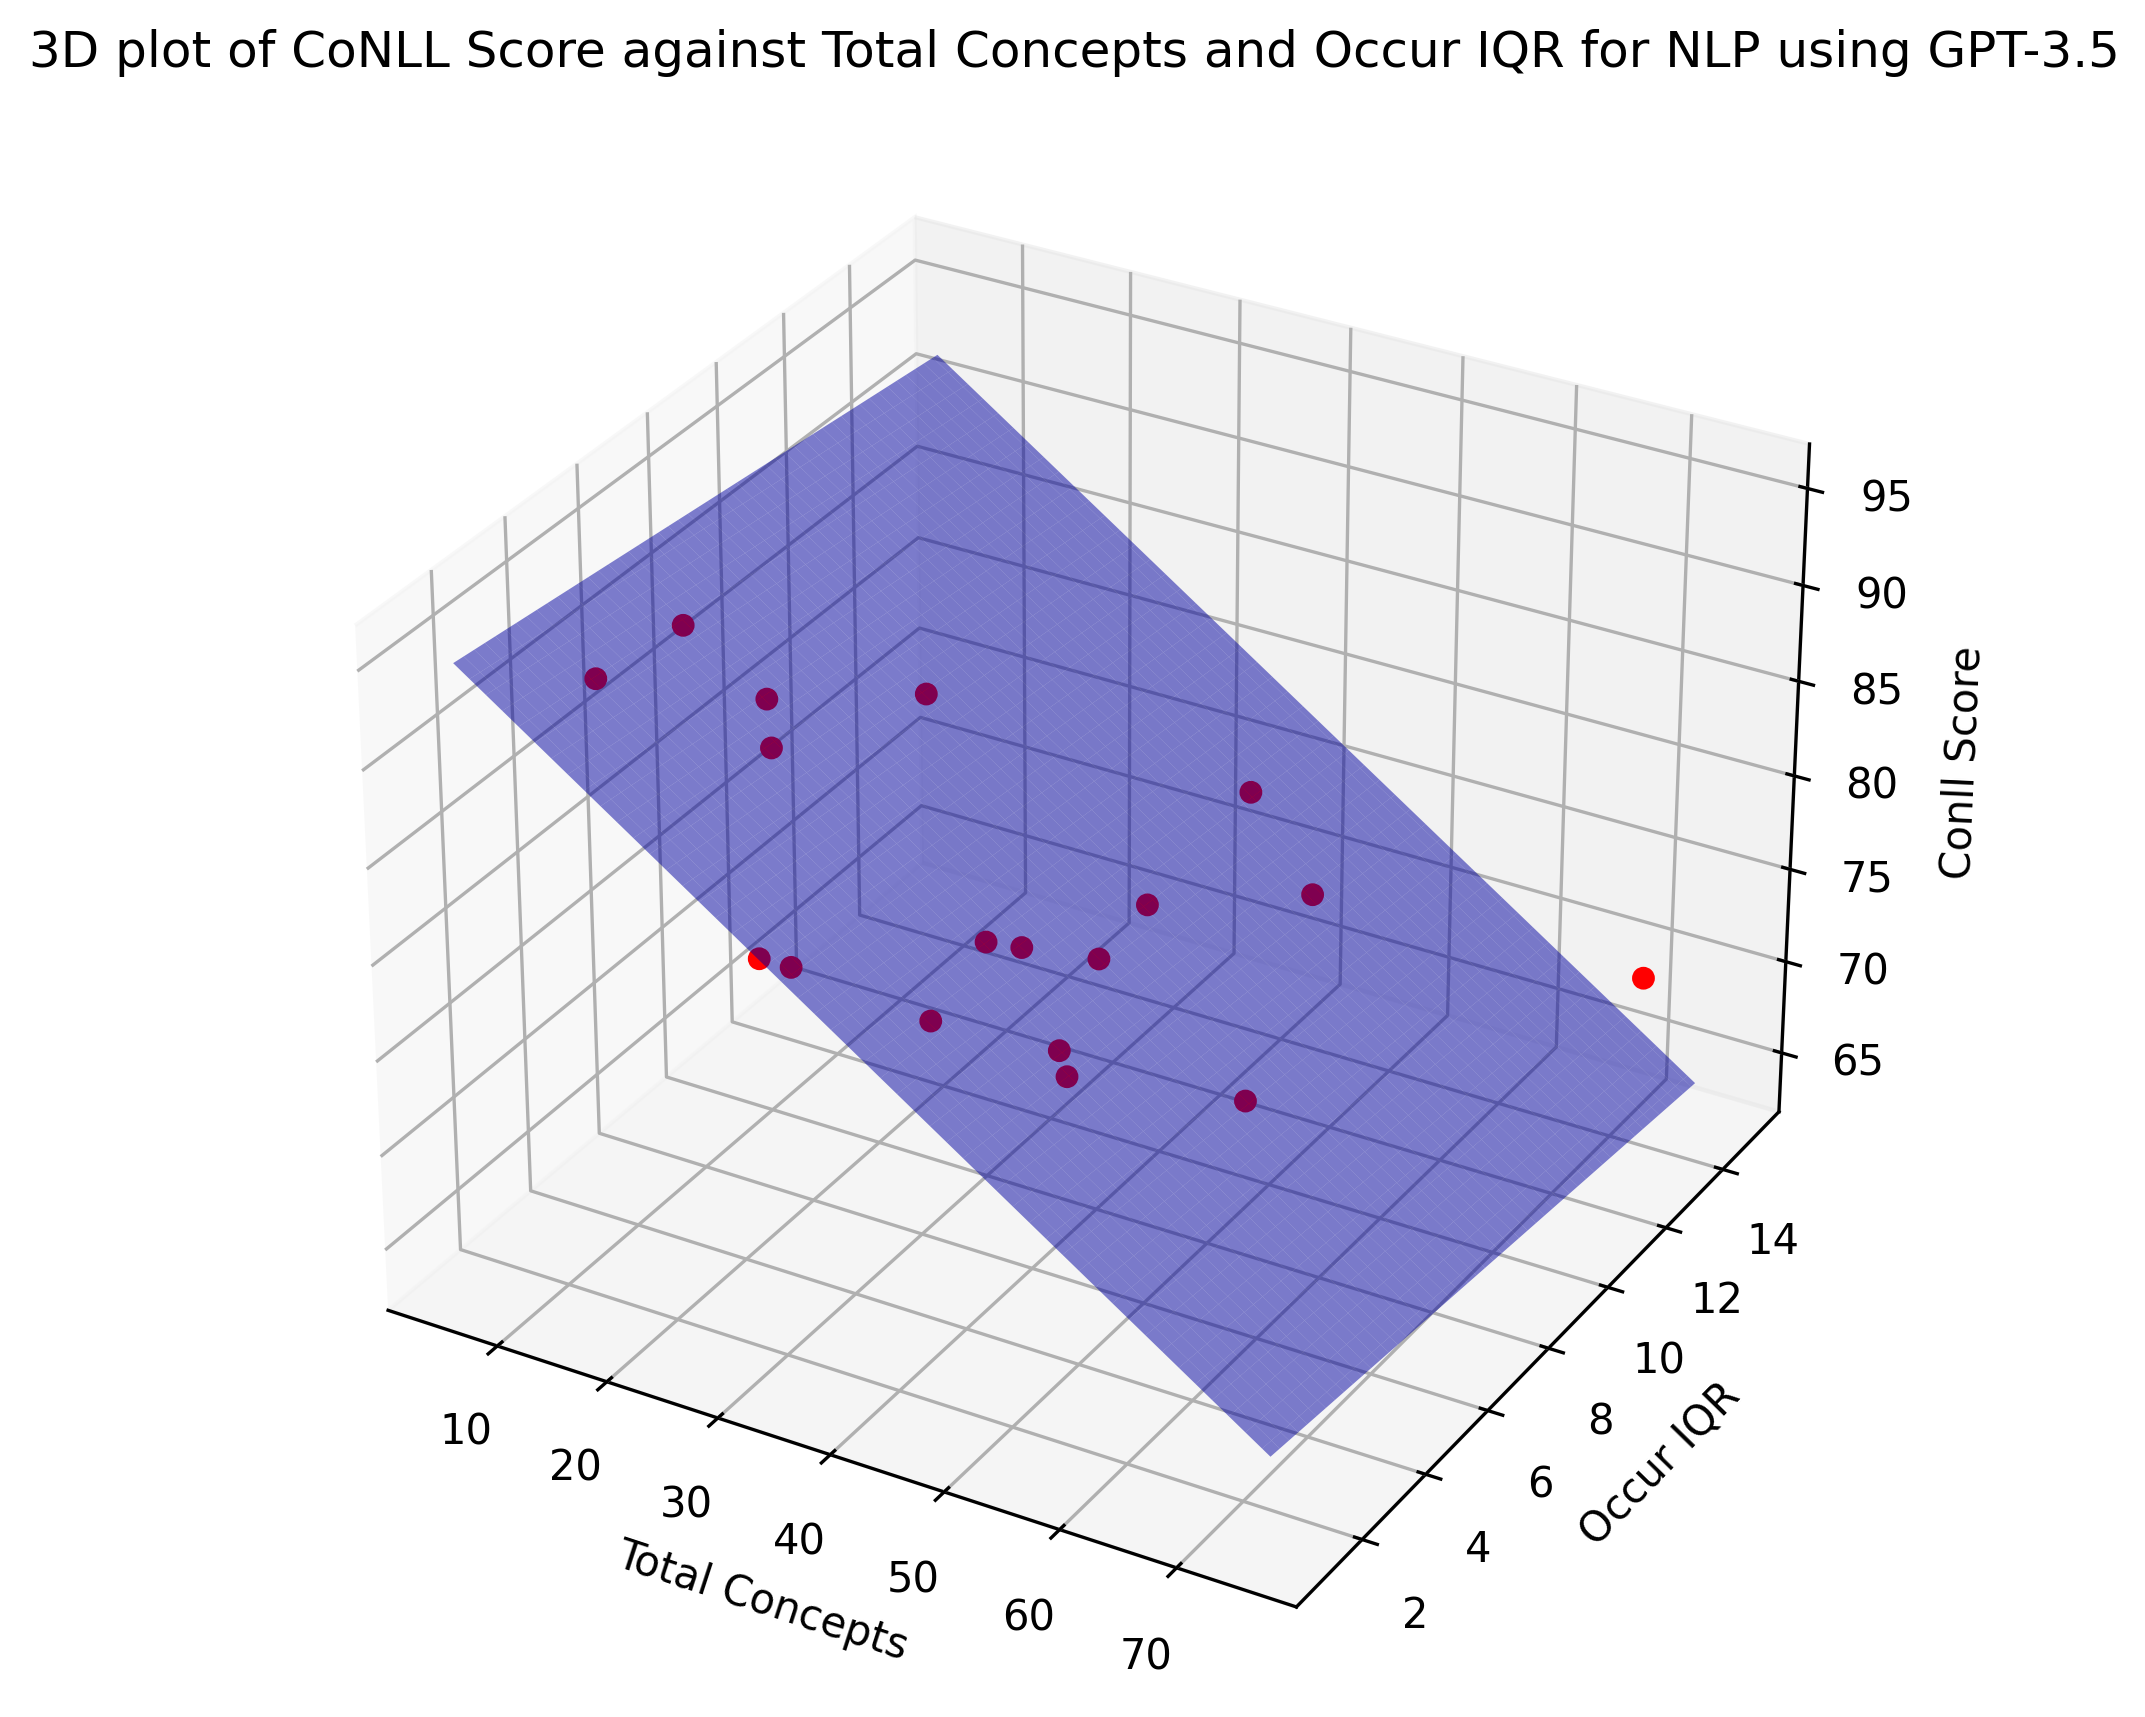
\includegraphics[width=11cm]{images/estimated-conll.png}
  \end{tabular}
  }
  \quad 
  \subfloat[Side view]{
    \begin{tabular}{c}
  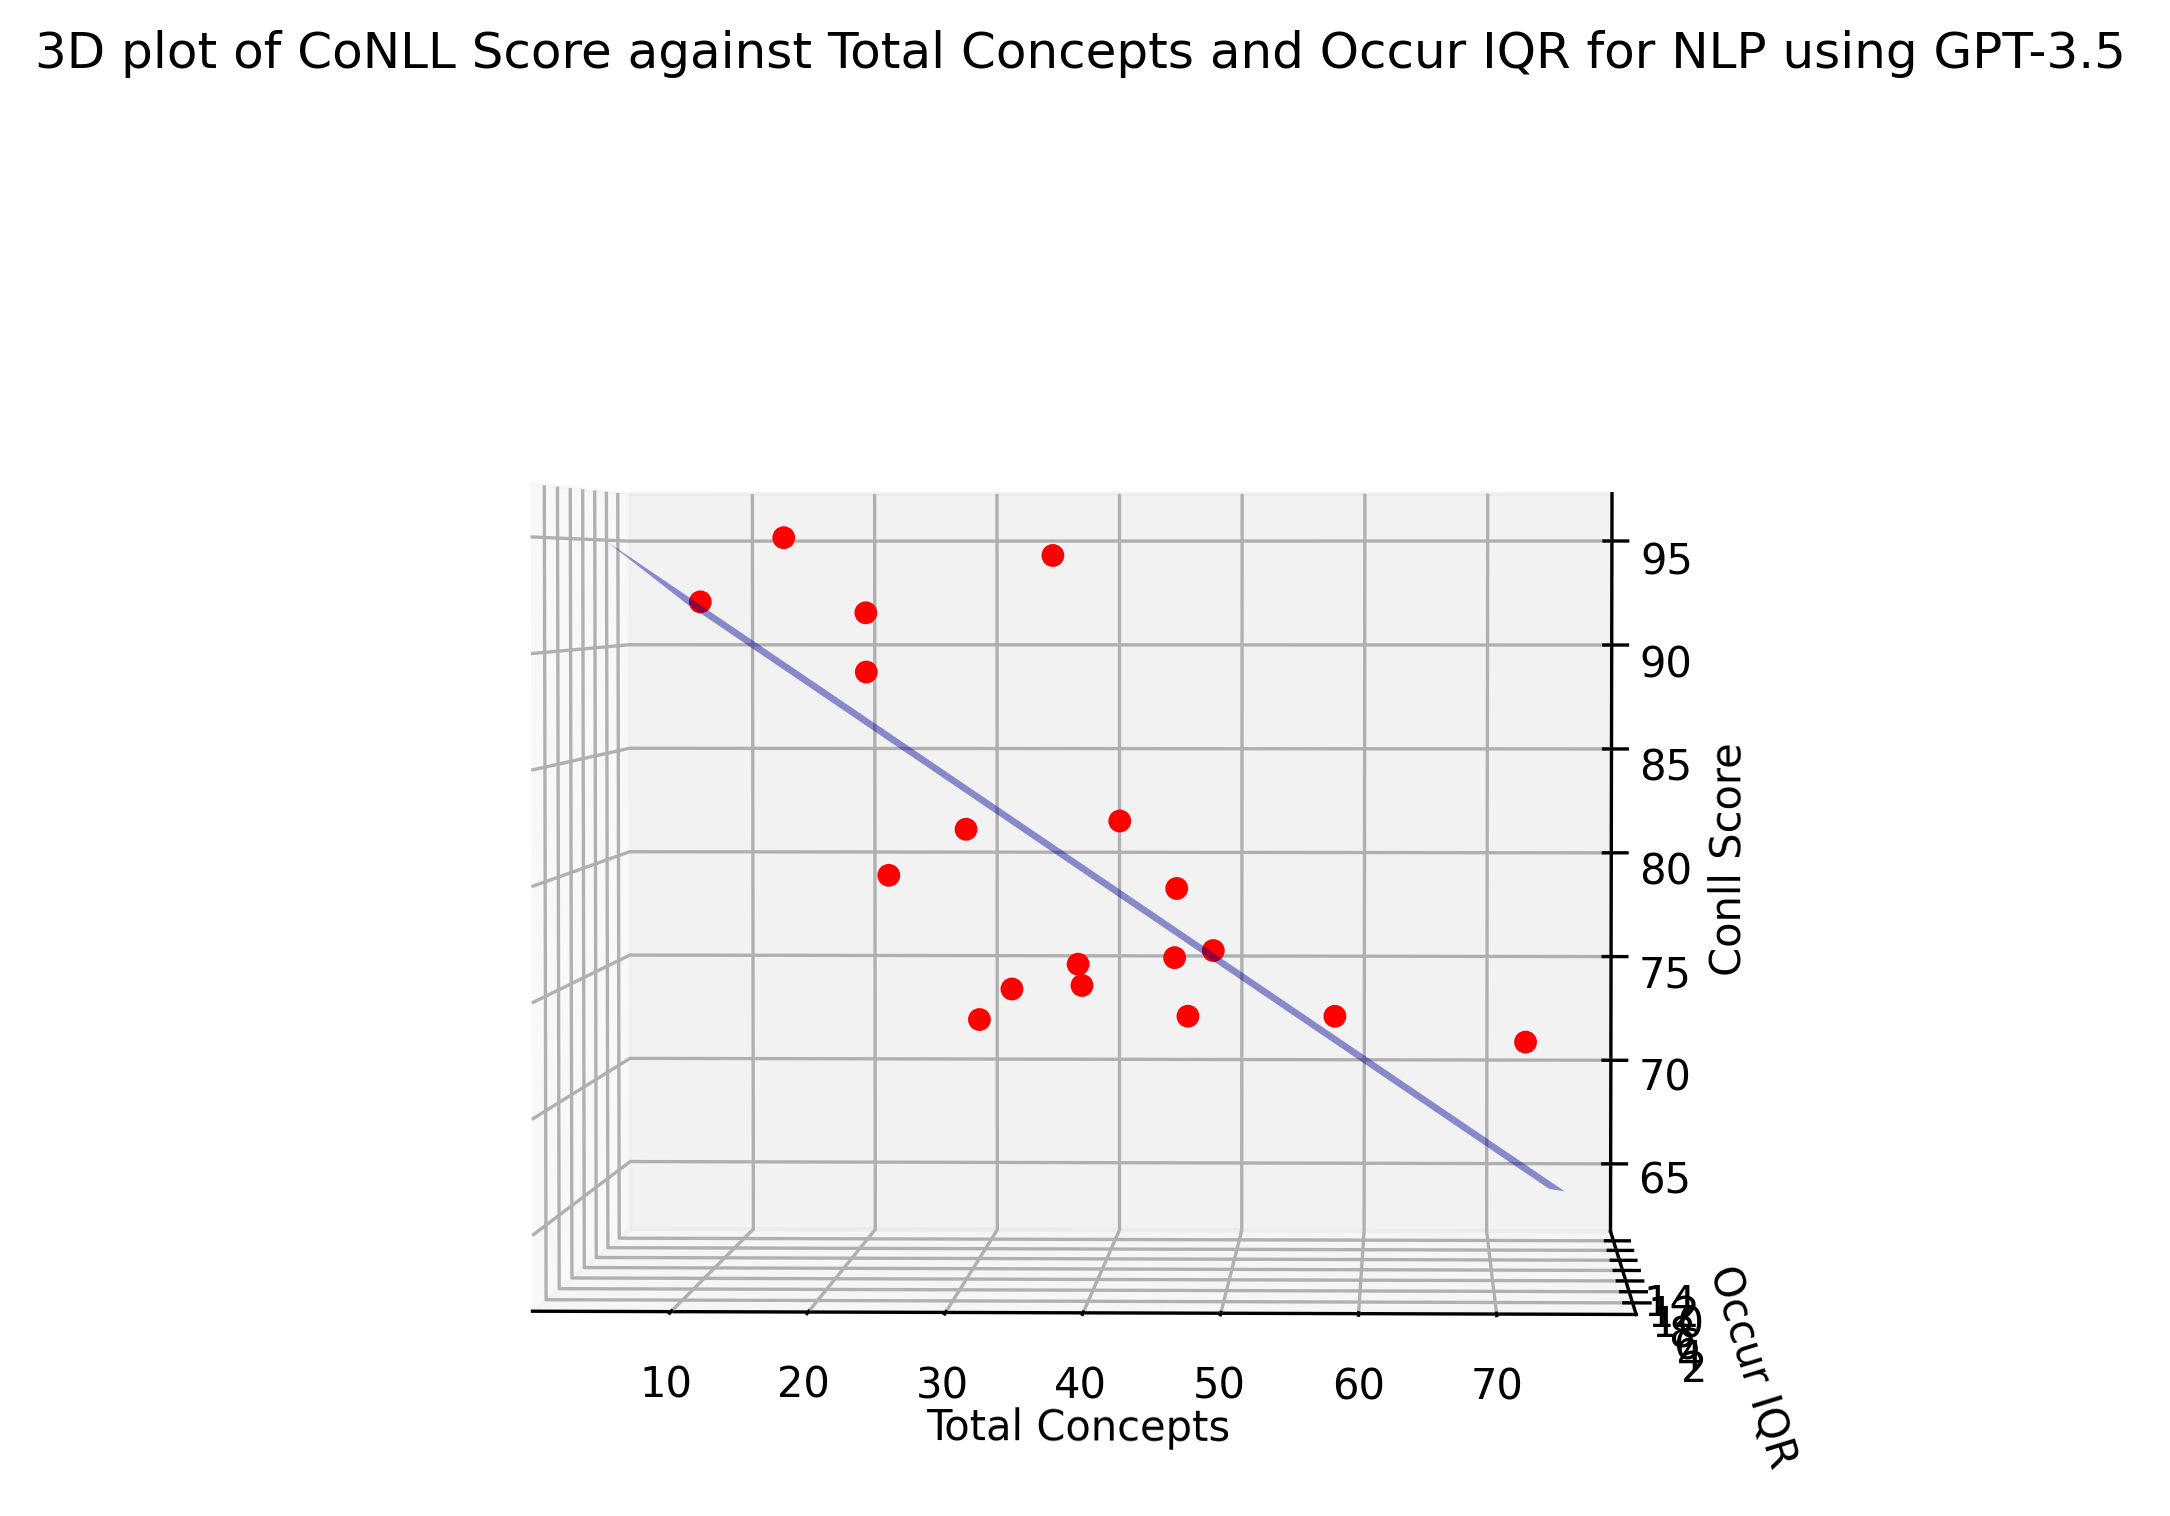
\includegraphics[width=11cm]{images/estimated-conll-2.png}
  \end{tabular}
  }
  \caption[CoNLL Score Estimation]{3D Visualisation of the CoNLL Score Estimation Formula}\label{fig:esimated-conll}
\end{figure}

Table \ref{tab:mse-r2} shows the estimation formula's Mean Square Error and R2 Score. Since there were only 18 papers in hand for NLP, getting better results was difficult.

\begin{table}[h]
    \centering
    \begin{tabular}{lrr}
        \hline
        Model & Mean Square Error & R2 Score \\
        \hline
        GPT-3.5-turbo & 35.636 & 0.136 \\
        GPT-3.5-16k-turbo & 25.936 & 0.371 \\
        GPT-4 & 26.386 & 0.360 \\
        \hline
    \end{tabular}
    \caption{Mean Square Error and R2 Score of the Estimation Formula}
    \label{tab:mse-r2}
\end{table}

\subsection{Coverage of Annotation}

The coverage of annotation refers to the proportion of the paper that the LLMs successfully annotated. Consistent with the CoNLL results, GPT-4 again made a mark by consistently outperforming the other two GPT models. GPT-3.5-16k, in contrast, had lesser coverage than GPT-3.5 due to the former's instability and propensity for repetition death. Figure \ref{fig:violin-coverage} provides a visual representation of the coverage exhibited by all three models.

\begin{figure}[htpb]
  \centering
  \begin{tabular}{c}
  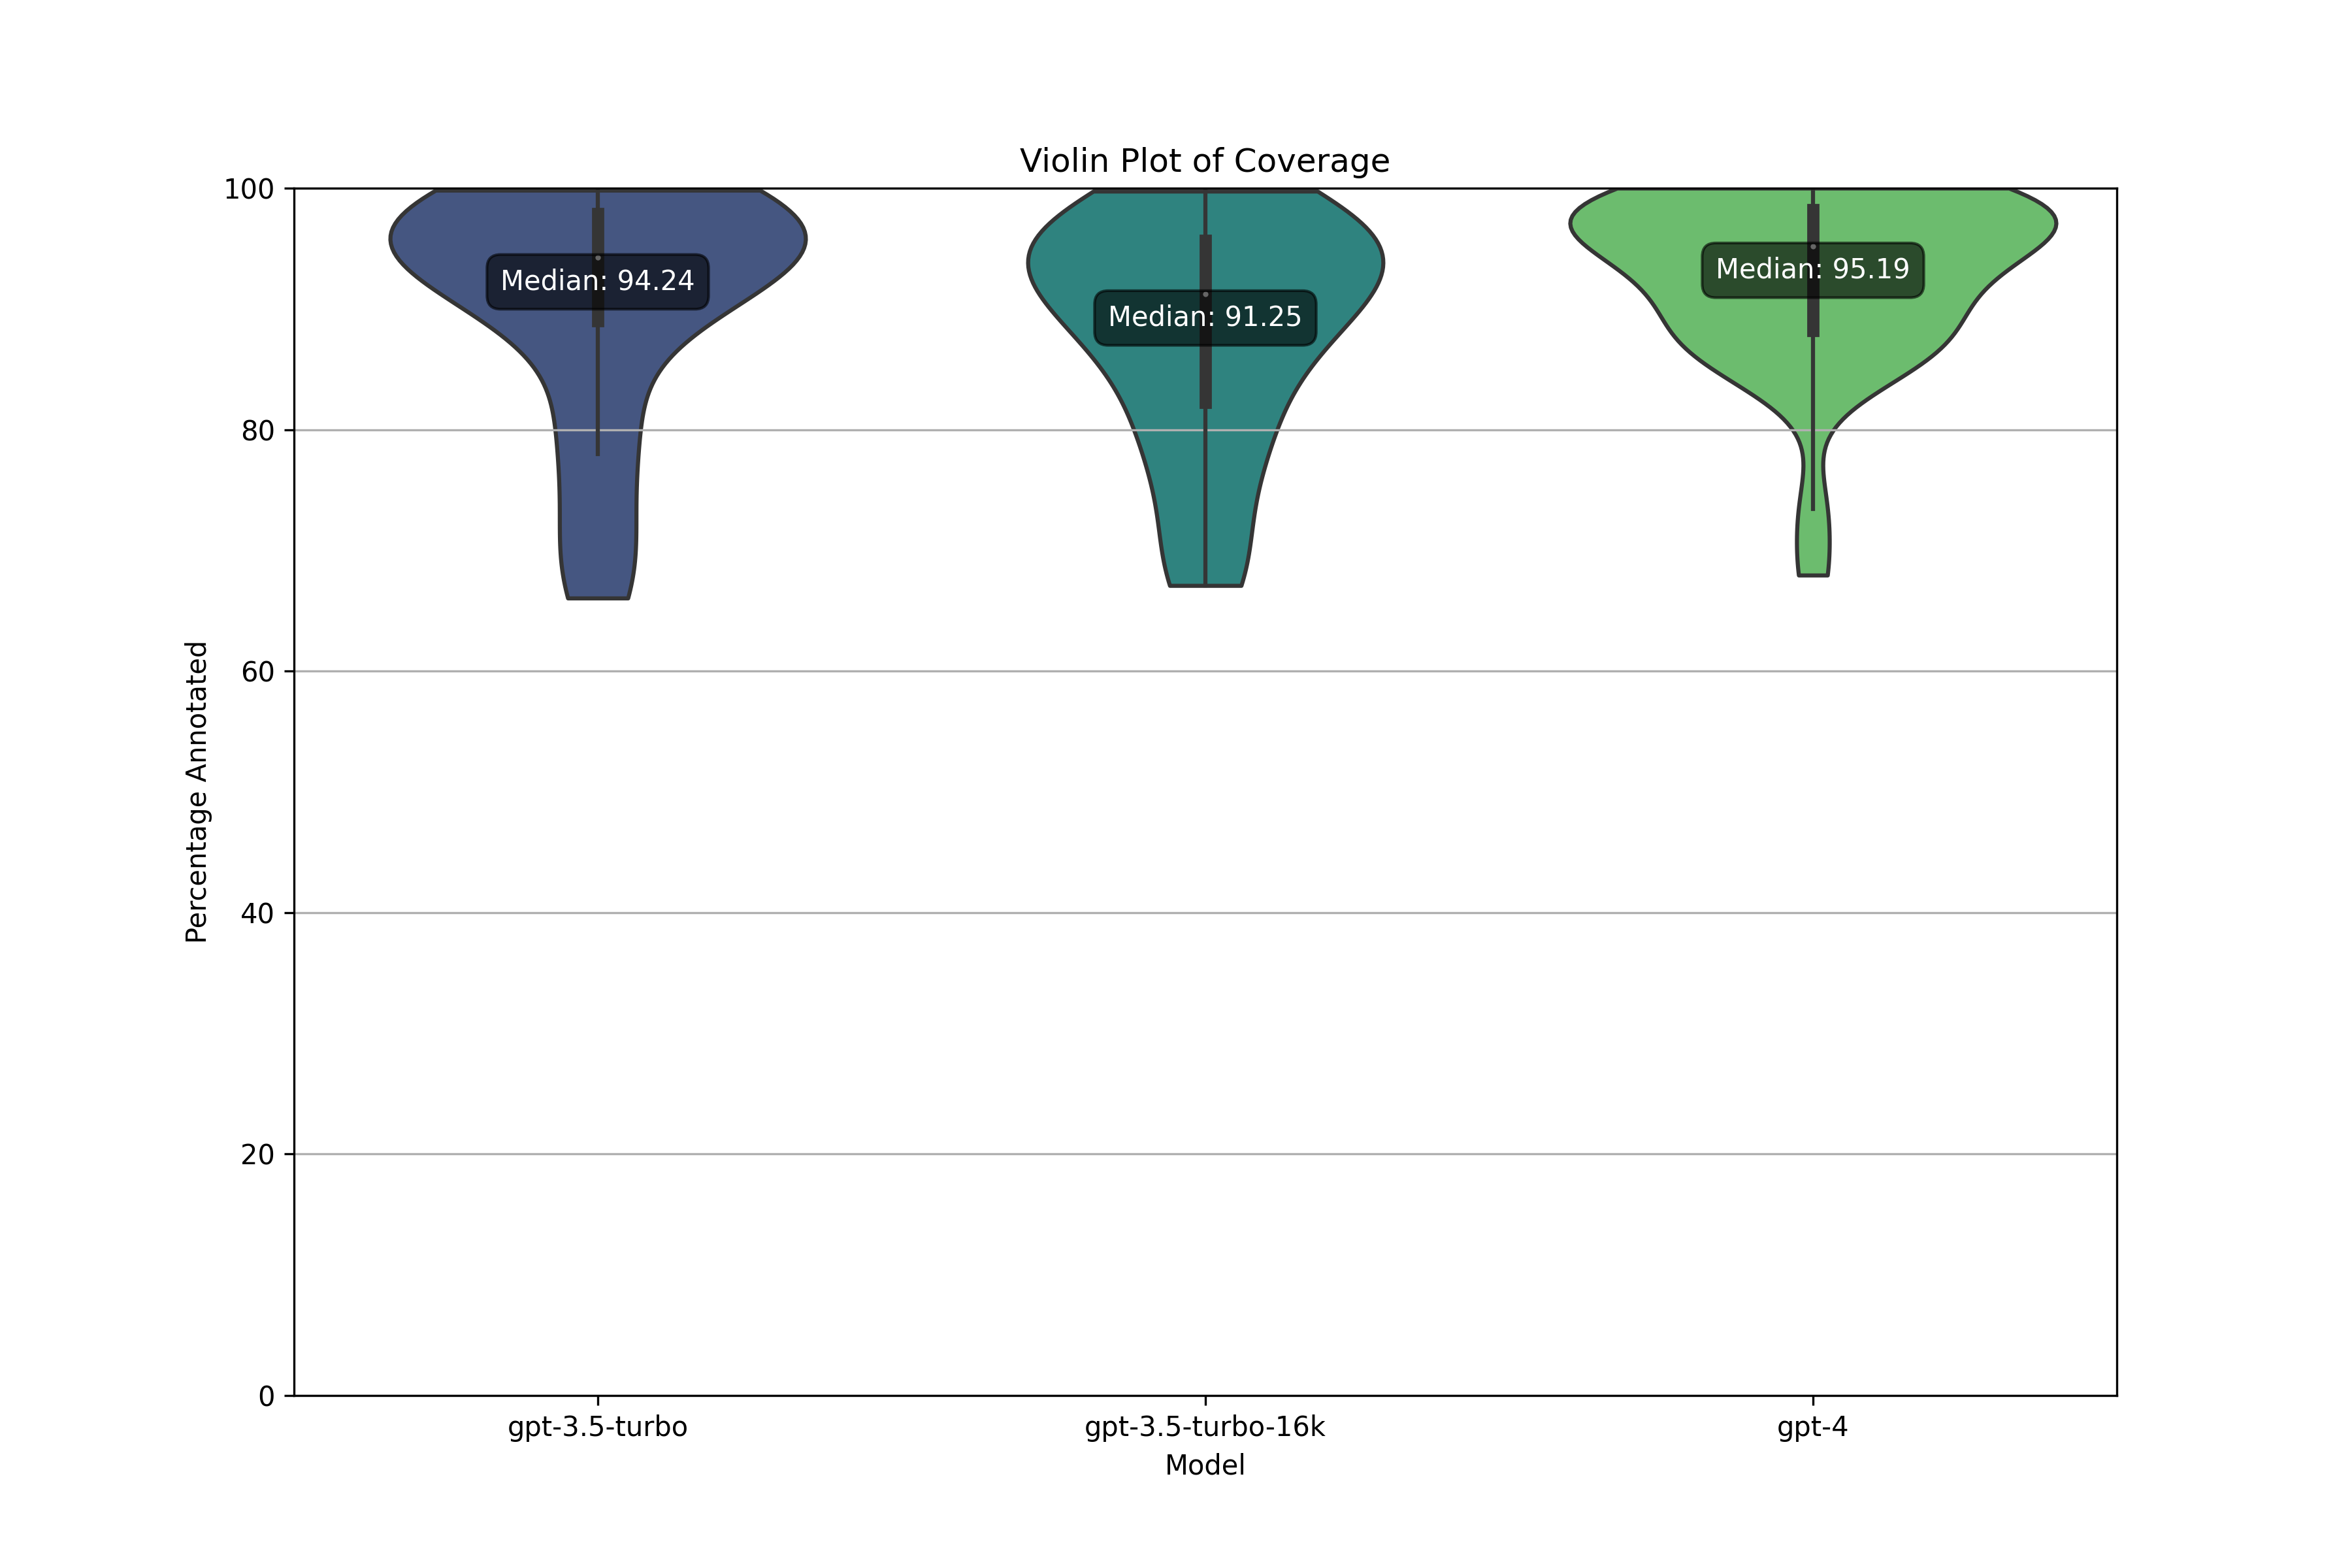
\includegraphics[width=14cm]{images/coverage.png}
  \end{tabular}
  \caption[Distribution of Coverage]{Violin Plot of the Coverage of Annotations of all three different models}\label{fig:violin-coverage}
\end{figure}
 
\subsection{Semantic Accuracy}

Semantic accuracy provides a measure of the correctness of the annotations. We weighted it against the coverage to represent the total. Because of the extensive difficulty of manually reviewing semantic accuracy, we evaluated five carefully picked papers representing various low/high CoNLL scores and lengths. As detailed in Figure \ref{fig:violin-semantic}, GPT-4 consistently outperformed all the other models by a significant margin. There were a few papers where GPT-4 achieved an astonishing 100\% semantic accuracy, but weighing it with coverage brings it down to 98\%. GPT-4's worst performance is almost as good as the best performances of other models, marking it as superior. This comes as no surprise as GPT-4 is one of the largest LLMs as of writing this thesis.

\begin{figure}[htpb]
  \centering
  \begin{tabular}{c}
  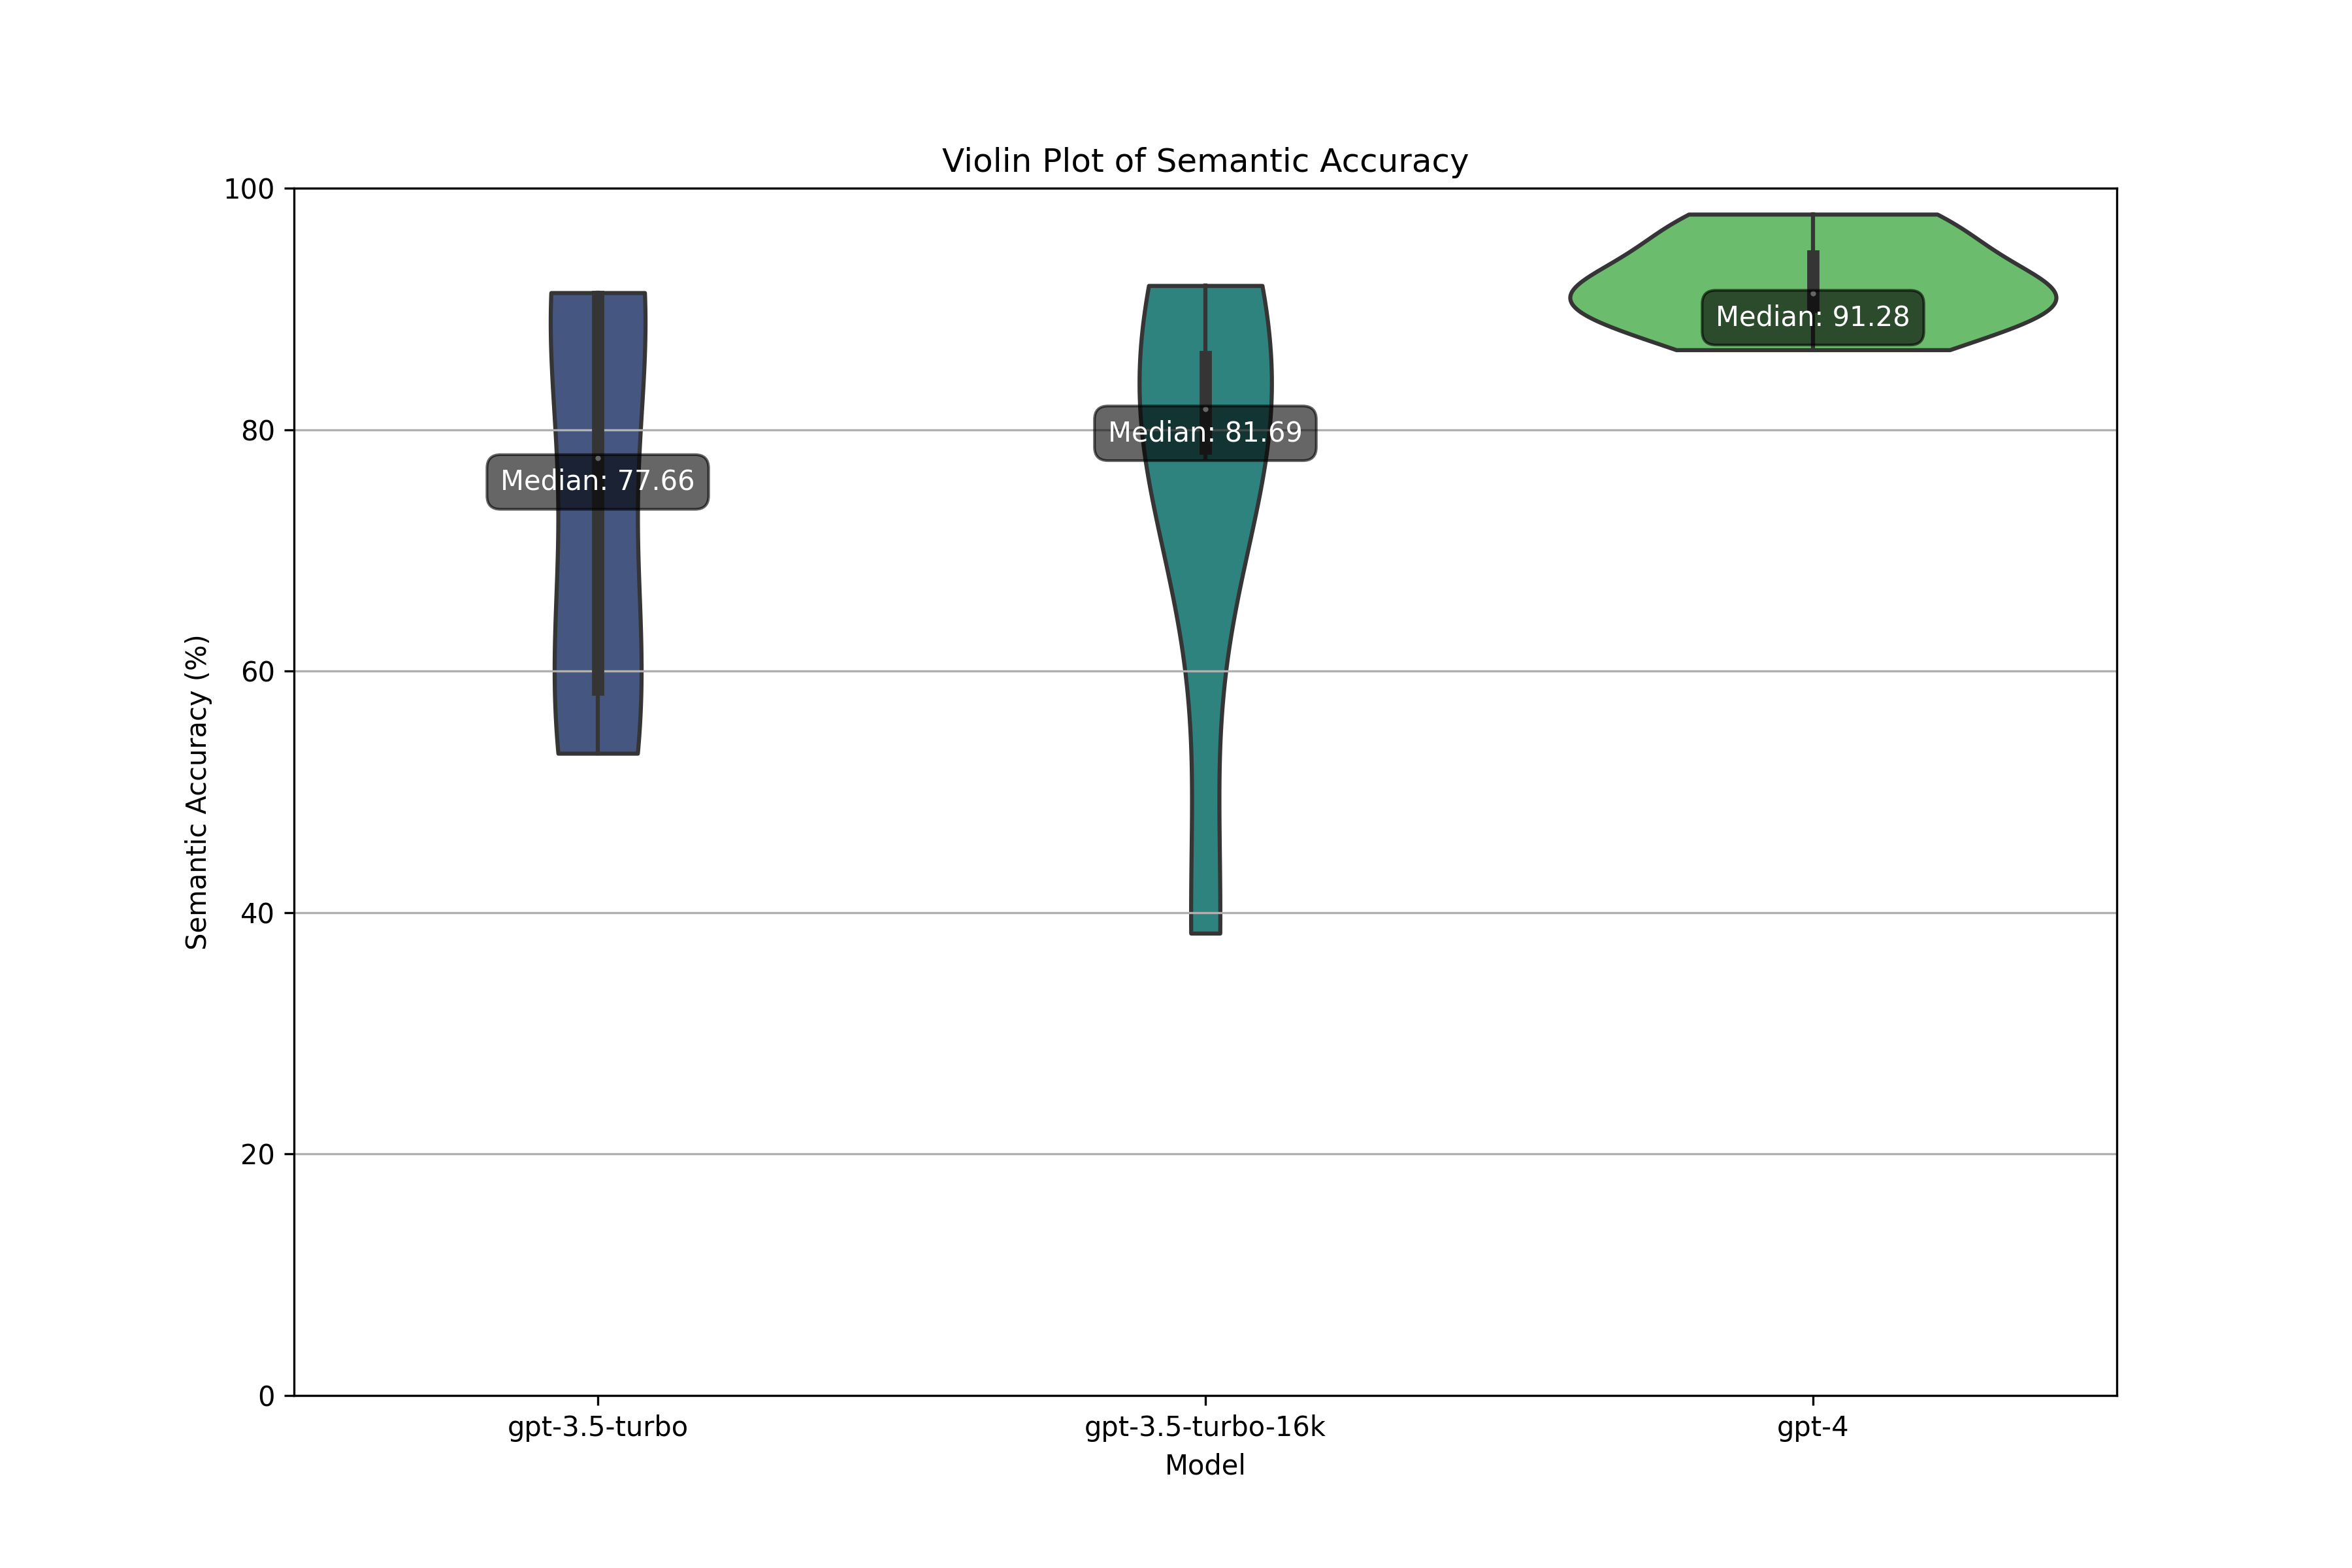
\includegraphics[width=14cm]{images/semantic-accuracy.png}
  \end{tabular}
  \caption[Semantic Accuracy]{Violin Plot of the Weighted Semantic Accuracy of all GPT Models}\label{fig:violin-semantic}
\end{figure}

\subsection{Variance of Data}

To account for these models' stochastic nature and ensure our experiment's reproducibility and stability, we sampled one reference paper, ArXiV ID: 2107.10832 \citep{singleton2021logic}. We ran the experiment four times, evaluating the variance in the CoNLL scores. GPT-3.5 and GPT-4 proved monumentally stable, whereas GPT-3.5-16k, a newer model, still exhibited volatility issues. These outcomes are displayed in Figure \ref{fig:violin-variance}.

\begin{figure}[htpb]
  \centering
  \begin{tabular}{c}
  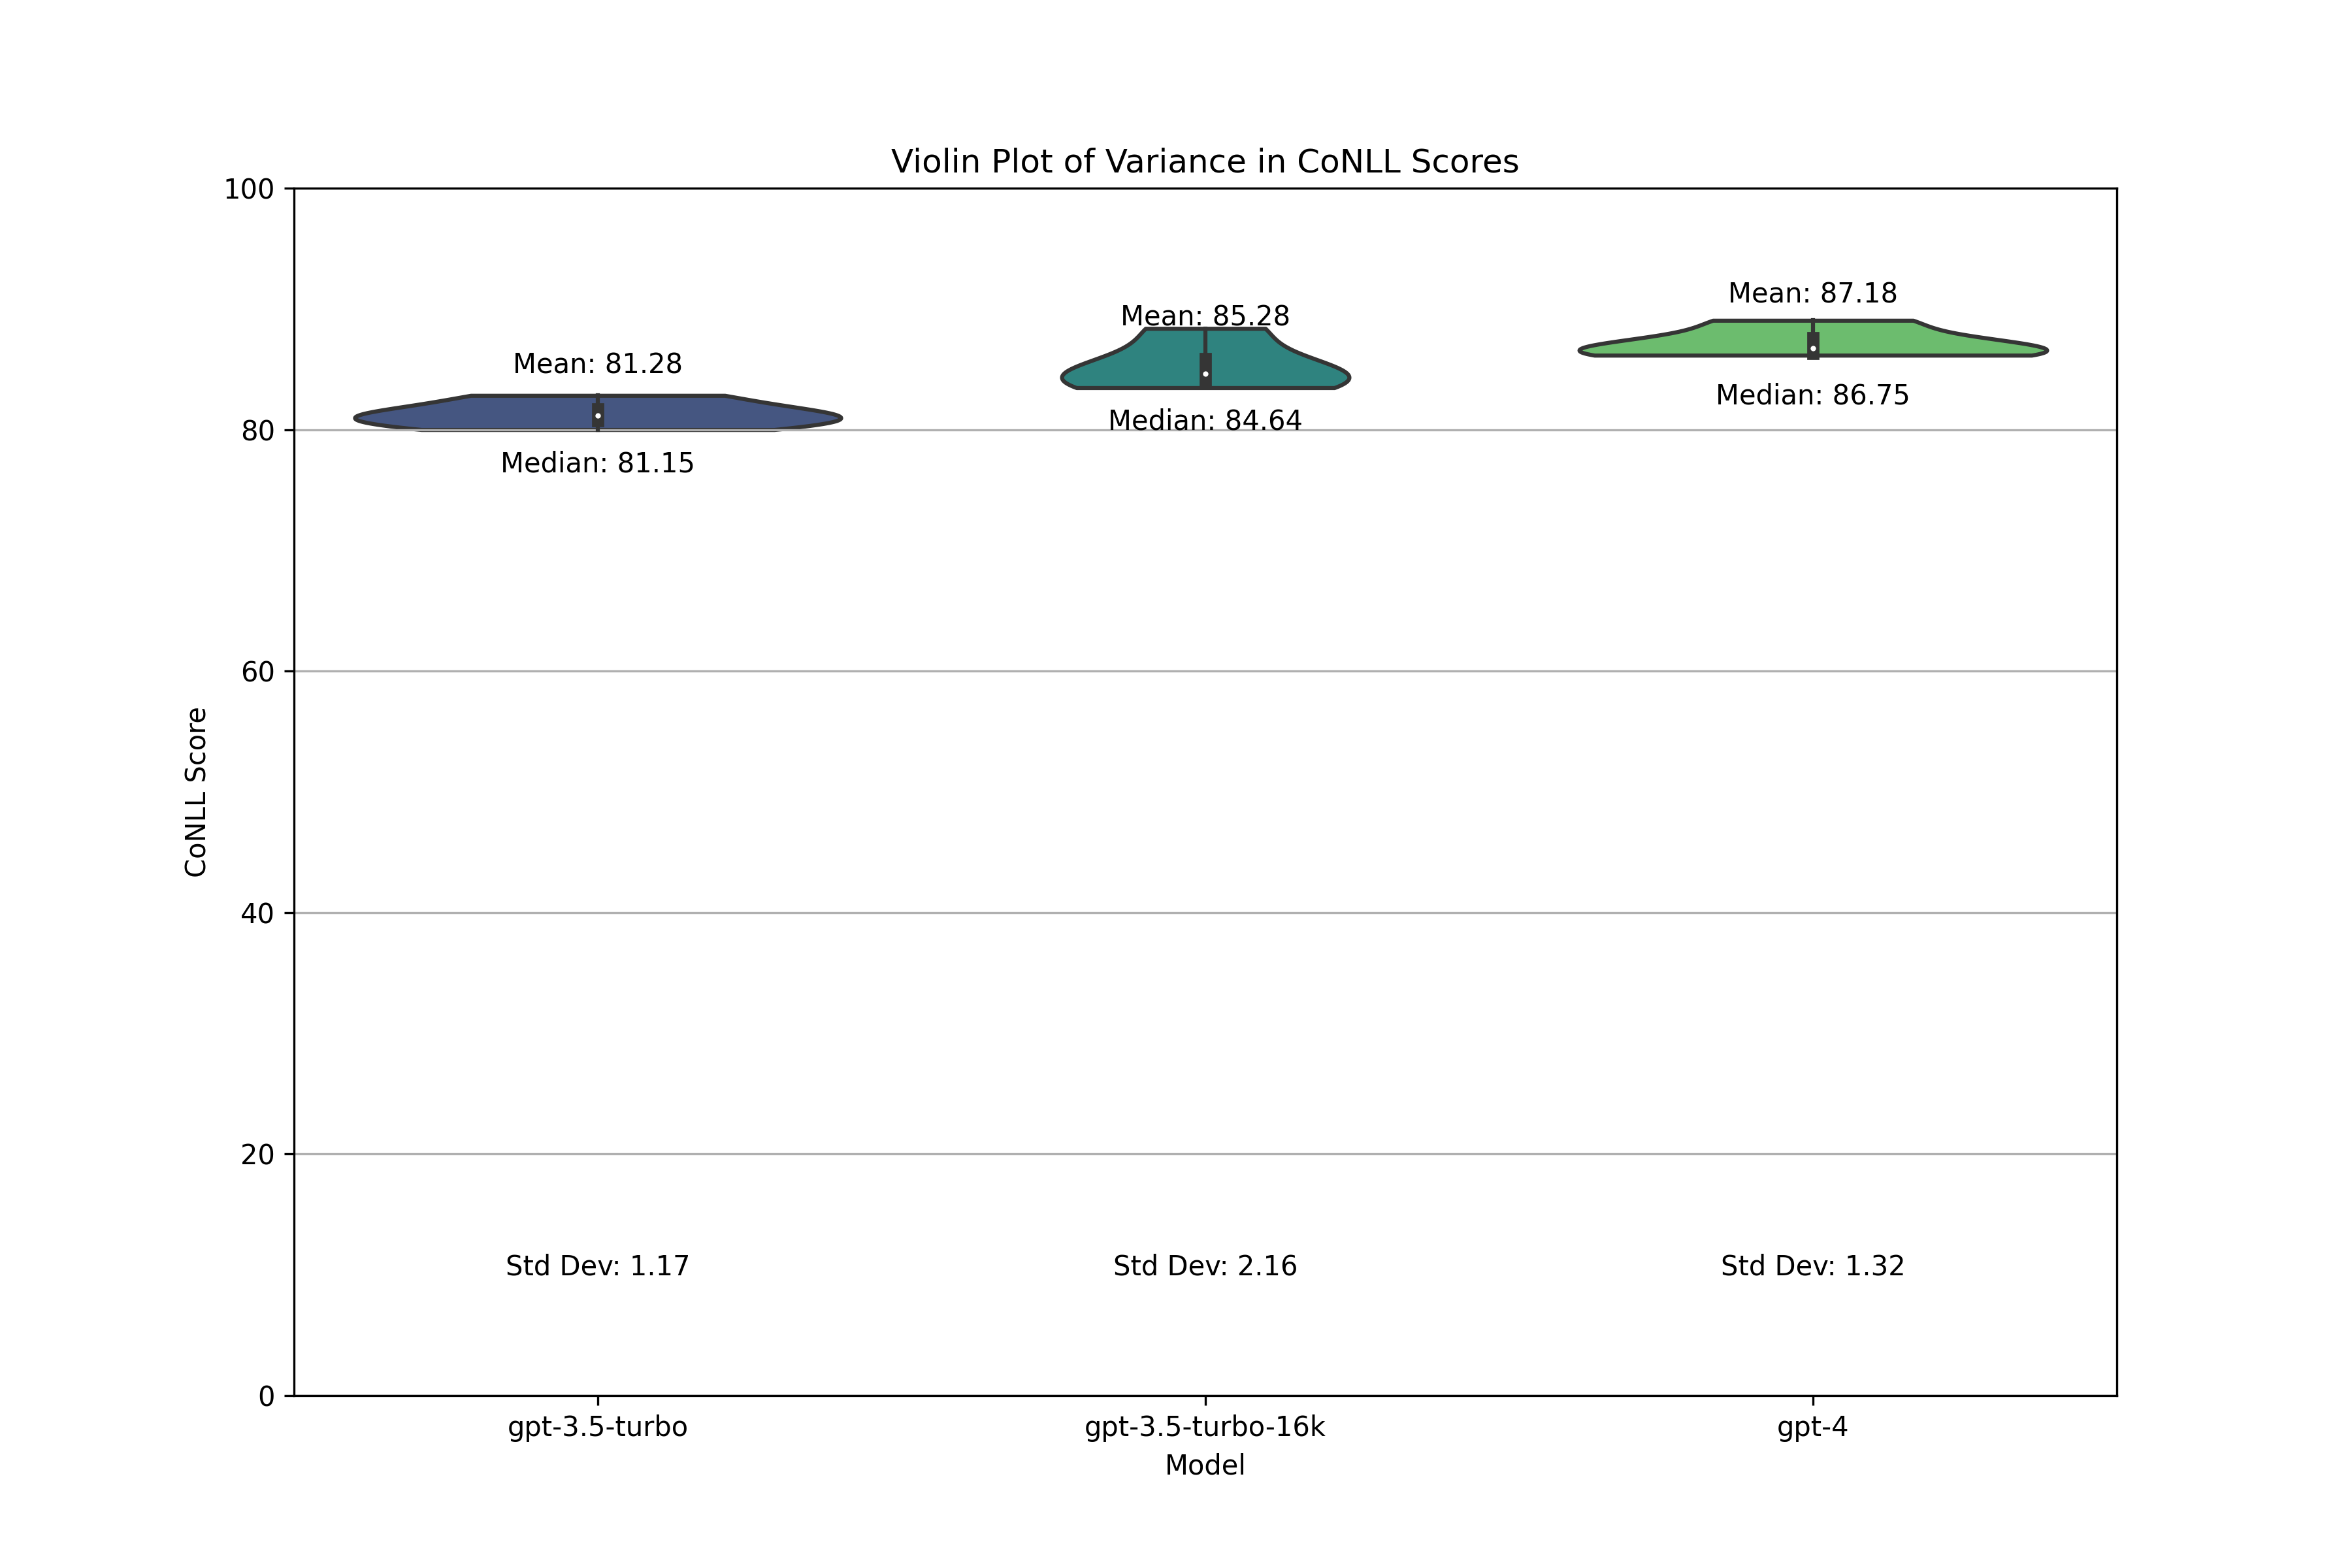
\includegraphics[width=14cm]{images/variance-conll.png}
  \end{tabular}
  \caption[The variance]{Violin Plot of the CoNLL scores for same paper four times}\label{fig:violin-variance}
\end{figure}

\subsection{Running Time and Costs}

The financial aspects of utilising GPT models are quantified through token usage. A comprehensive visualisation of the average costs and time durations for our experiments is provided in Figure \ref{fig:gpt-cost-anal}. It is crucial to note that the length of the paper influences both these metrics under consideration. To offer a more standardised comparison, we present the costs normalised per 1,000 annotations in Figure \ref{fig:gpt-relative-cost}.

Another pivotal dimension is the trade-off between cost and time efficiency. While the ideal scenario would be to minimise both, practical constraints often make this challenging. This relationship is further explored in Figure \ref{fig:gpt-time-v-cost}.

GPT-3.5 emerged as the most cost-effective and time-efficient option among the models evaluated. This efficiency is attributable to OpenAI's competitive token pricing and additional optimisations. Conversely, GPT-4 incurred the highest expenses due to its elevated token costs. GPT-3.5 and GPT-4 demonstrated remarkable stability, contributing to their lower time expenditures. On the other hand, GPT-3.5-16k exhibited instability, leading to increased time costs.

\begin{figure}[htpb]
  \centering
  \subfloat[Average Cost of Annotation]{
    \begin{tabular}{c}
  \hspace*{-.25cm}
  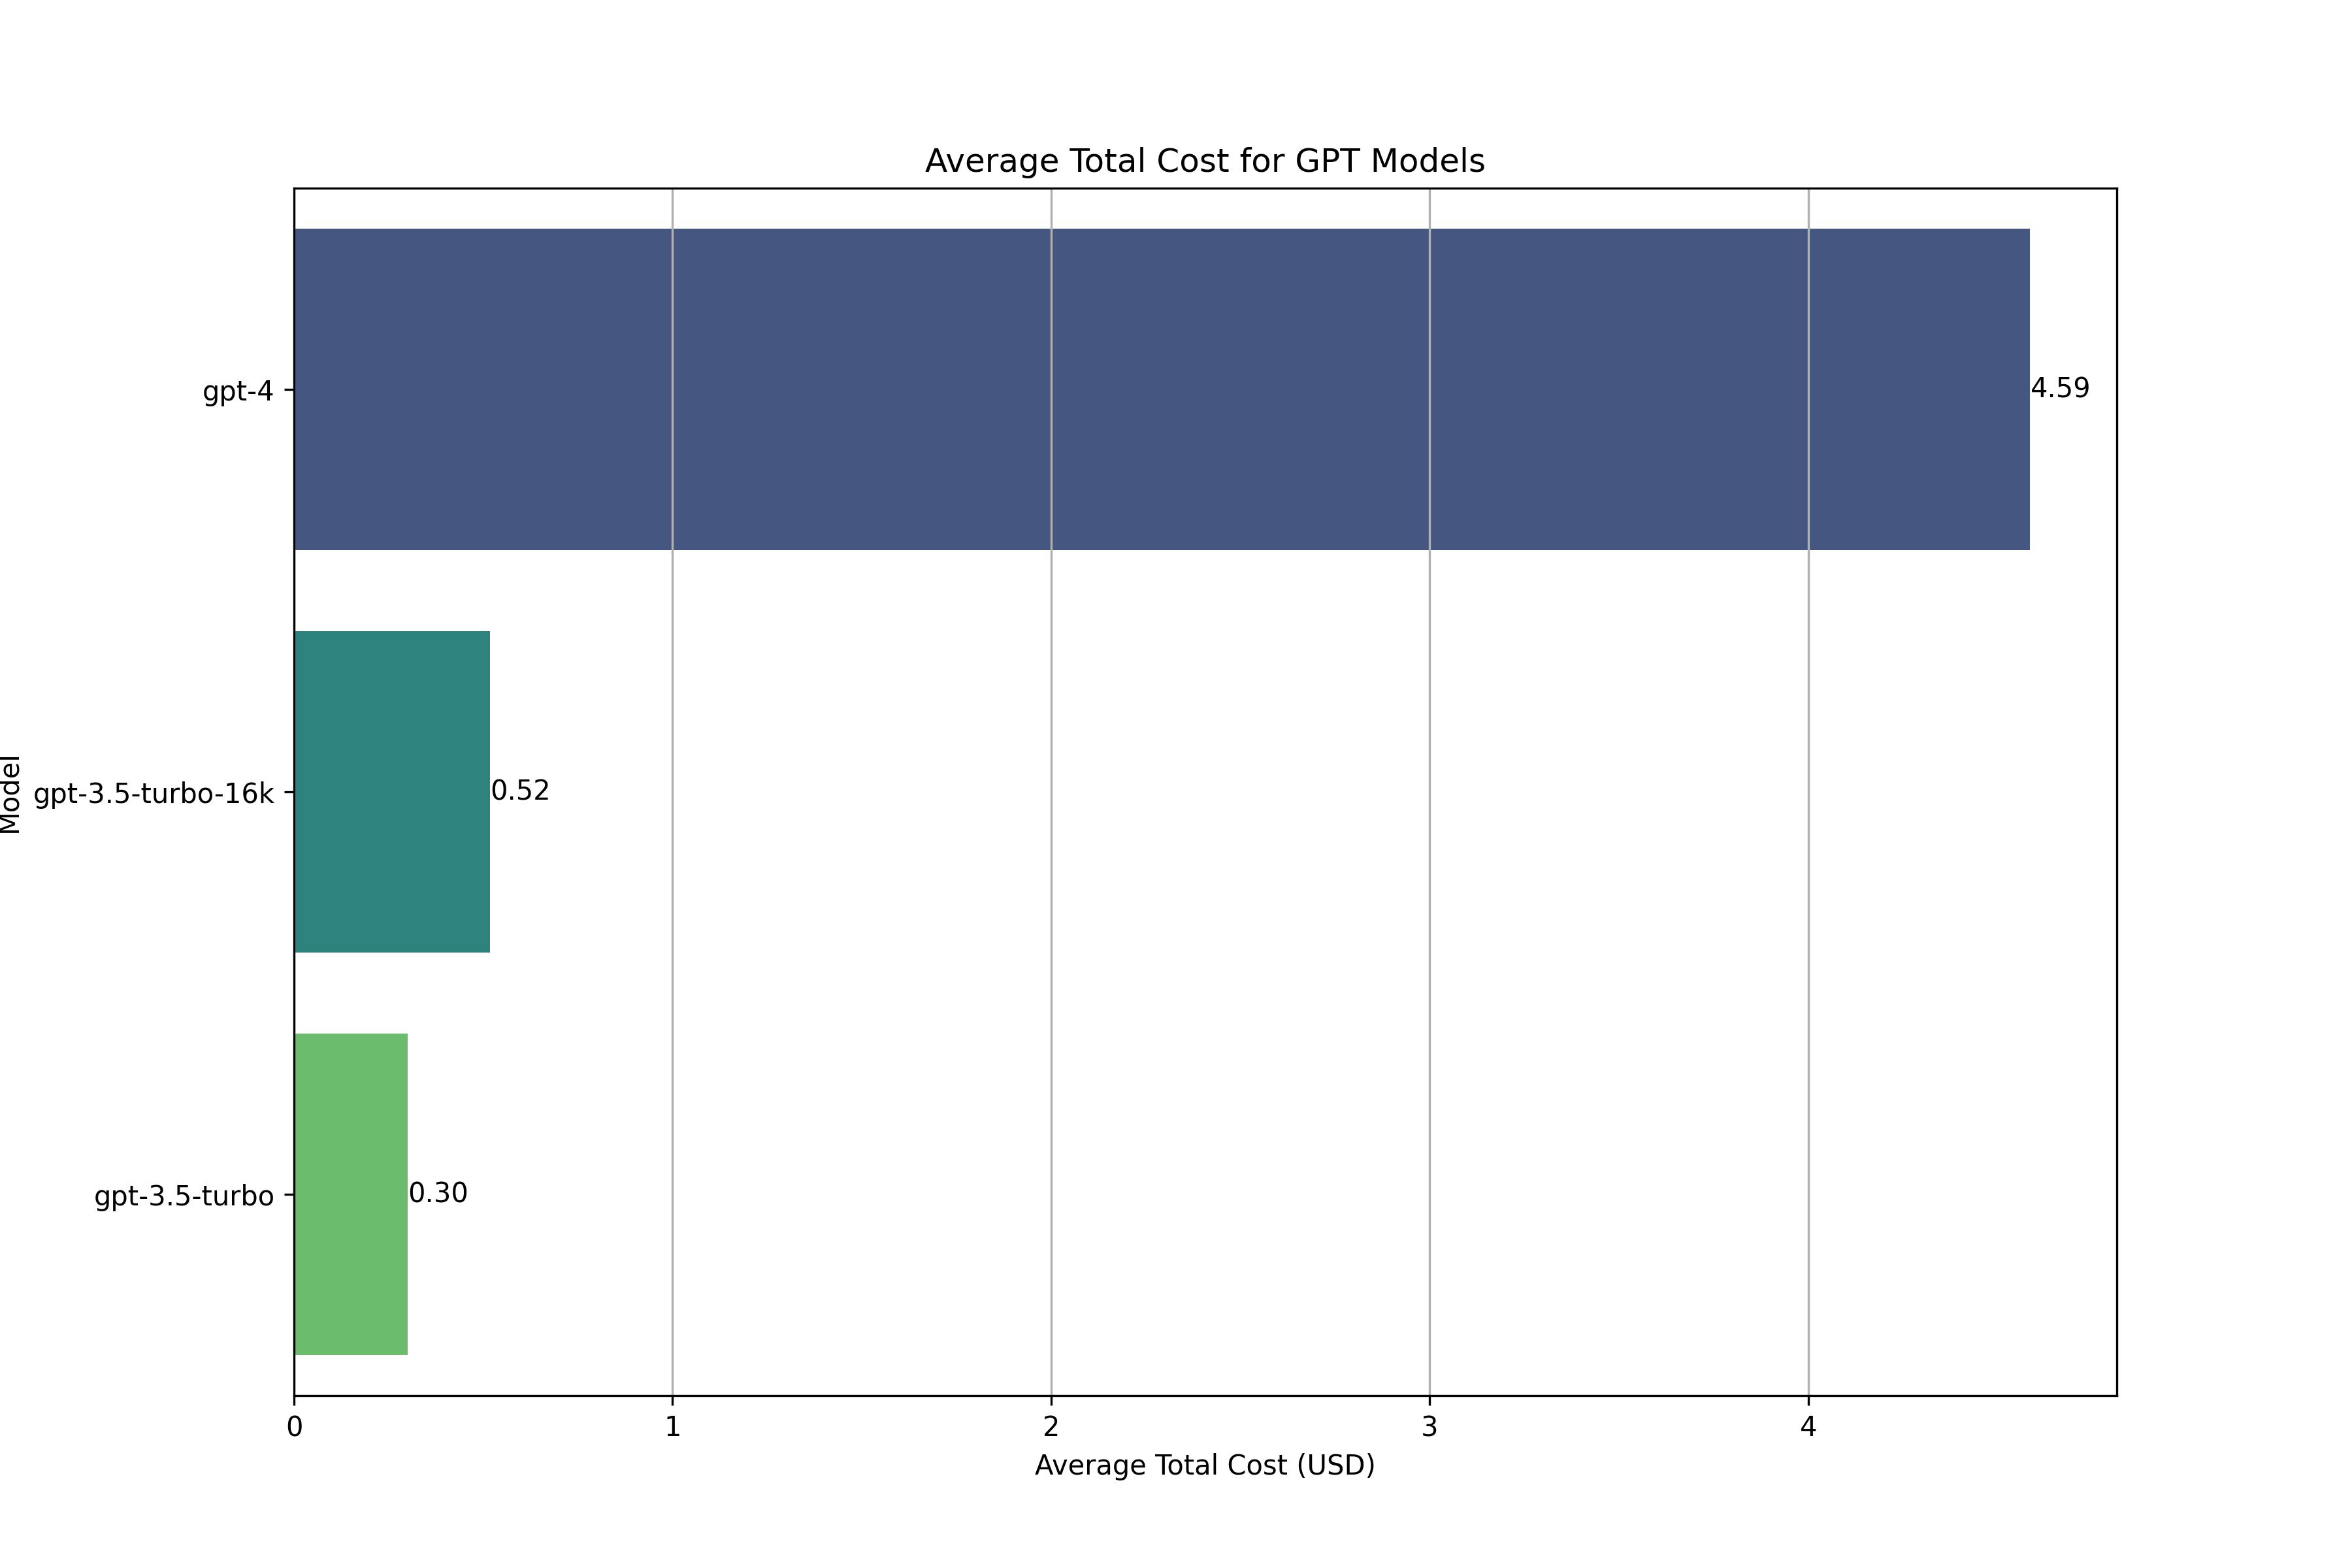
\includegraphics[width=11cm]{images/cost-gpt.png}
  \end{tabular}
  }
  \quad 
  \subfloat[Average Duration of Annotation]{
    \begin{tabular}{c}
  \hspace*{-1.5cm}
  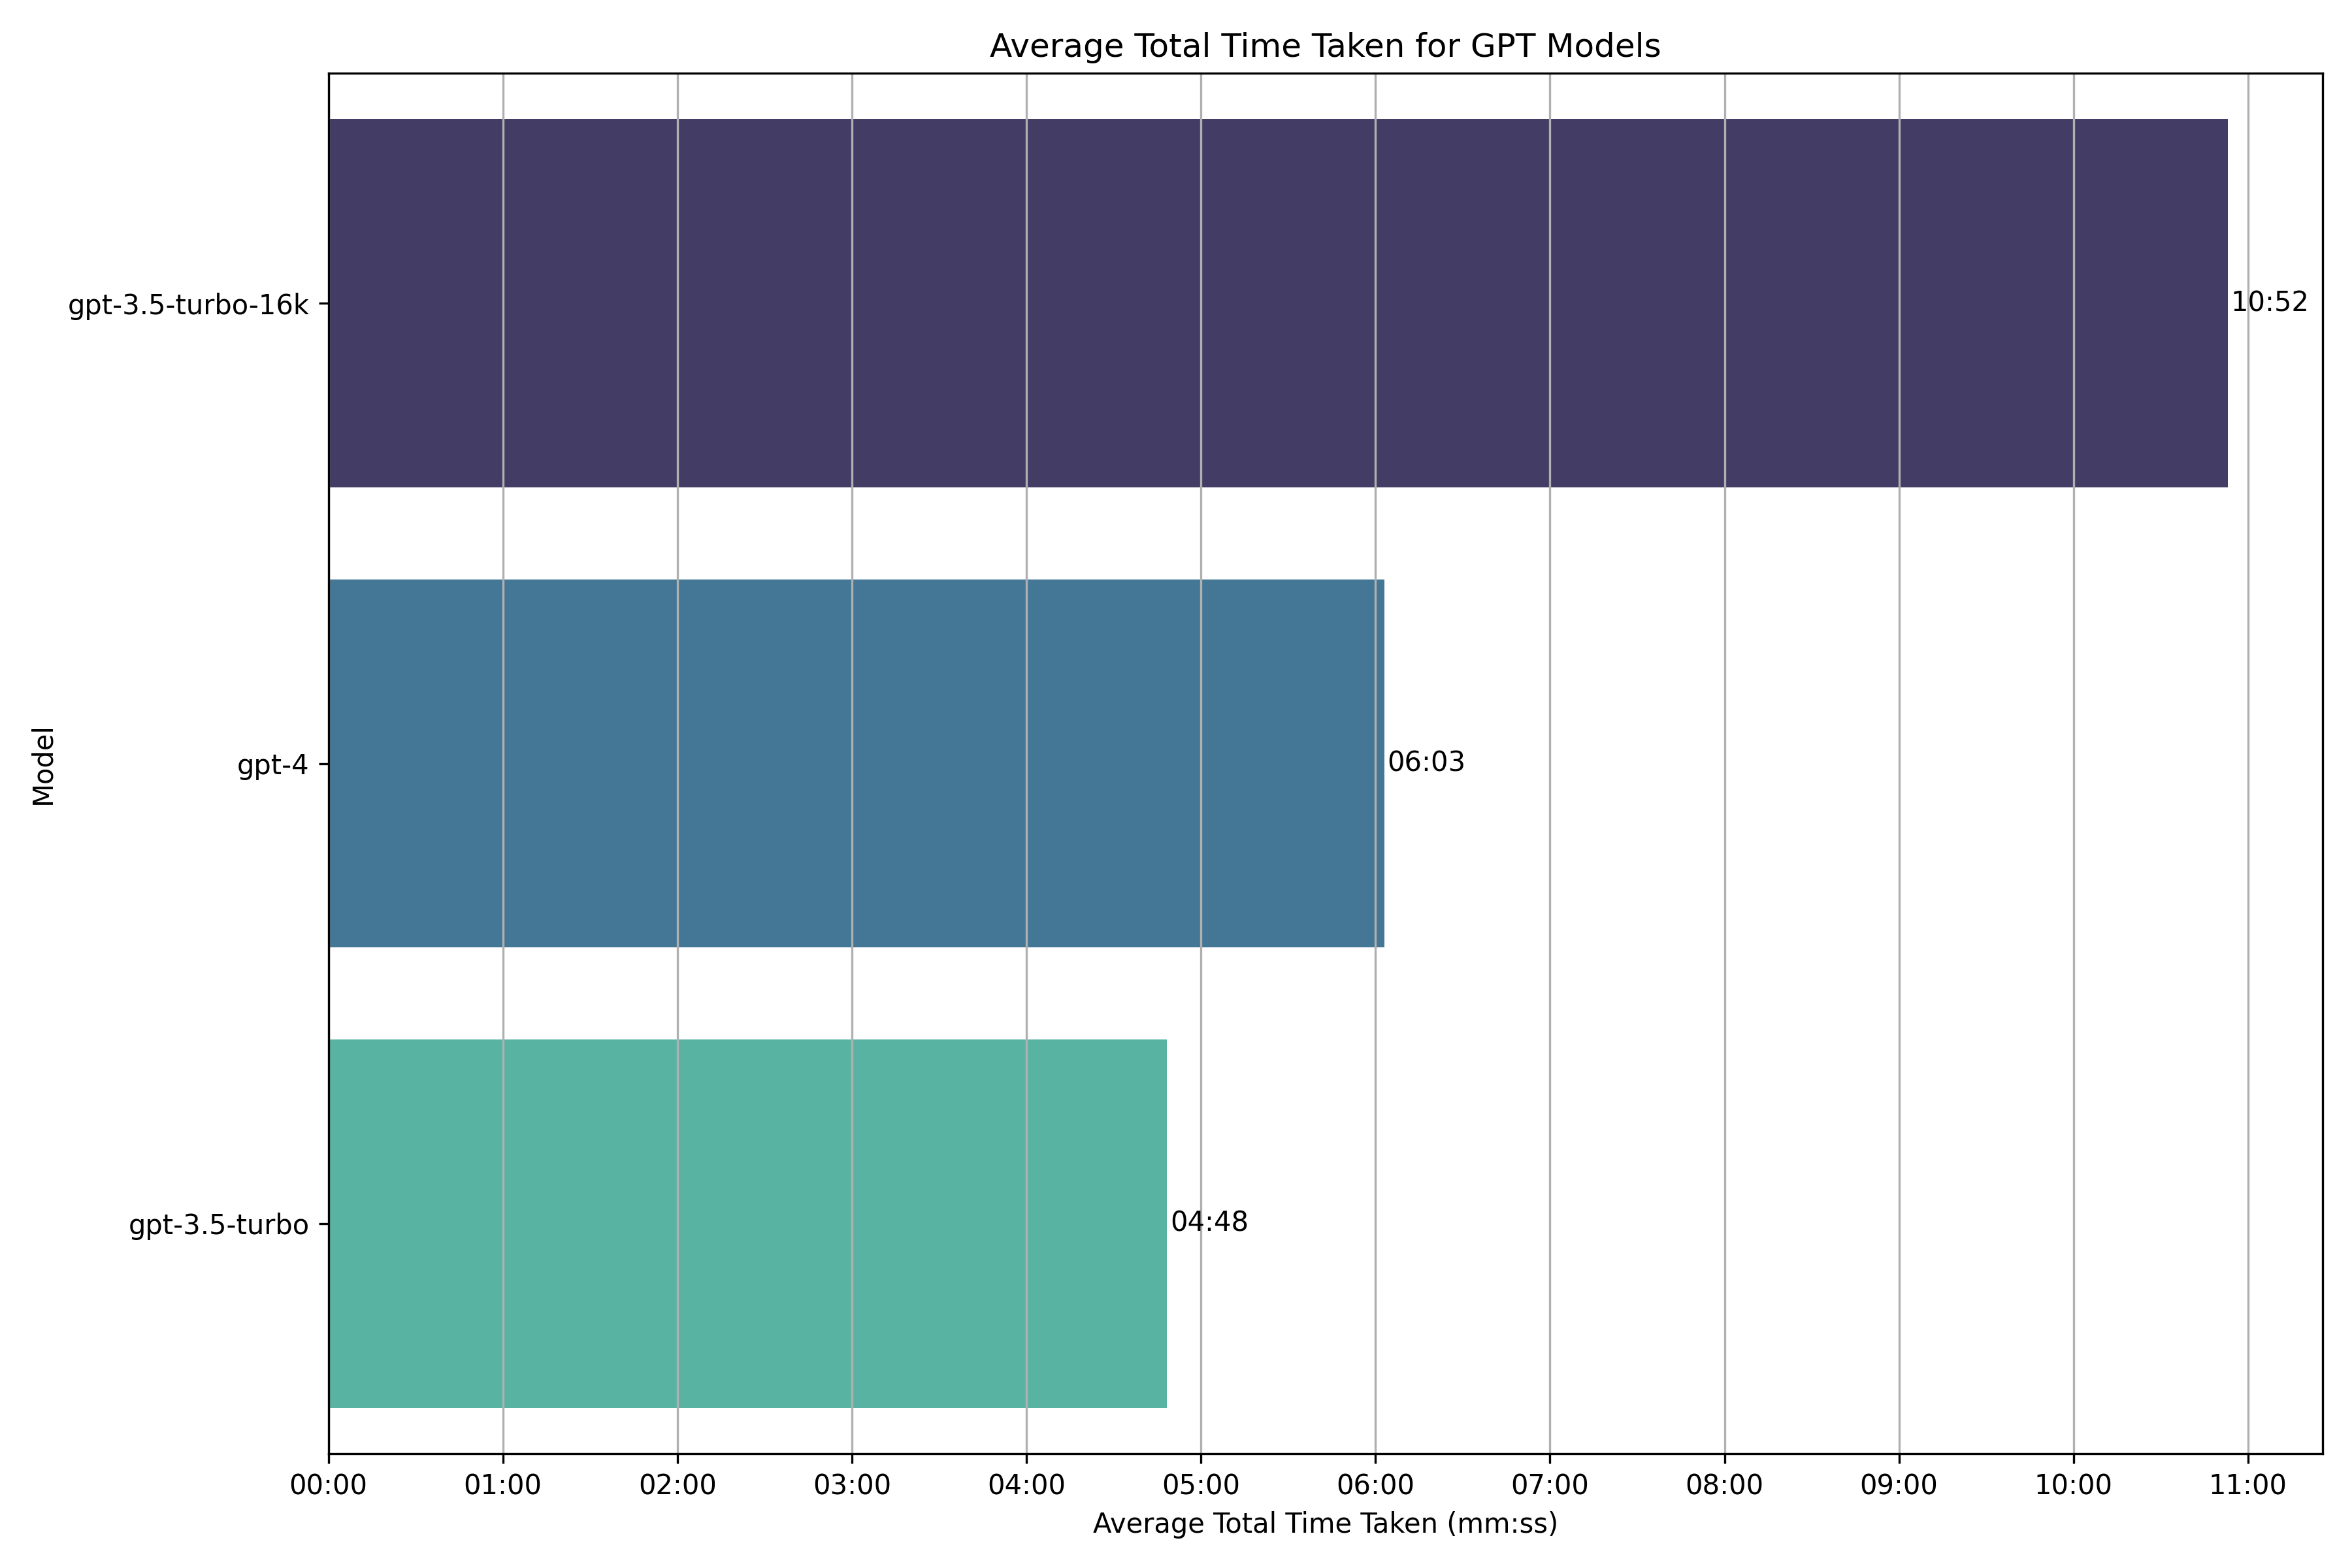
\includegraphics[width=10cm]{images/time-gpt.png}
  \end{tabular}
  }
  \caption[Cost Analysis]{Cost and Time Usage of Annotations}\label{fig:gpt-cost-anal}
\end{figure}

\begin{figure}[htpb]
  \centering
  \subfloat[Average Cost per 1000 Concept]{
    \begin{tabular}{c}
  %\hspace*{-.25cm}
  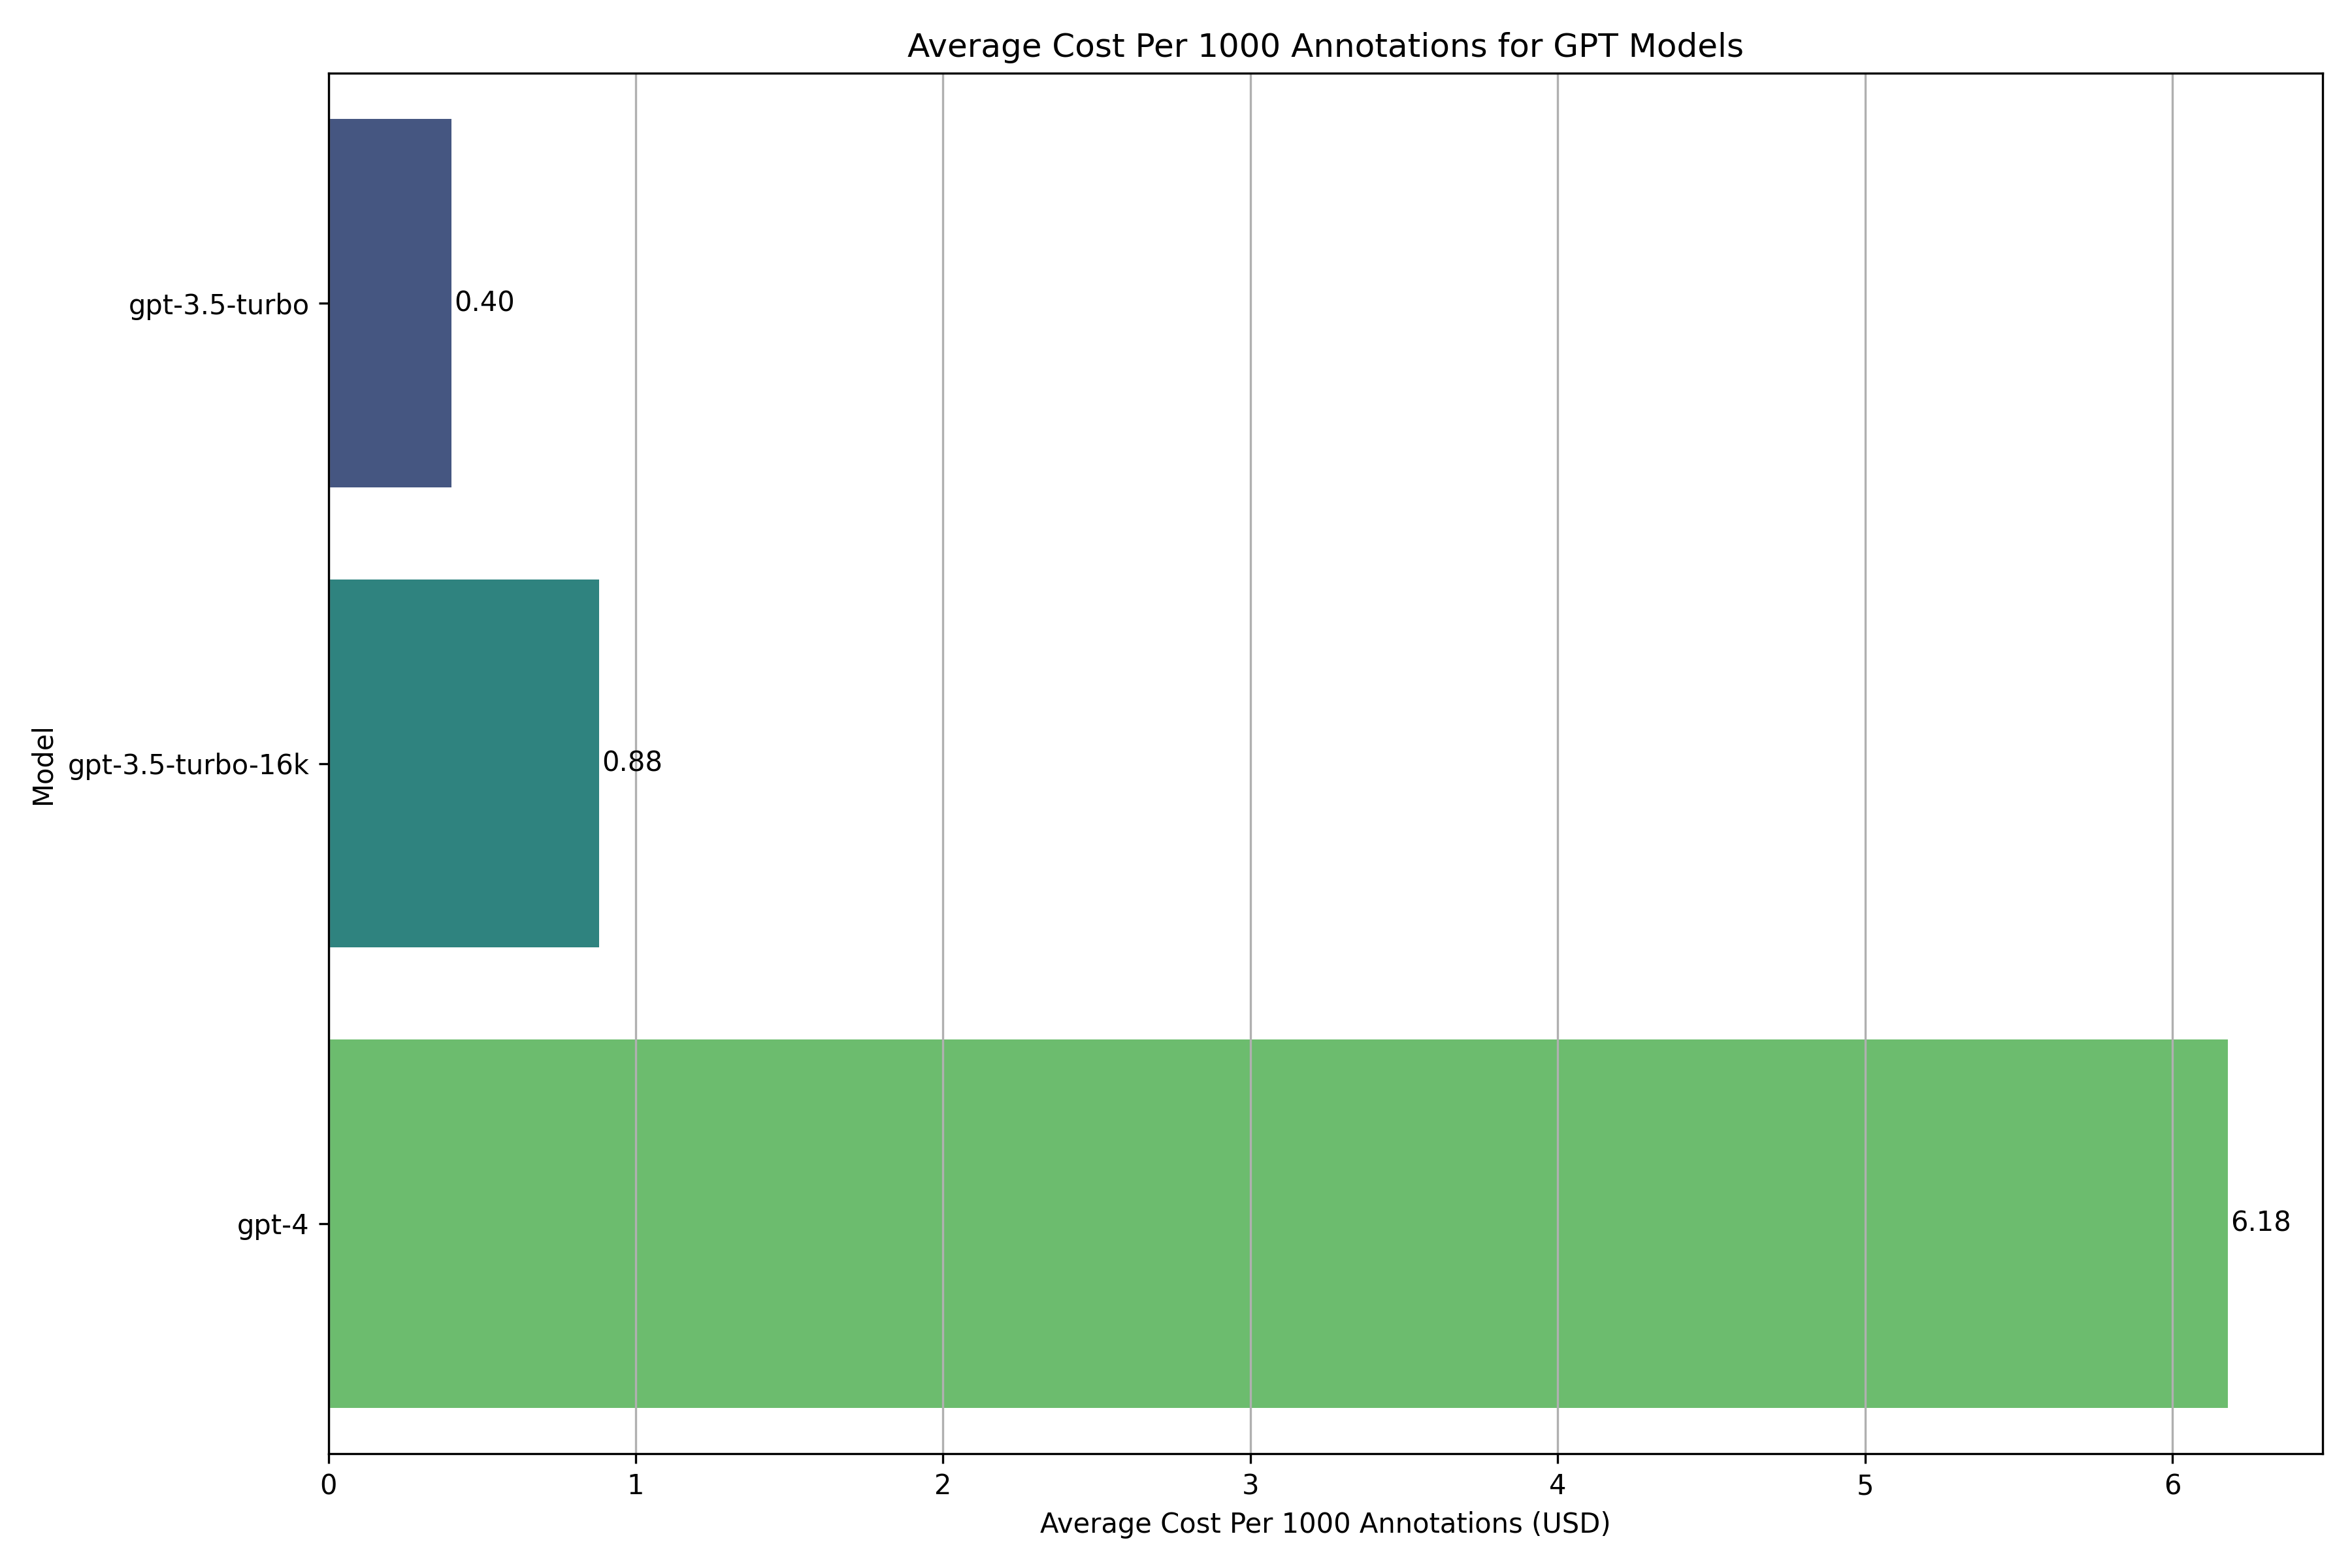
\includegraphics[width=11cm]{images/gpt-relative-cost.png}
  \end{tabular}
  }
  \quad 
  \subfloat[Average Duration per Concept]{
    \begin{tabular}{c}
  %\hspace*{-1.5cm}
  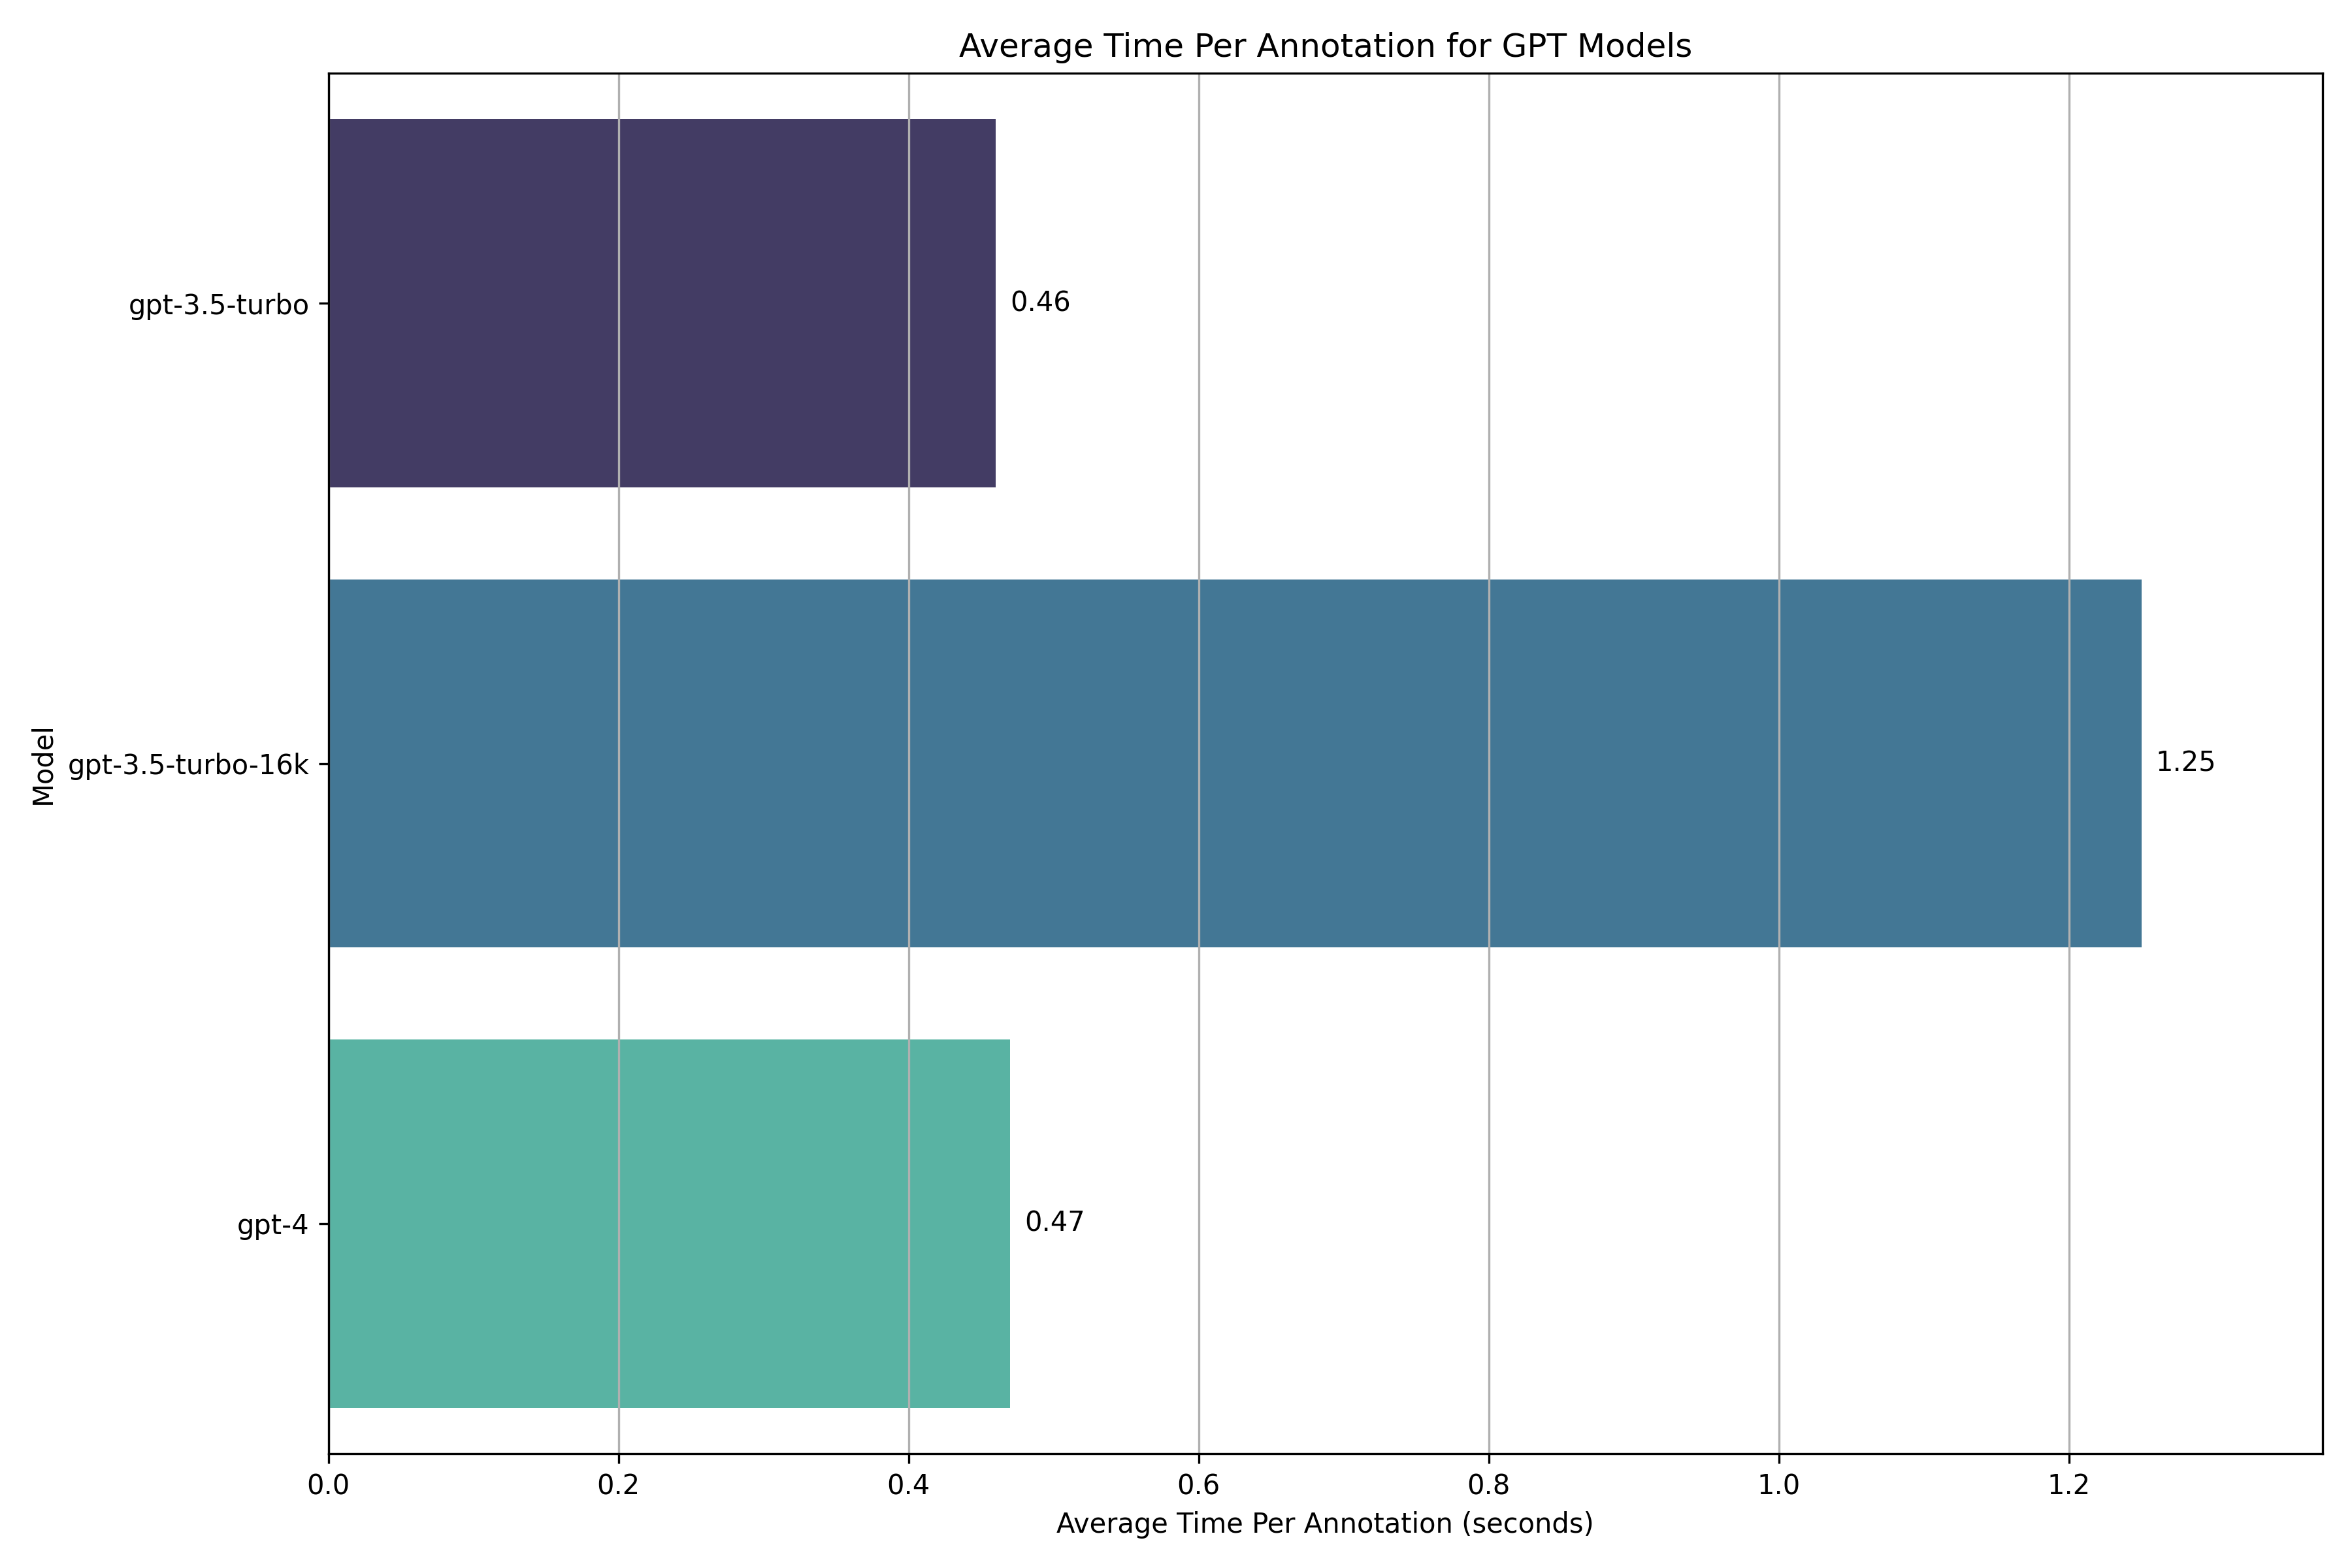
\includegraphics[width=10cm]{images/gpt-relative-time.png}
  \end{tabular}
  }
  \caption[Time Cost Analysis]{Cost and Time Usage of Automation}\label{fig:gpt-relative-cost}
\end{figure}

\begin{figure}[htpb]
  \centering
  \begin{tabular}{c}
  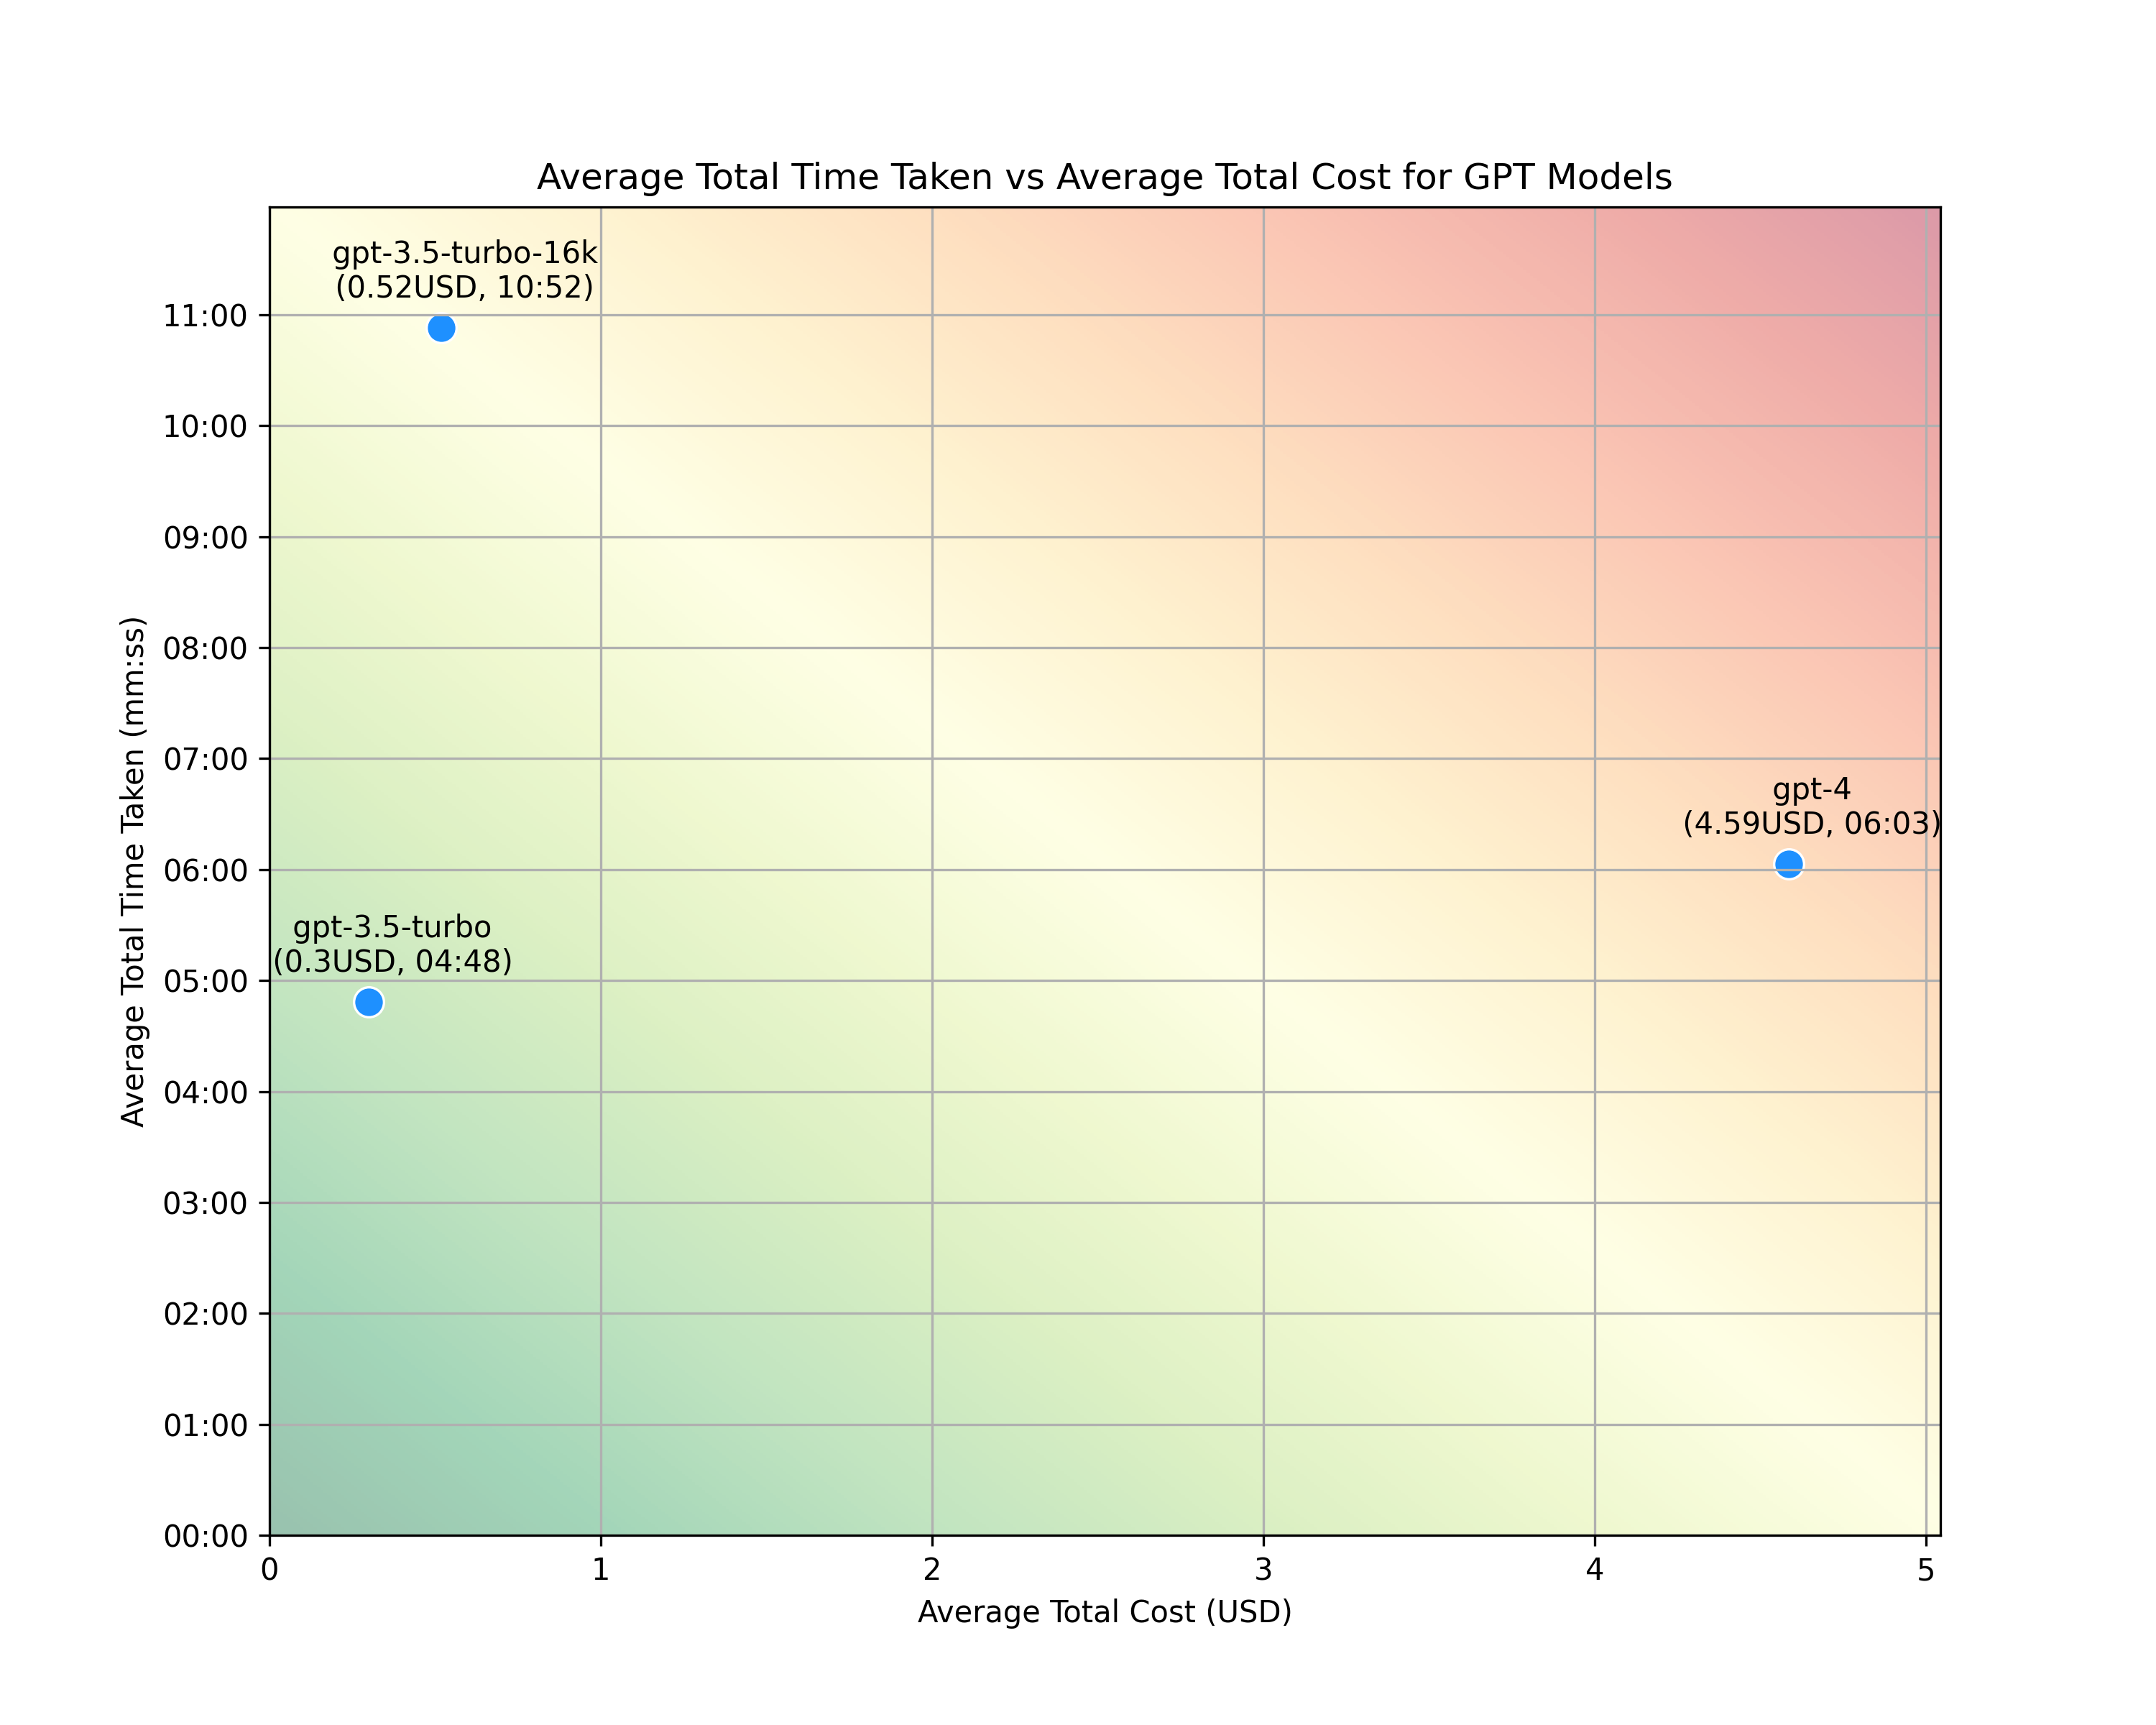
\includegraphics[width=14cm]{images/gpt-time-v-cost.png}
  \end{tabular}
  \caption[Cost vs Time]{Scatter Plot of Average Cost vs Time Taken}\label{fig:gpt-time-v-cost}
\end{figure}


\section{Open Souce LLMs}

We then scrutinised the annotations generated by OpenSource Models. We used a smaller subset of 7 papers from the 40 generated by \citet{asakura2022building} as the ground truth for this analysis. Then, we employed it to generate dictionaries and annotations for all these papers. The Open Source models varied in terms of their performance drastically. Among the two models we evaluated, Vicuna-33b lagged noticeably behind GPT models in performance. This outcome is expected because Vicuna-33b operates on a 33-billion parameter architecture. However, it is noteworthy that a scale model still demonstrates a formula grounding capability.

Conversely, StableBeluga2 exhibited remarkable performance, nearly matching that of GPT-4. This is particularly impressive, considering StableBeluga2 operates on a 70-billion parameter framework, while GPT-4 is rumoured to have a staggering 1.8 trillion parameters. Moreover, StableBeluga2 consistently outperformed GPT-3.5 across multiple metrics. This superior performance is likely attributable to the specialised nature of StableBeluga2, designed as an "instruct" model, in contrast to GPT models that are general-purpose chat models not explicitly optimised for formula grounding.

\subsection{CoNLL Score}

Vicuna-33b struggled in several cases, even scoring zero in one instance, hinting at its inability to generate any meaningful dictionary for that paper. StableBeluga2, on the other hand, aptly managed to deliver performances that stood almost on par with GPT Models as illustrated in Figure \ref{fig:open-source-conll}. Despite this, GPT models maintained a discernible edge in disambiguation capabilities over their open-source counterparts. This advantage is likely attributable to the extensive training that GPT models undergo.

\begin{figure}[htpb]
  \centering
  \begin{tabular}{c}
  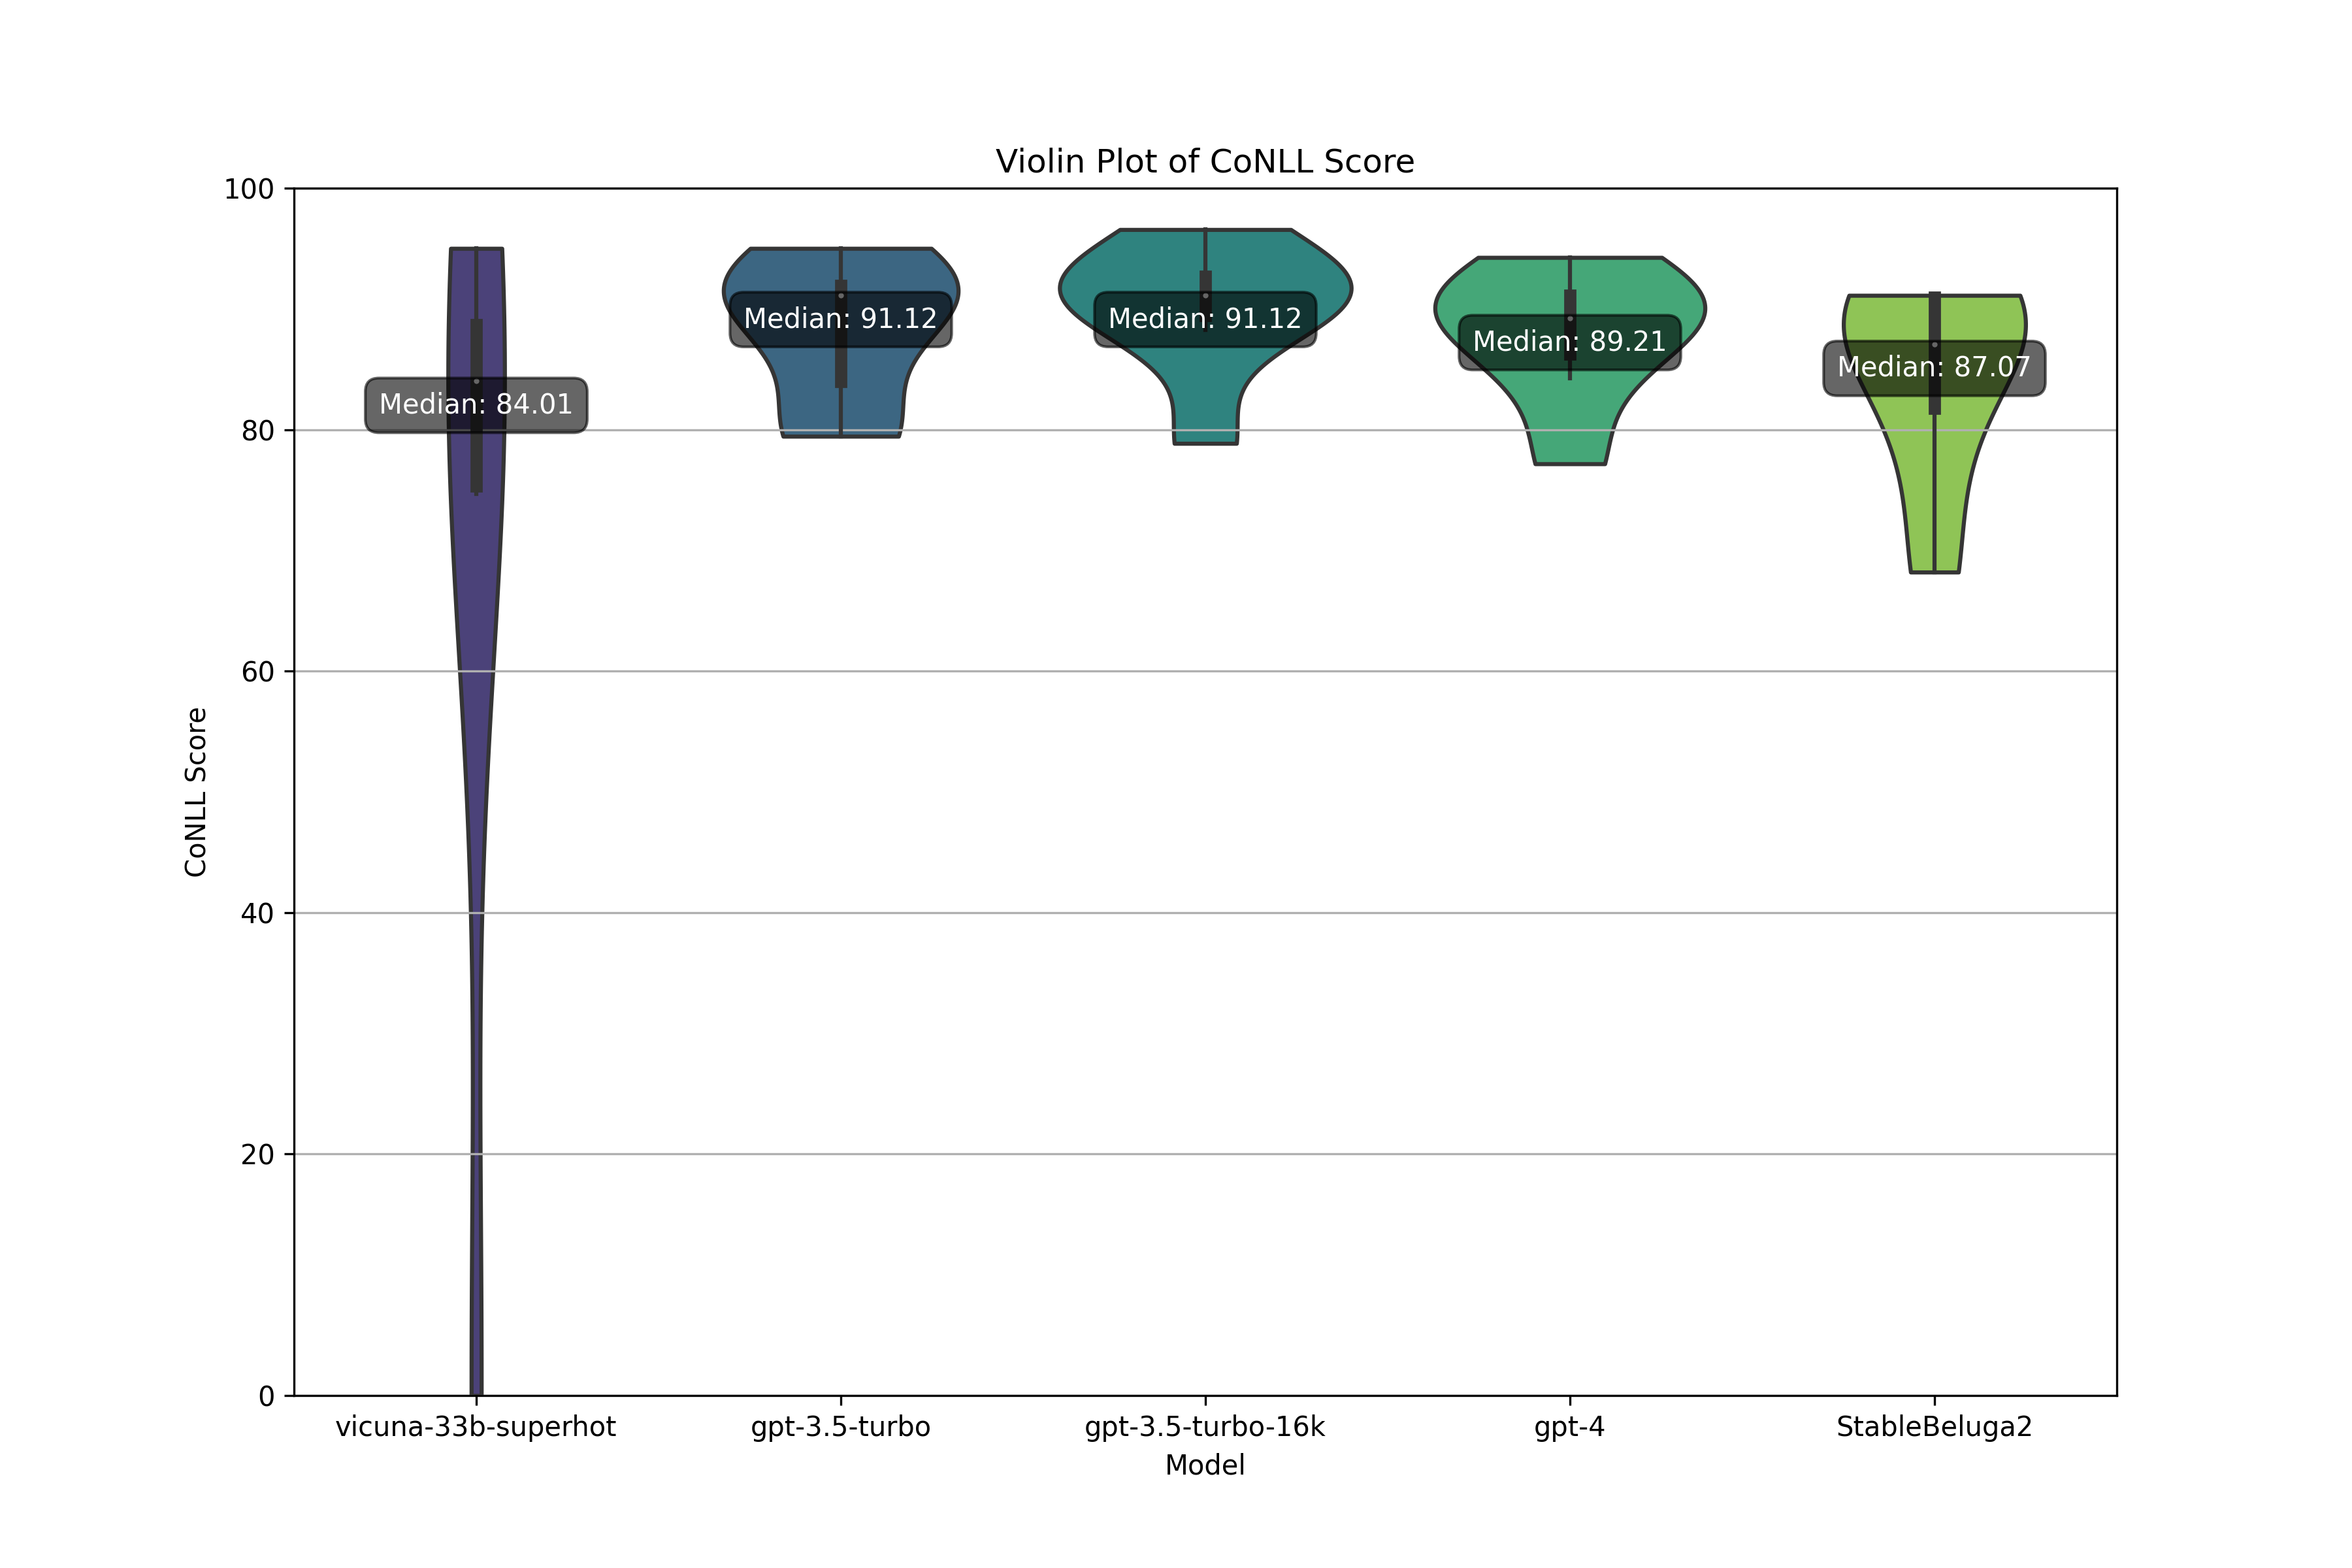
\includegraphics[width=14cm]{images/open-conll-score.png}
  \end{tabular}
  \caption[CoNLL Score Open Source]{Violin Plot of the CoNLL scores using all 5 models}\label{fig:open-source-conll}
\end{figure}

\subsection{Coverage of Annotation}

Once again, vicuna-33b faced challenges in providing complete coverage for one paper, resulting in a score of zero. StableBeluga2, achieving performances comparable to GPT Models, presents an insightful contrast as further evidenced in Figure \ref{fig:open-coverage}. Despite this isolated setback for Vicuna-33b, its performance generally remains subpar compared to its more advanced counterparts. 

\begin{figure}[htpb]
  \centering
  \begin{tabular}{c}
  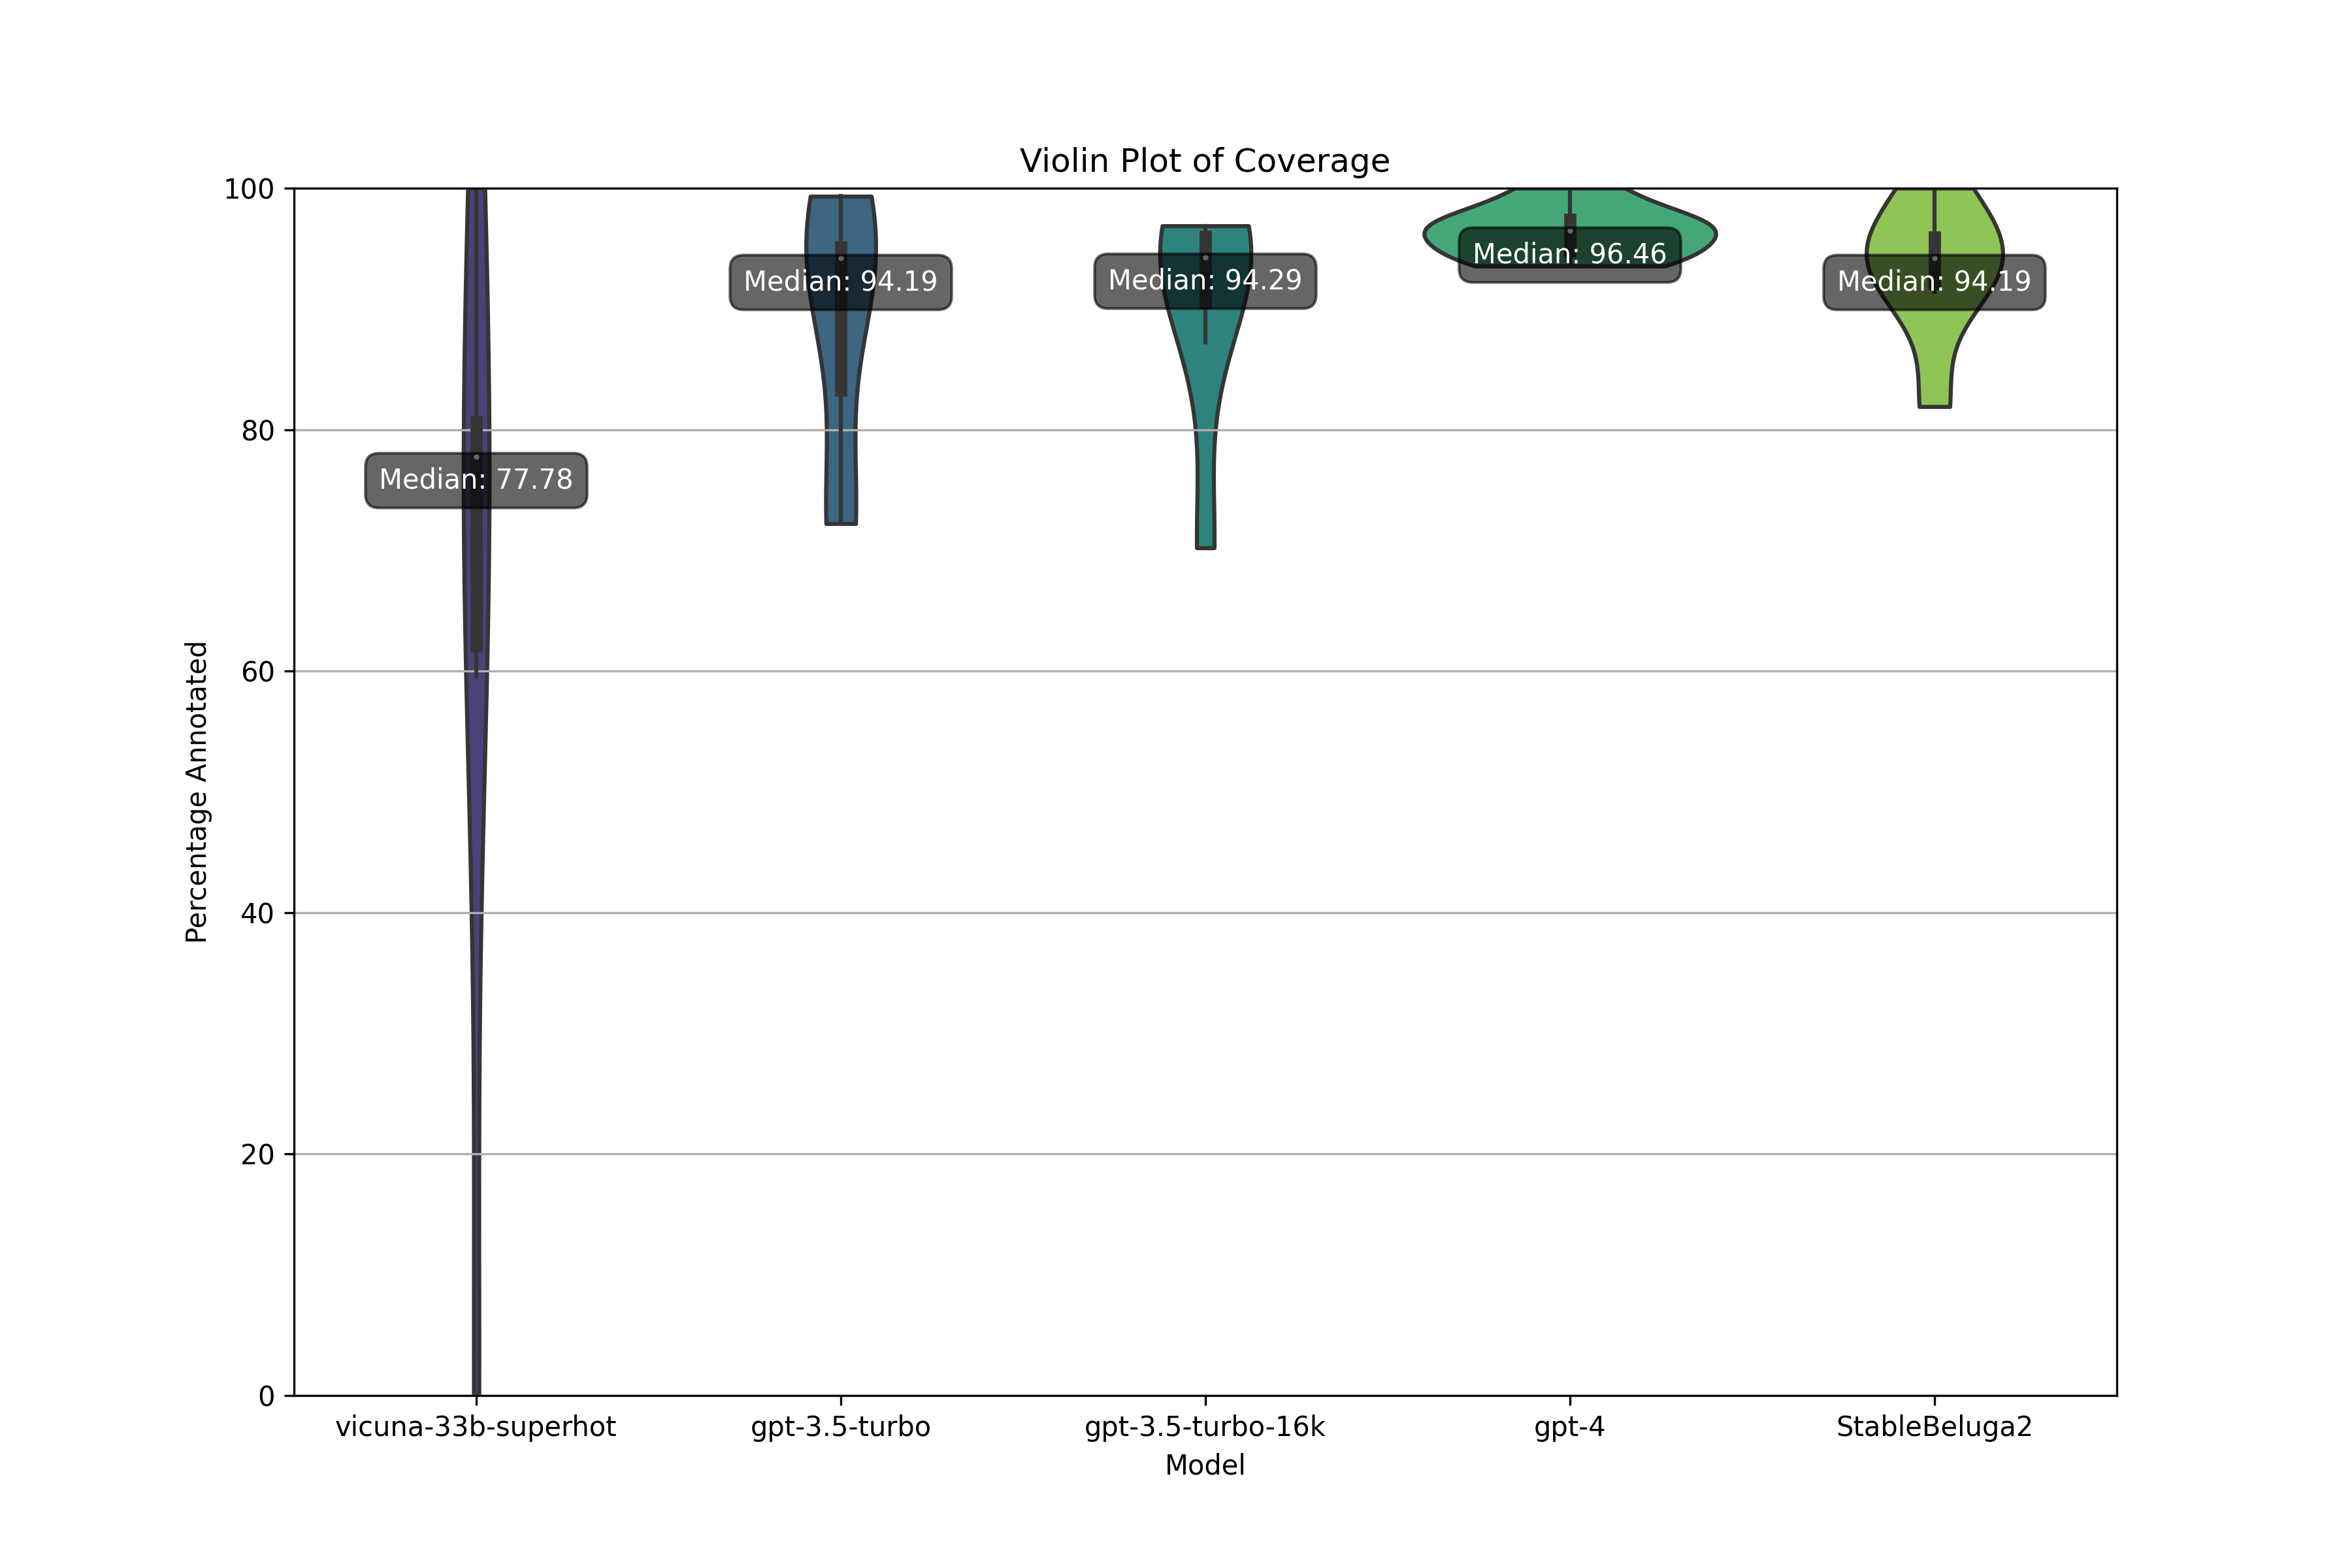
\includegraphics[width=14cm]{images/open-coverage.png}
  \end{tabular}
  \caption[Open Source Coverage]{Violin Plot of the coverage of the papers annotated}\label{fig:open-coverage}
\end{figure}

\subsection{Semantic Accuracy}

Semantic accuracy functions as the cornerstone of our comparative study. Due to the labour-intensive nature of manual evaluation, we selected a subset of six papers for this purpose. StableBeluga2, an Open Source LLM, beats GPT-3.5 entirely yet could not surpass GPT-4, which deserves mention due to the unmatched complexity and sophistication of GPT-4's architecture. As detailed in Figure \ref{fig:open-semantic}, the semblance between the performance of StableBeluga2 and GPT models reinforces this open-source model's potential in accurately understanding and reflecting the context of scientific papers. Vicuna-33b's performance was notably lacklustre, a limitation likely attributable to its smaller model size.

\begin{figure}[htpb]
  \centering
  \begin{tabular}{c}
  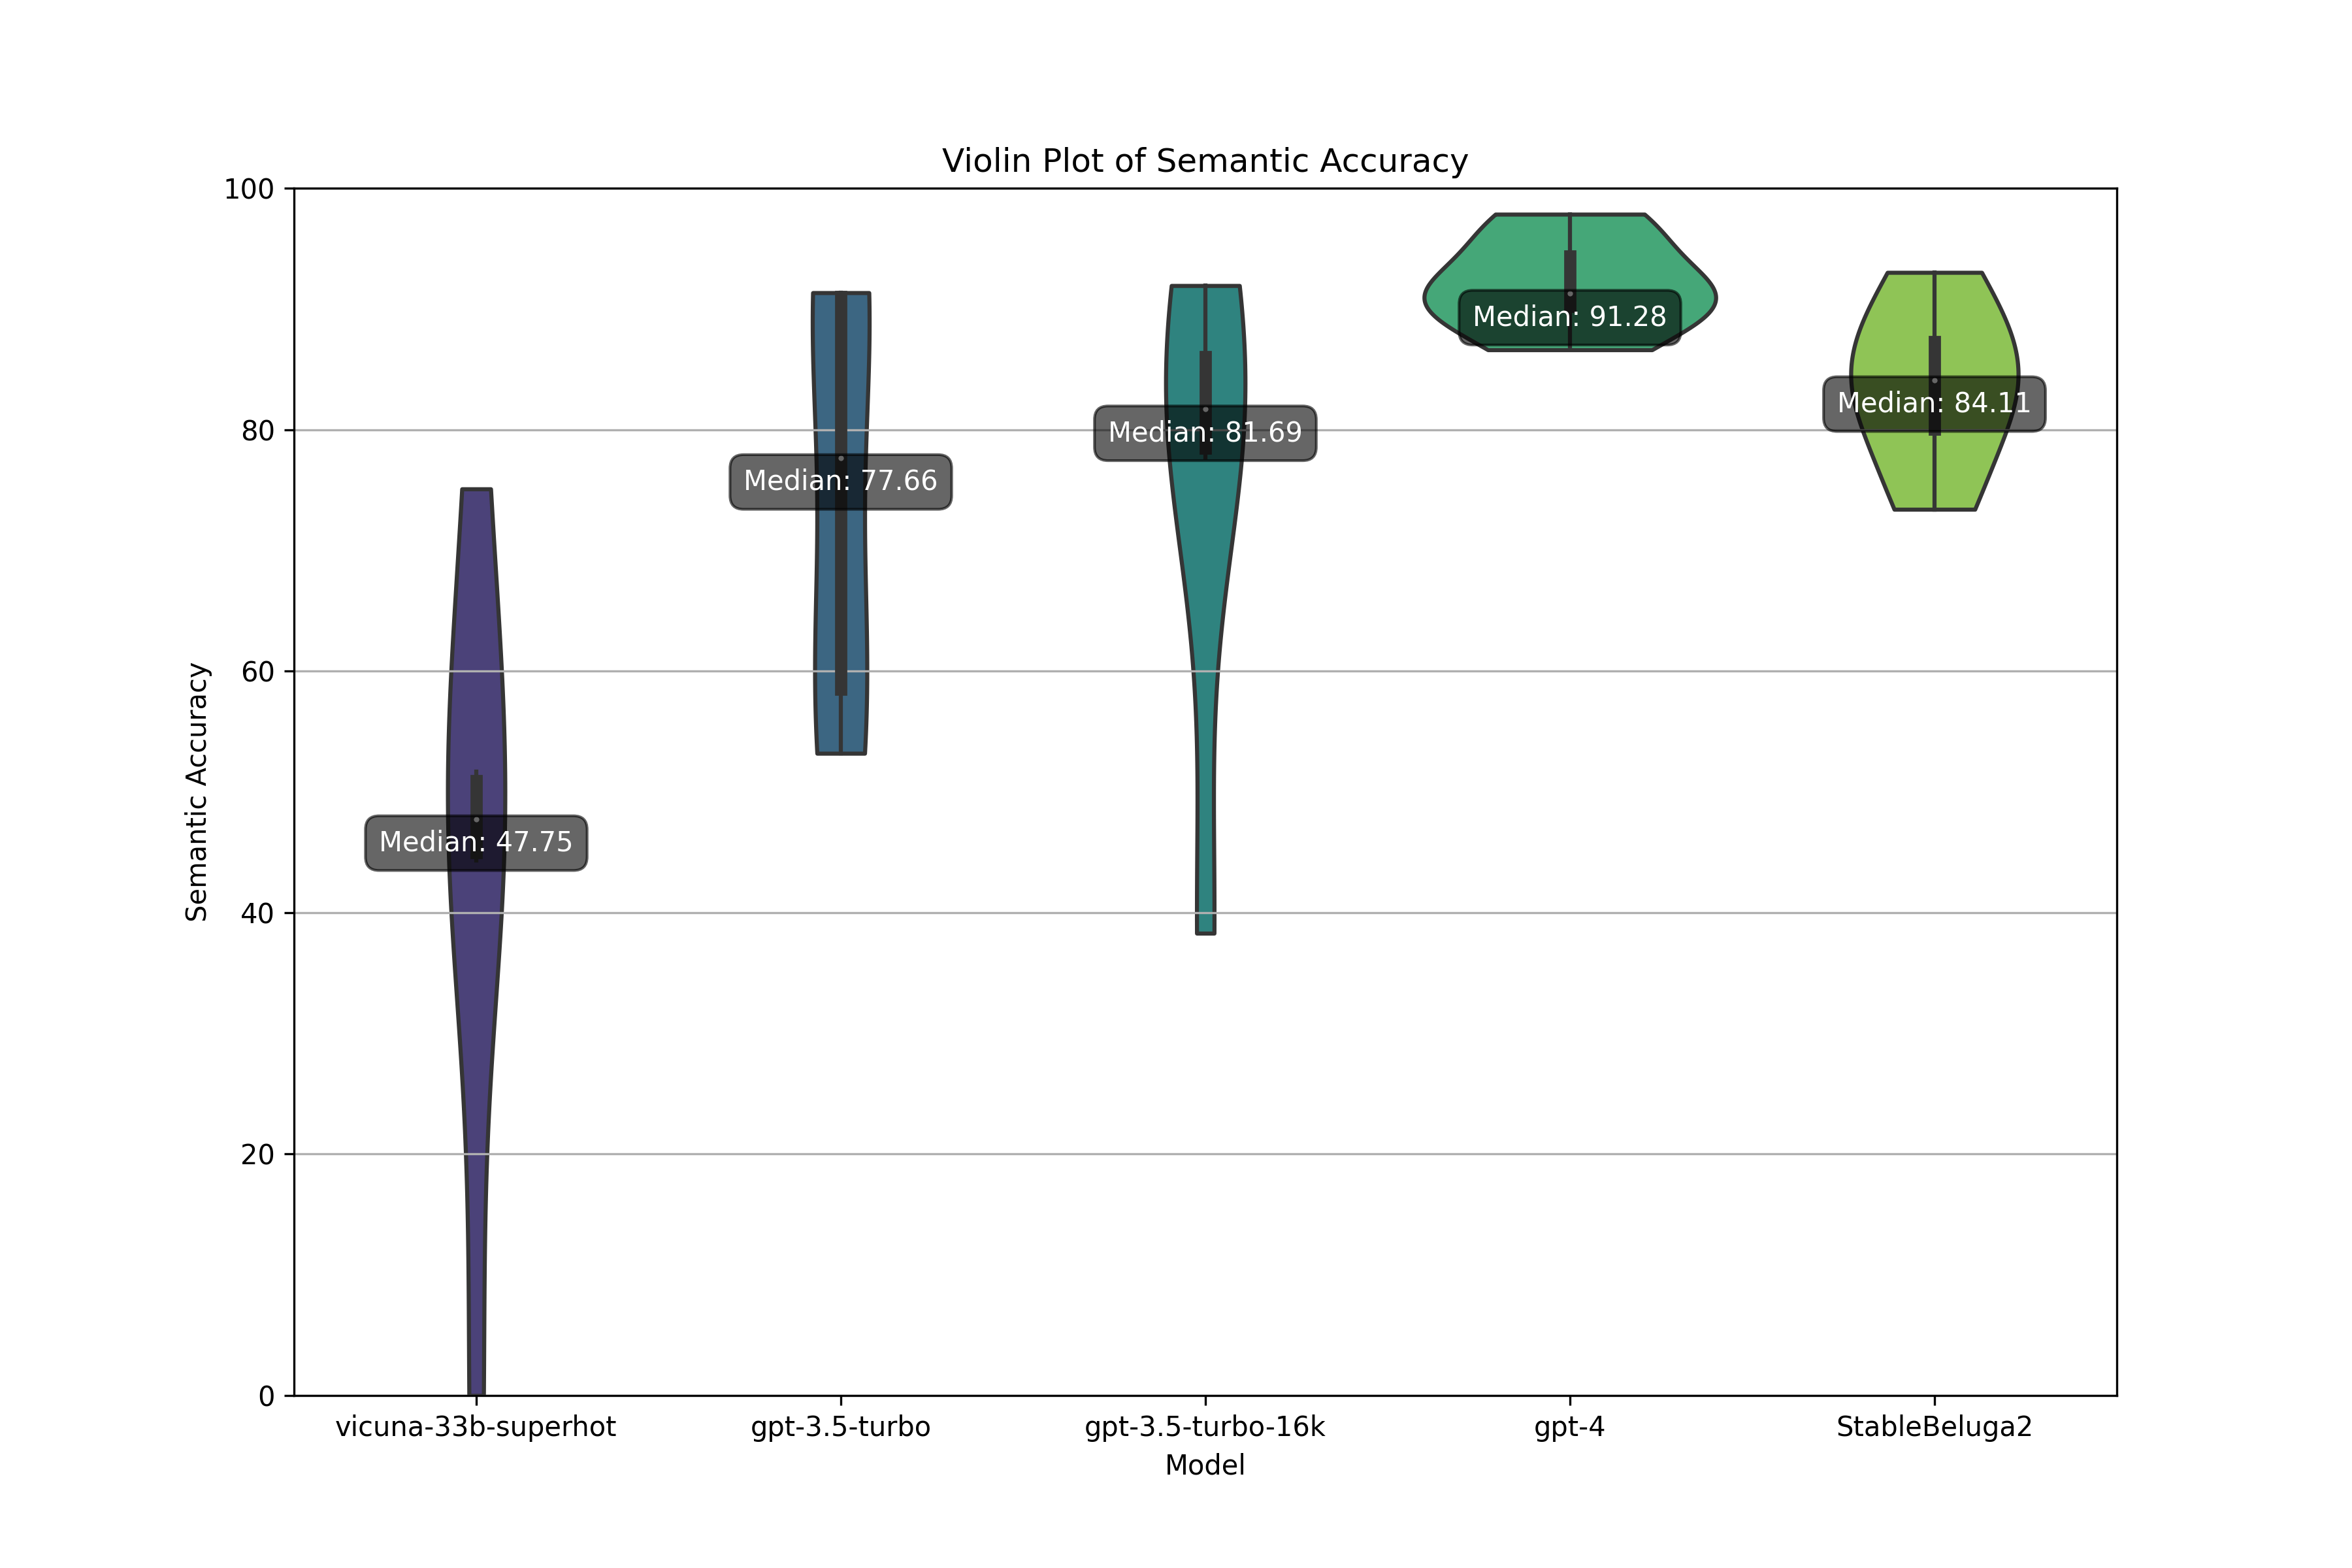
\includegraphics[width=14cm]{images/open-semantic.png}
  \end{tabular}
  \caption[Semantic Accuracy]{Semantic Accuracy Scores from all the 5 models}\label{fig:open-semantic}
\end{figure}

\subsection{Running Time and Costs}

Given the distinctive operational requirements of open-source models, the computation of time and cost efficiencies differ from those of GPT models. Unlike GPT models, the cost for open-source models revolves around GPU runtime, and in our case, on the servers of \href{https://runpod.io}{runpod.io} and not token usage. The running time is visualised in Figure \ref{fig:open-runtime}. However, since the time taken here depends on the length of the paper, it is essential to compare the costs per annotation. This can be visualised in \ref{fig:open-relative-cost}. Because of cheaper hardware, the average run time of open-source LLMs was prolonged. On average, they were 5-10x slower. This is especially noticeable for StableBeluga2 as it is a Large LLM. The cost for the experiments can differ from person to person, as we had to pay for the GPU usage. If a person owns GPUs, it will be free of cost; however, regardless, we have visualised the cost we paid for annotations in Figure \ref{fig:open-cost}. It can also very well happen that the cost to use these GPUs is way higher than GPT. GPT-4 is significantly more expensive than all other models. vicuna-33b has a similar operating cost to GPT-3.5 but performs way worse. StableBeluga2, which performs better than GPT-3.5, costs 3x more than GPT-3.5 and 3x less than GPT-4.

\begin{figure}[htpb]
  \centering
  \begin{tabular}{c}
  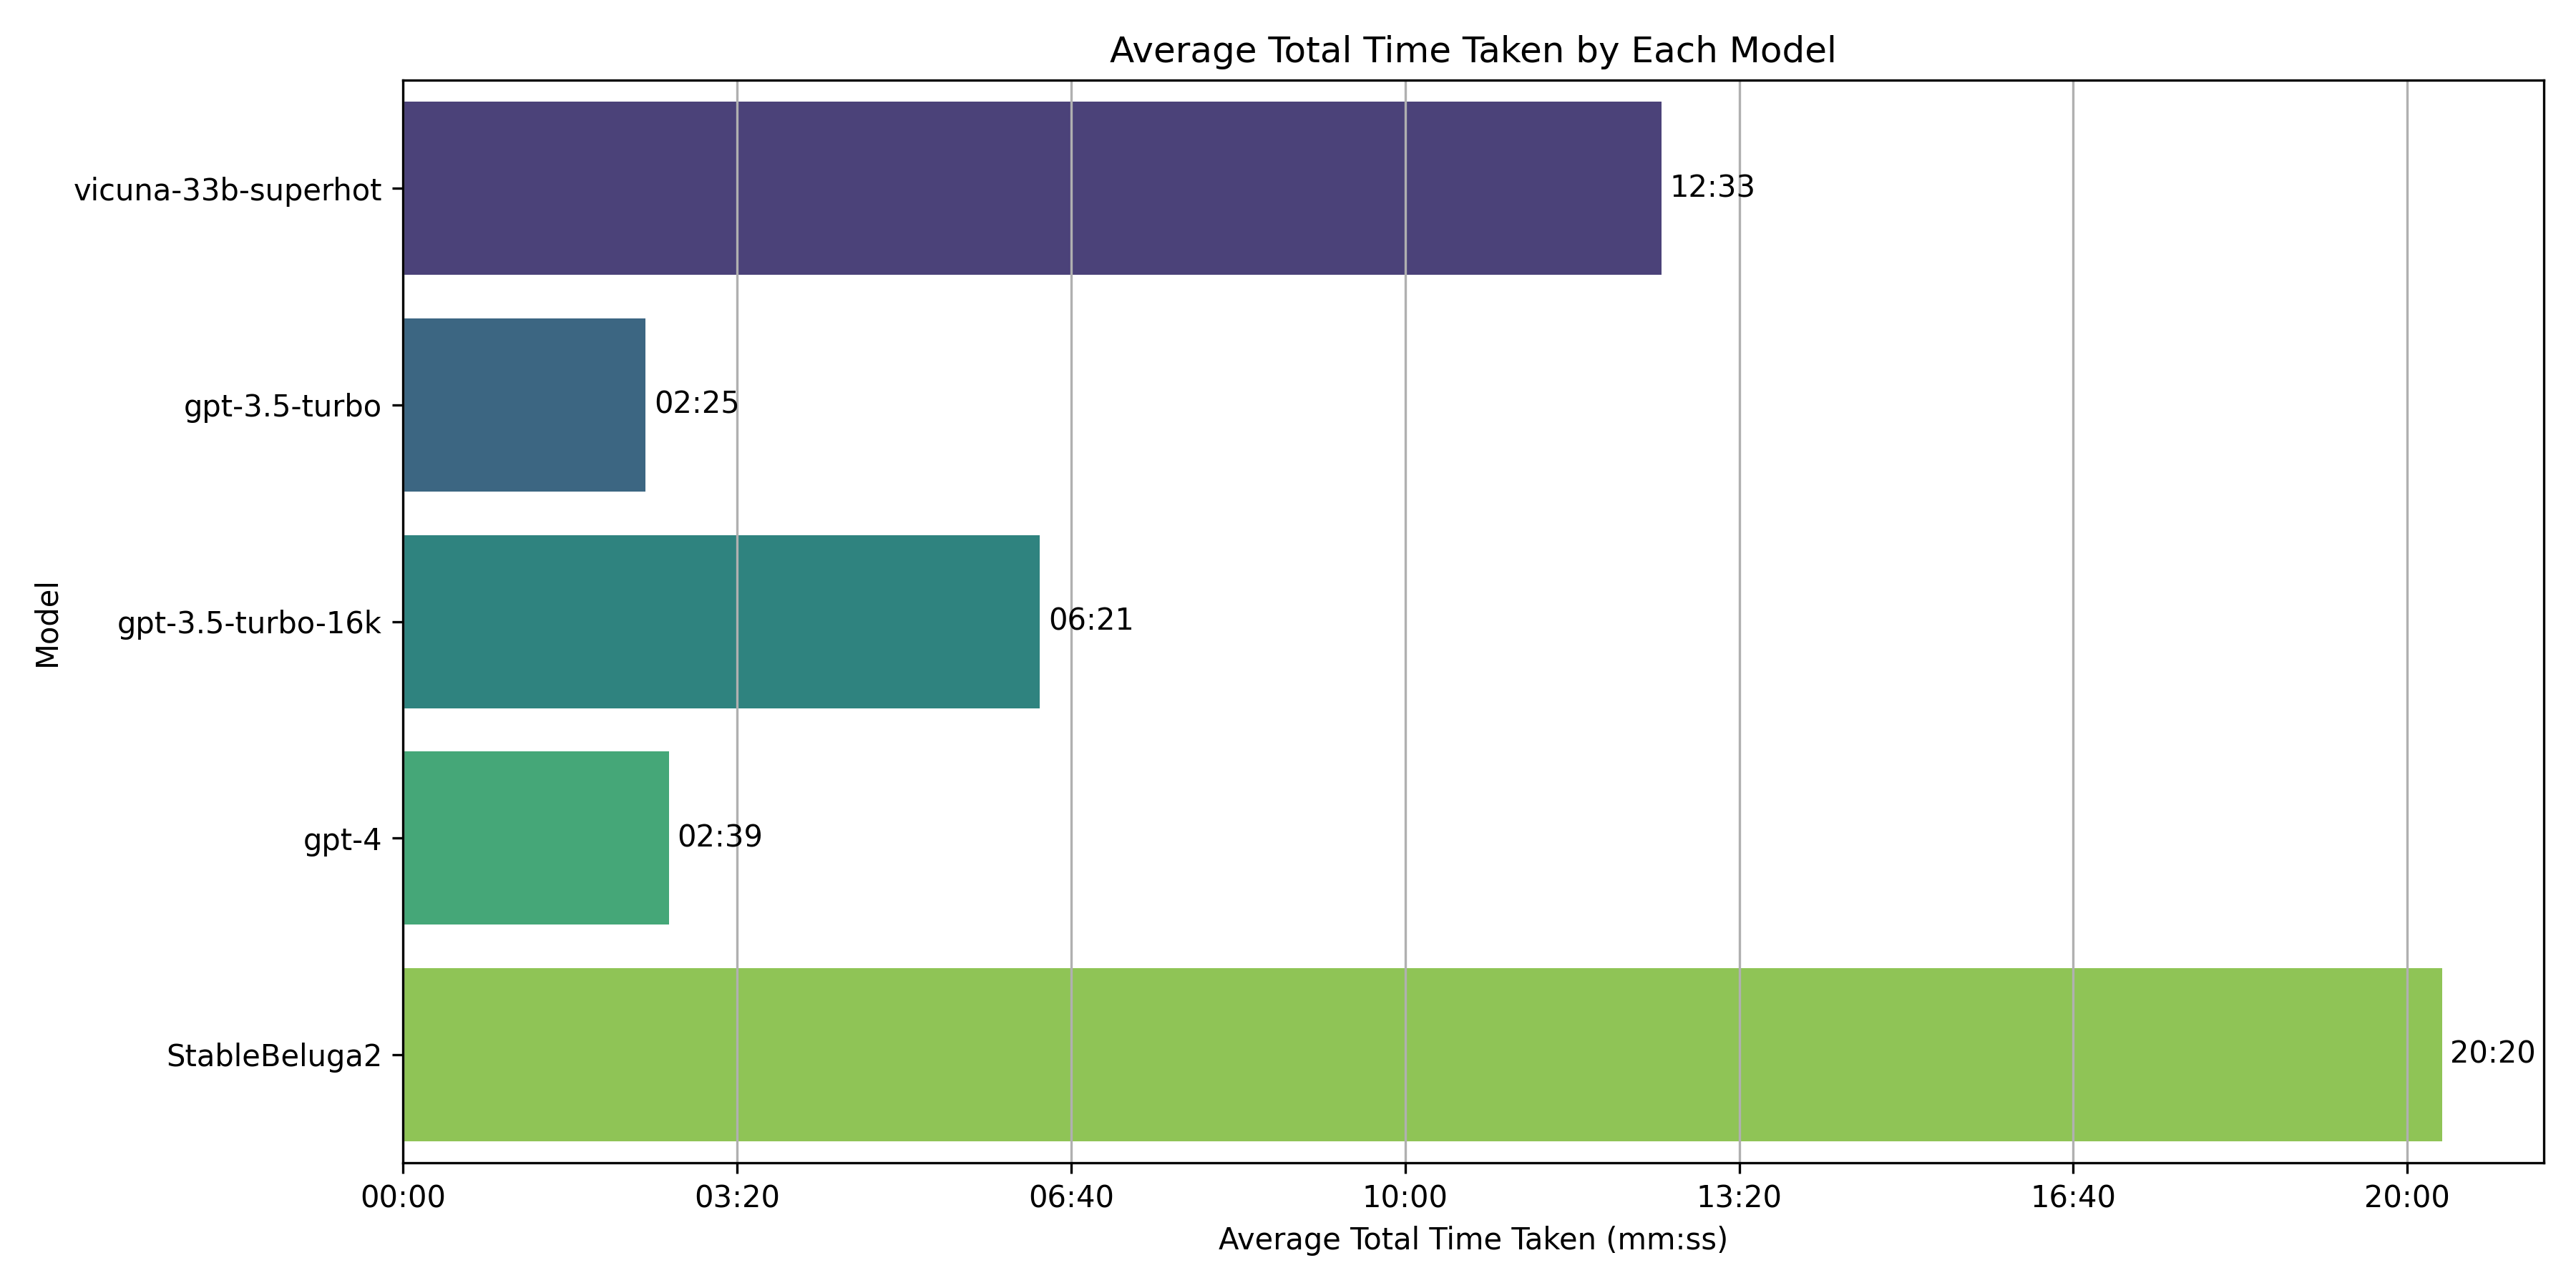
\includegraphics[width=14cm]{images/open-runtime.png}
  \end{tabular}
  \caption[Open Source Time]{Average Time Taken by all five models}\label{fig:open-runtime}
\end{figure}

\begin{figure}[htpb]
  \centering
  \begin{tabular}{c}
  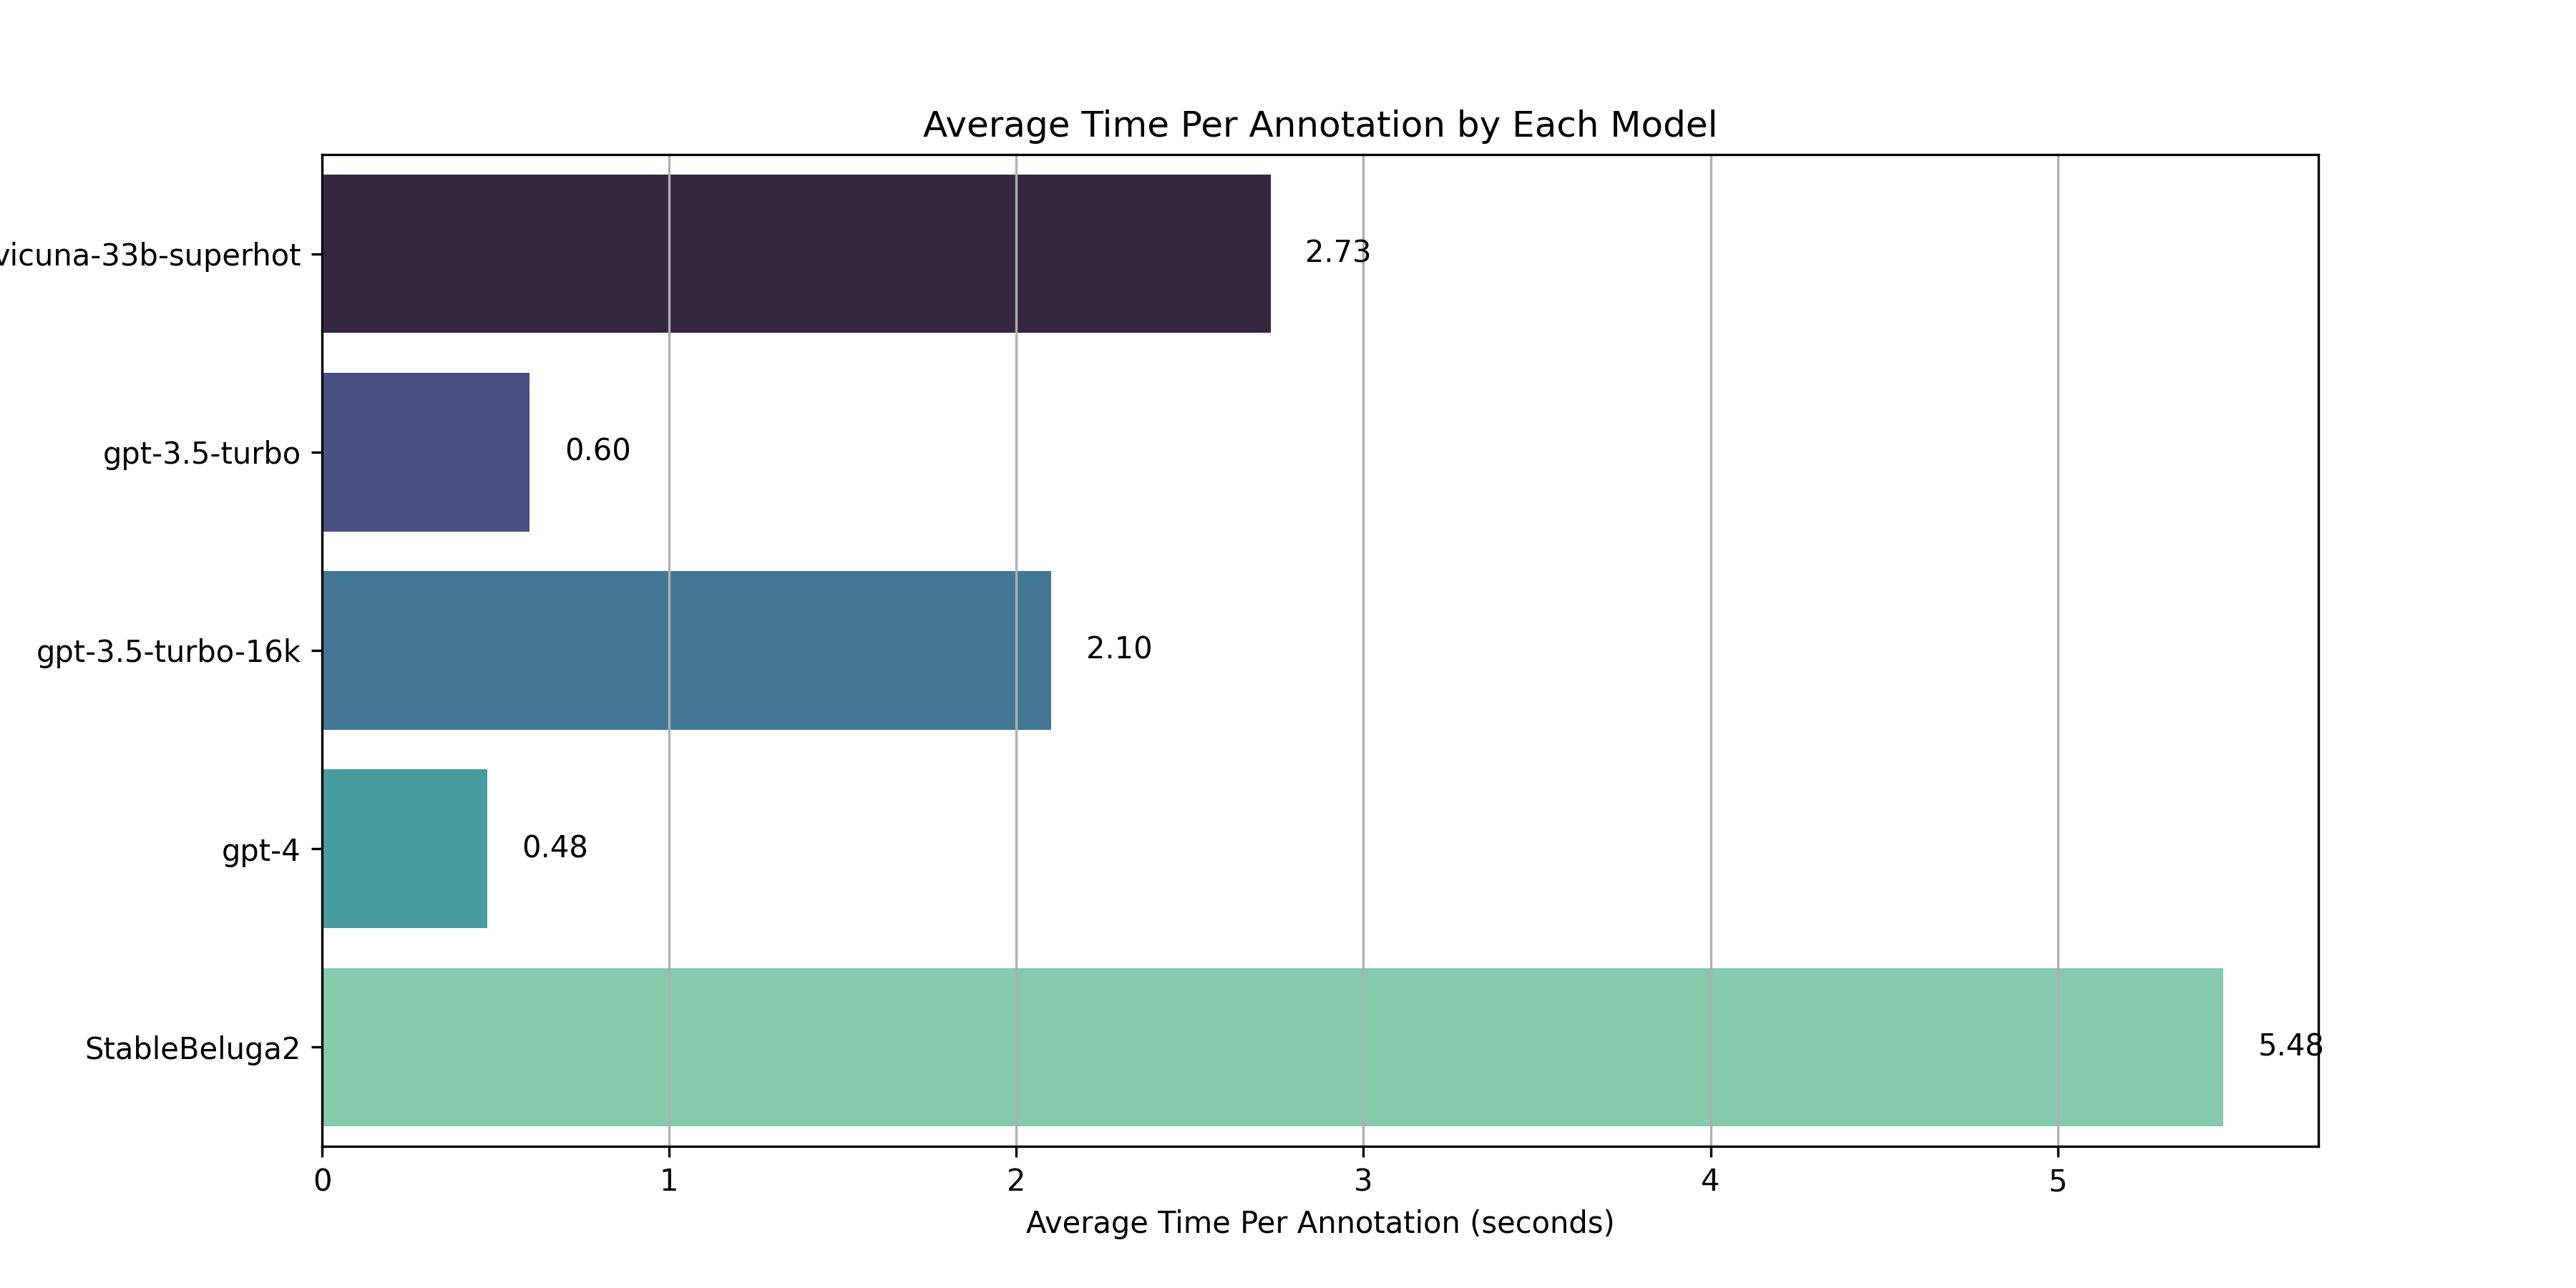
\includegraphics[width=14cm]{images/open-anno-cost.png}
  \end{tabular}
  \caption[Open Source Cost]{Average Time Taken Per Annotation by all five models}\label{fig:open-relative-cost}
\end{figure}

\begin{figure}[htpb]
  \centering
  \begin{tabular}{c}
  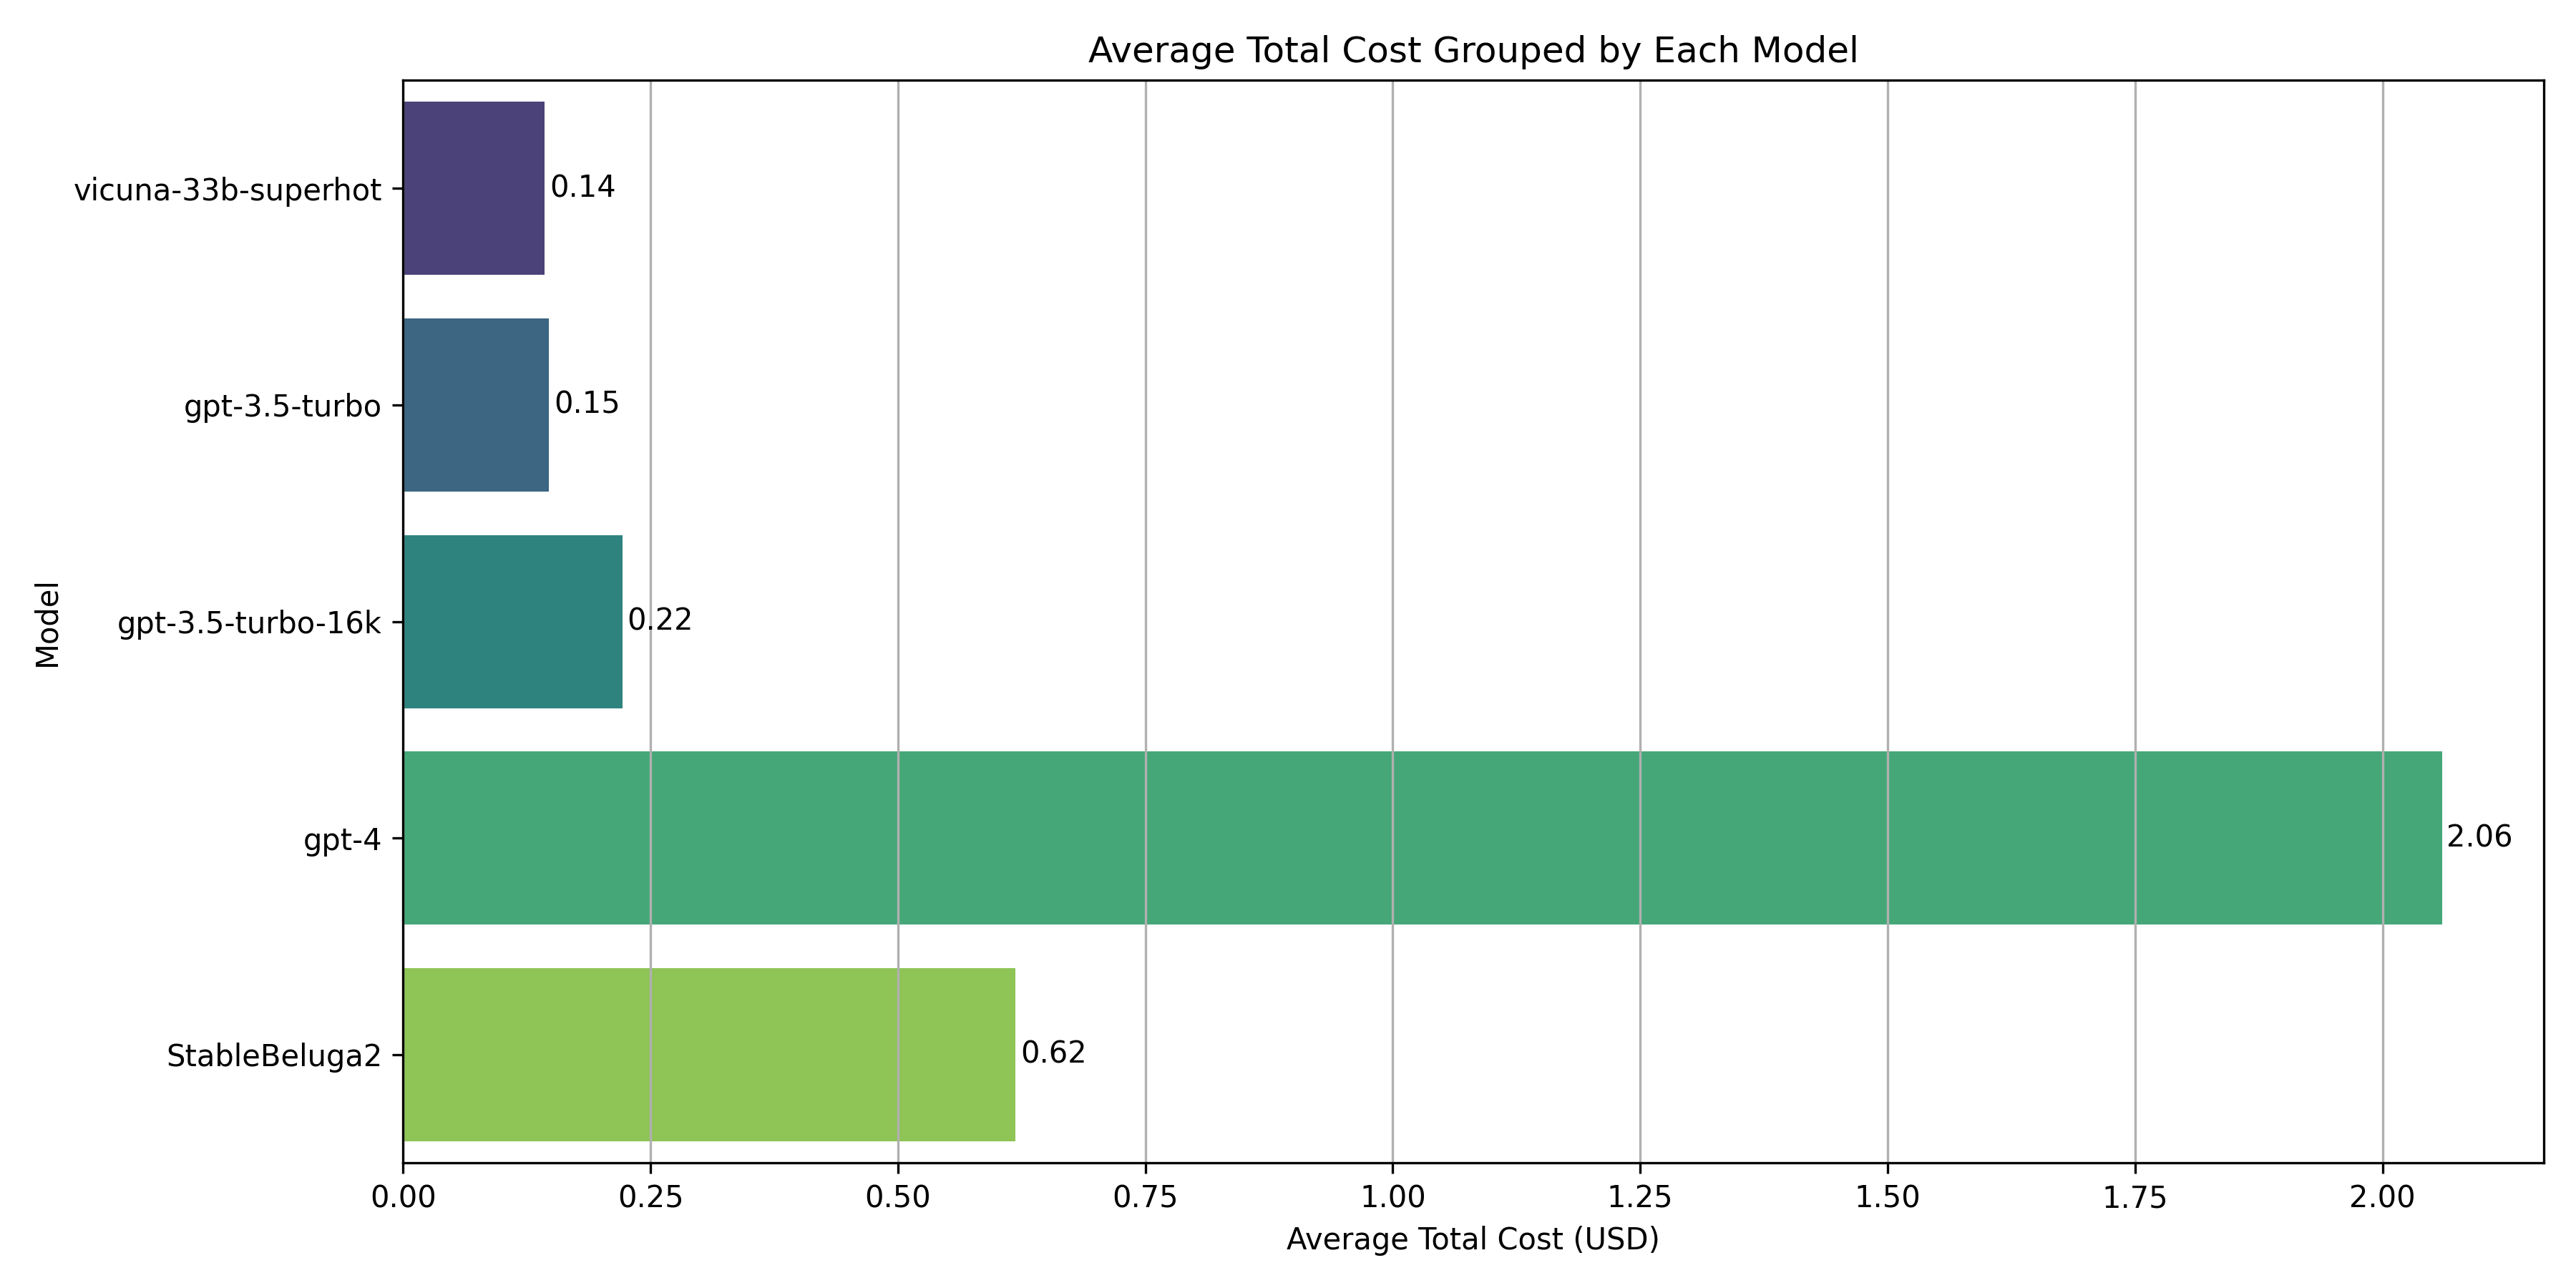
\includegraphics[width=14cm]{images/open-cost.png}
  \end{tabular}
  \caption[Open Source Time]{Average Paid Cost by all five models}\label{fig:open-cost}
\end{figure}

\section{Evaluating Potential Correlations}

Upon completion of our results assessment, it was fundamental to investigate potential correlations inherent in the received data. We probed two areas of interest: a potential correlation between the CoNLL Score and Semantic Accuracy and a possible linkage between the CoNLL Score and the paper's publication date. These examinations were crucial to determine whether any part of the original paper was contained within OpenAI's training data.

\subsection{Connection Between CoNLL Score and Semantic Accuracy}

Given that these two metrics reflect distinct facets of the paper, we anticipated that little to no correlation would be discernible. Nevertheless, several statistical measures were employed to thoroughly evaluate this potential relationship: Pearson's Correlation Coefficient, Spearman's Rank Correlation, and Kendall's Tau. As seen in Table \ref{tab:spearman}, the correlation results indicate a trivial association between these metrics, as the correlation constant is virtually zero, supported further by a notable high p-value.

\begin{table}[htpb]
    \centering
    \caption{Correlation Coefficients and P-values}\label{tab:spearman}
        \begin{tabular}{lrr}
        \hline
        Method & Correlation & P-value \\
        \hline
        Pearson's Correlation Coefficient & -0.1570 & 0.5472 \\
        Spearman's Rank Correlation & -0.0006 & 0.9981 \\
        Kendall's Tau & -0.0075 & 0.9670 \\
        \hline
    \end{tabular}
\end{table}

\subsection{Influence of Publish Date on CoNLL Score}

A query was raised regarding the possibility of papers released before September 2021—presumed to be the cut-off date for building OpenAI's GPT Models training data—yielding higher CoNLL Scores than those published afterwards. The difference in average CoNLL scores between papers released before was higher by 1.63 compared to those released after the deadline. This might be attributable to the variable nature of LLMs rather than the inclusion in the training set. For post-deadline papers, the semantic accuracy was also marginally lower—by an average of 5.87\%. However, this difference did not significantly suggest being due to training data influence.
Furthermore, the use of GPT to generate novel annotations makes it improbably likely for these exact or similar outputs to exist in the training dataset and affect the results. An observation worthy of mention is that the post-2021 papers contained significantly more concepts, which may have influenced the score. Henceforth, it is reasonable to conclude that a paper being part of the training dataset or not does substantially impact the score.

\section{Overall}

In comprehensive terms, GPT-4 established itself as the most effective and priciest model, while GPT-3.5 emerged as the cheapest and fastest. All GPT models provided commendable annotations for automation purposes, with the Open Source LLM StableBeluga2 marking a significant breakthrough with its zero-cost operation and performance that is almost at par with the GPT models. 

In comprehensive terms, GPT-4 emerged as the most impressive model due to its superior performance, albeit at a higher cost. GPT-3.5 was the most cost-effective and fastest model to operate. All GPT models provided commendable annotations for automation purposes, with the Open Source LLM StableBeluga2 marking a significant breakthrough with its zero-cost operation and performance that is almost at par with the GPT models. This is particularly noteworthy, considering StableBeluga2 is a 70 billion parameter model, and GPT-4 is rumoured to be a 1.8 trillion parameter model. The instructive nature of StableBeluga2, as opposed to the general-purpose chat model design of GPT, likely contributed to its performance in formula grounding. Figure \ref{fig:total-anal} visualises the performance-to-cost ratio for all five models, which helps to choose the models for different purposes.

\begin{figure}[htpb]
  \centering
  \subfloat[Average Cost per 1000 Concept]{
    \begin{tabular}{c}
  %\hspace*{-.25cm}
  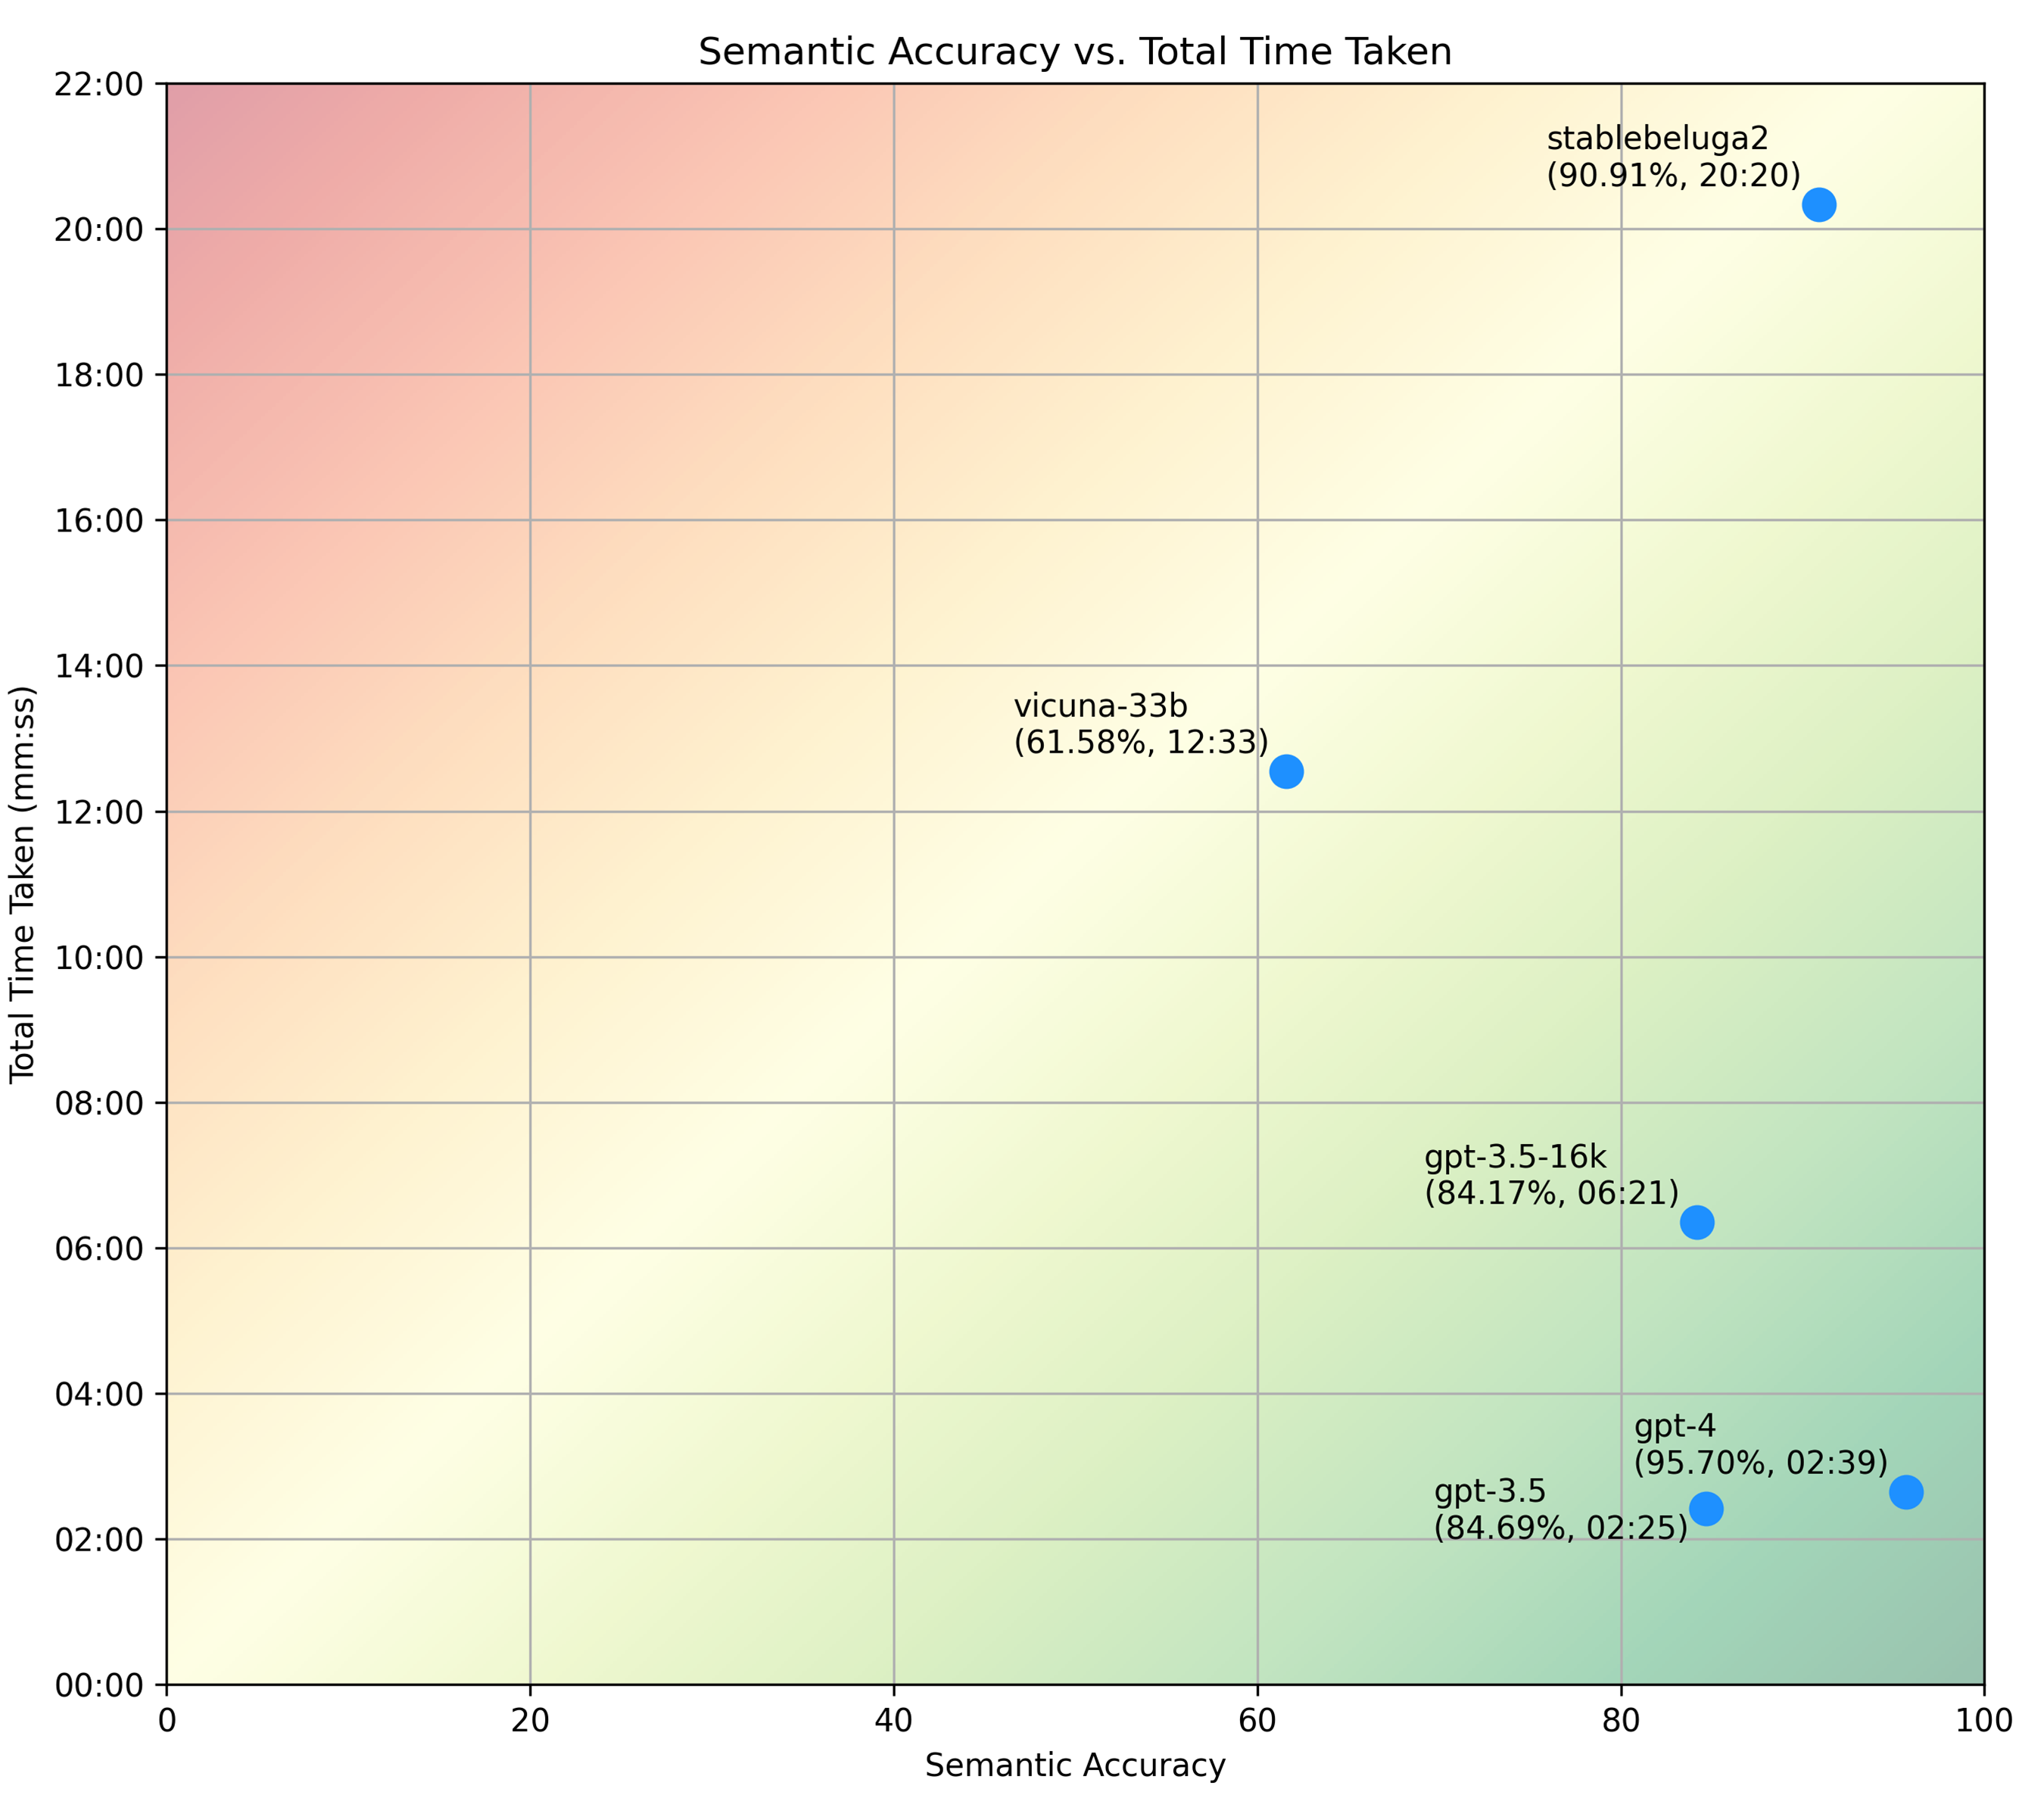
\includegraphics[width=10cm]{images/semantic-time.png}
  \end{tabular}
  }
  \quad 
  \subfloat[Average Duration per Concept]{
    \begin{tabular}{c}
  %\hspace*{-1.5cm}
  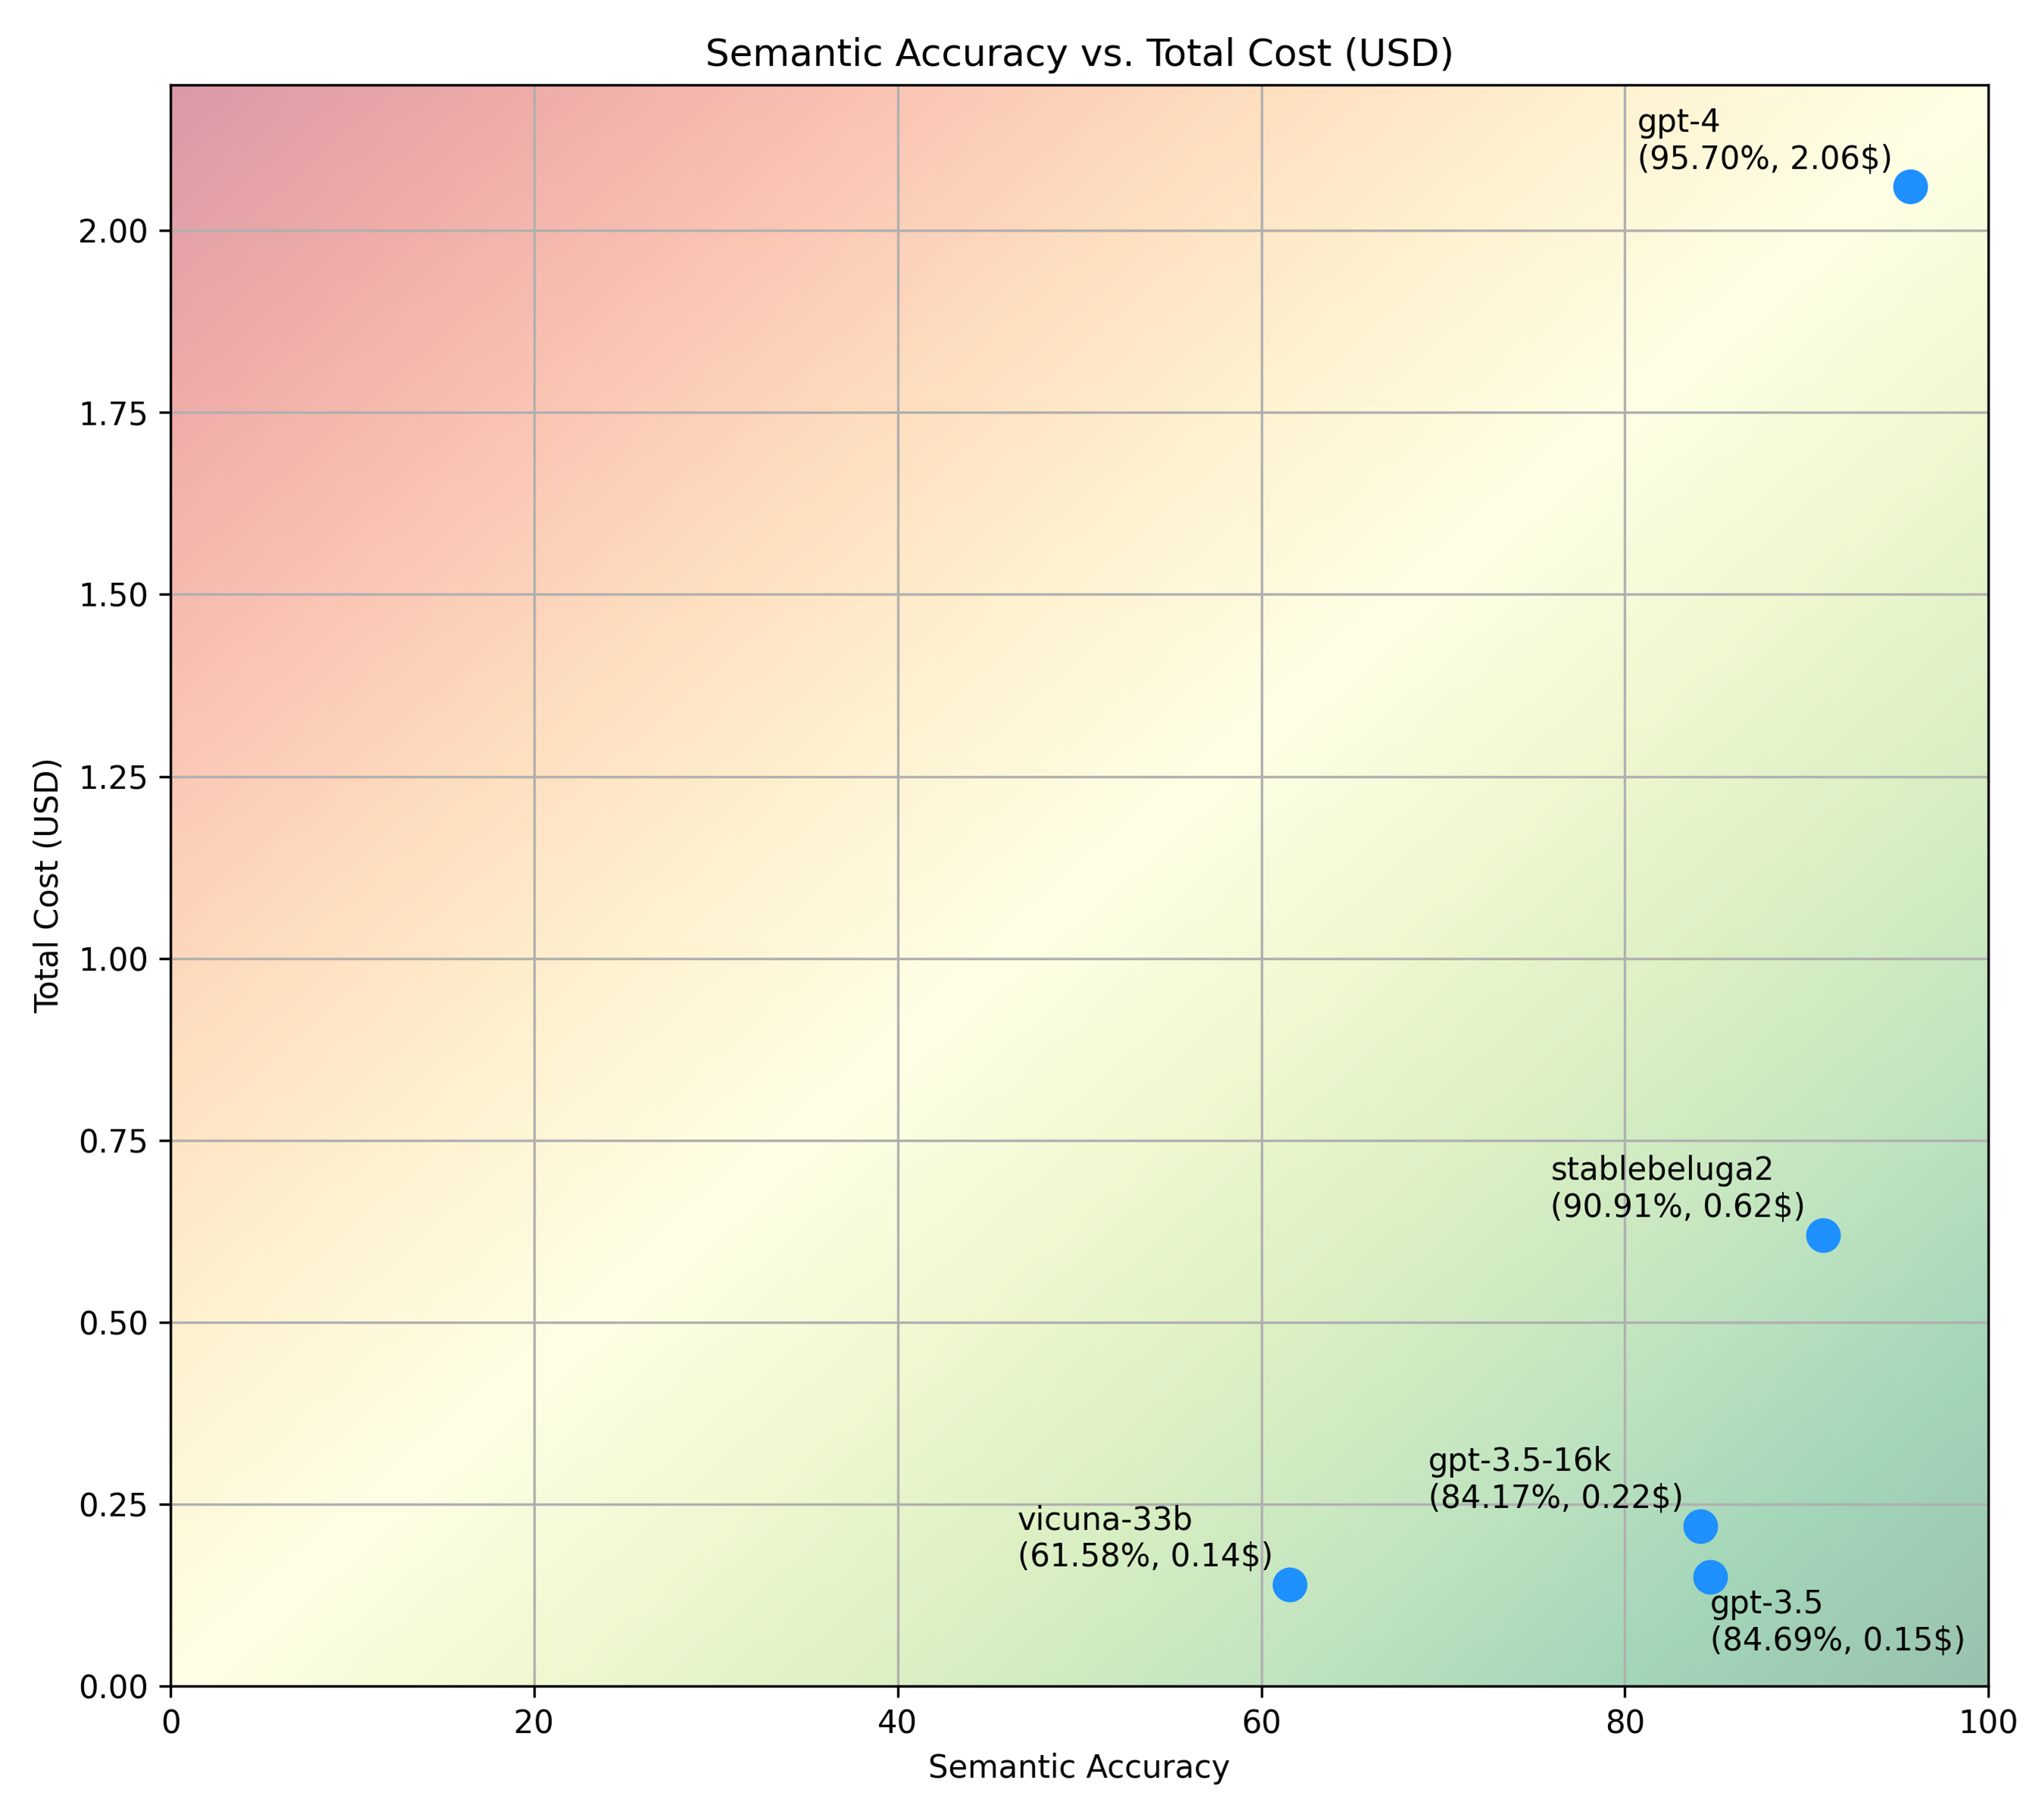
\includegraphics[width=10cm]{images/semantic-cost.png}
  \end{tabular}
  }
  \caption[Cost Analysis]{Cost and Time Usage of Automation}\label{fig:total-anal}
\end{figure}
